% !TeX spellcheck = de_CH
%%%%%%%%%%%%%%%%%%%%%%%%%%%%%%%%%%%%%%%%%%%%%%%%%%%%%%%%%%%%%%%%%
%  _____   ____  _____                                          %
% |_   _| /  __||  __ \    Institute of Computitional Physics   %
%   | |  |  /   | |__) |   Zuercher Hochschule Winterthur       %
%   | |  | (    |  ___/    (University of Applied Sciences)     %
%  _| |_ |  \__ | |        8401 Winterthur, Switzerland         %
% |_____| \____||_|                                             %
%%%%%%%%%%%%%%%%%%%%%%%%%%%%%%%%%%%%%%%%%%%%%%%%%%%%%%%%%%%%%%%%%
%
% Project     : BA Welti Keller
% Title       : 
% File        : doc.tex Rev. 00
% Date        : 15.09.2014
% Author      : Tobias Welti
%
%%%%%%%%%%%%%%%%%%%%%%%%%%%%%%%%%%%%%%%%%%%%%%%%%%%%%%%%%%%%%%%%%

%%%%%%%%%%%%%%%%%%%%%%%%%%%%%%%%%%%%%%%%%%%%%%%%%%%%%%%%%%%%%%%%%
%  _____   ____  _____                                          %
% |_   _| /  __||  __ \    Institute of Computitional Physics   %
%   | |  |  /   | |__) |   Zuercher Hochschule Winterthur       %
%   | |  | (    |  ___/    (University of Applied Sciences)     %
%  _| |_ |  \__ | |        8401 Winterthur, Switzerland         %
% |_____| \____||_|                                             %
%%%%%%%%%%%%%%%%%%%%%%%%%%%%%%%%%%%%%%%%%%%%%%%%%%%%%%%%%%%%%%%%%
%
% Project     : Konzept BA Welti Keller
% Title       : 
% File        : header.tex Rev. 00
% Date        : 15.09.2014
% Author      : Tobias Welti
%
%%%%%%%%%%%%%%%%%%%%%%%%%%%%%%%%%%%%%%%%%%%%%%%%%%%%%%%%%%%%%%%%%

\documentclass[twoside,10pt,parskip=half,ngerman]{scrreprt}

%***********************************************************************
% include some libs
%***********************************************************************	
\usepackage[utf8]{inputenc}
\usepackage{listings}
\usepackage{color}
\usepackage{fancyhdr}
\usepackage{rotating}
\usepackage{titlesec}
\usepackage{mathptmx}
\usepackage{todonotes}
 \usepackage{helvet}
%\usepackage[scaled]{uarial}
\renewcommand*\familydefault{\sfdefault} %% Only if the base font of the document is to be sans serif
\usepackage[T1]{fontenc}
\usepackage{ngerman}
\usepackage{textcomp}
\usepackage[squaren]{SIunits}
\usepackage{graphicx}
\usepackage[hyphens]{url}
\usepackage{geometry}
\usepackage[absolute]{textpos}
\usepackage{makeidx}
\usepackage{colortbl}
\usepackage{pdflscape}
\usepackage{pdfpages}
\usepackage{tabularx}
\usepackage{lmodern}
\usepackage{longtable}
\usepackage{array}
\usepackage{float}
\usepackage{scrhack}
\usepackage[plainpages=false]{hyperref}
\usepackage{wallpaper}
\usepackage{hyperref}
\urlstyle{same}

% Glossar
\usepackage[toc,nopostdot,acronyms]{glossaries}
%\usepackage{glossaries-german}
\renewcommand*{\glossaryname}{Glossar}
\renewcommand*{\acronymname}{Abkürzungsverzeichnis}
\setacronymstyle{long-short}
\makeglossaries
\loadglsentries{content/glossar}
%\makenoidxglossaries




% Deutsches Literaturverzeichnis
\usepackage{bibgerm}
% Silbentrennung (Neu-Deutsch)
 \usepackage[ngerman]{babel}
 % Spezialseiten (Literarturverzeichnis, Abbildungsverzeichnis, usw.) in Inhaltsverzeichnis anzeigen
\usepackage[nottoc]{tocbibind}

% Grafiken
%\usepackage[pdftex]{graphicx}
%\usepackage{epsfig}

%***********************************************************************
% various styles
%***********************************************************************	

%create index
\makeindex

%define pagestyle
\pagestyle{fancy}

%use sans-serif font 
%\renewcommand{\familydefault}{\sfdefault}

%define page margin
\geometry{a4paper, top=30mm, left=30mm, right=30mm, bottom=30mm,headsep=10mm,footskip=10mm}

%textpos parameter
\setlength{\TPHorizModule}{30mm}
\setlength{\TPVertModule}{\TPHorizModule}
\textblockorigin{10mm}{10mm} % start everything near the top-left corner
\setlength{\parindent}{0pt}

%horizontal lines for titlepage 
\newcommand{\HRule}{\rule{\linewidth}{0.5mm}}

%reference to source items inlc source number
\newcommand{\srcref}[1]{\nameref{src:#1} \cite{#1}}

%header / footer 
\renewcommand{\headrulewidth}{0.3pt}
\renewcommand{\footrulewidth}{0.3pt}

\fancyhead[LO,RE]{} %clear headings for contents 
\fancyhead[RO,LE]{\nouppercase{\rightmark}} %right odd pages and left even pages
\fancyhead[LO,RE]{\MakeUppercase{\leftmark}} %left odd pages and right even pages
\fancyfoot[LE,RO]{\thepage} %page numbering
\fancyfoot[C]{} %clear centered page numbering 

%define some colors
\definecolor{gray}{rgb}{0.95,0.95,0.95}
\definecolor{darkgray}{rgb}{0.4,0.4,0.4}
%listing colors
\definecolor{lgray}{RGB}{250,250,250}
\definecolor{lgreen}{RGB}{63,127,95}
\definecolor{lred}{RGB}{127,0,85}
\definecolor{lblue}{RGB}{42,0,255}

%***********************************************************************
% listing
%***********************************************************************

\lstset{		
		basicstyle=\small\ttfamily,
		frame=single,
		numbers=left,	
		numberstyle=\tiny,
		%firstnumber=auto,
		numberblanklines=true,
		captionpos=b,
		extendedchars=true,
		float=ht,
		showtabs=false,
		tabsize=2,
		showspaces=false,
		showstringspaces=false,
		breaklines=true,
		%prebreak=\Righttorque,
		backgroundcolor=\color{lgray},
		keywordstyle=\color{lred}\bfseries, 
		commentstyle=\color{lgreen}\ttfamily,
%		morekeywords={printstr, printhexln},
		stringstyle=\color{lblue},
		xleftmargin=0.5cm,
		xrightmargin=0.5cm
}

\lstloadlanguages{C++}

%\lstdefinelanguage{xc}{
%     keywords={printstr, printhexln, attributes, class, classend, do, empty, endif, endwhile, fail, function, functionend, if, implements, in, inherit, inout, not, of, operations, out, return, set, then, types, while, use},
%     keywordstyle=\color{lred}\bfseries,
%     ndkeywords={},
%     ndkeywordstyle=\color{yellow}\bfseries,
%     identifierstyle=\color{black},
%     sensitive=false,
%     comment=[l]{//},
%     commentstyle=\color{lgreen}\ttfamily,
%     string=[l]{"},
%     stringstyle=\color{lblue}\ttfamily
%  }


\begin{document}
\title{Bachelorarbeit (IT)}
\author{Tobias Keller, Tobias Welti}

% !TeX spellcheck = de_CH
%%%%%%%%%%%%%%%%%%%%%%%%%%%%%%%%%%%%%%%%%%%%%%%%%%%%%%%%%%%%%%%%%
%  _____   ____  _____                                          %
% |_   _| /  __||  __ \    Institute of Computitional Physics   %
%   | |  |  /   | |__) |   Zuercher Hochschule Winterthur       %
%   | |  | (    |  ___/    (University of Applied Sciences)     %
%  _| |_ |  \__ | |        8401 Winterthur, Switzerland         %
% |_____| \____||_|                                             %
%%%%%%%%%%%%%%%%%%%%%%%%%%%%%%%%%%%%%%%%%%%%%%%%%%%%%%%%%%%%%%%%%
%
% Project     : BA Welti Keller
% Title       : 
% File        : titlepage.tex Rev. 00
% Date        : 15.09.2014
% Author      : Tobias Welti
%
%%%%%%%%%%%%%%%%%%%%%%%%%%%%%%%%%%%%%%%%%%%%%%%%%%%%%%%%%%%%%%%%%

\begin{titlepage}

% Logo
\ThisTileWallPaper{\paperwidth}{\paperheight}{images/logos/InES.pdf} % {}images/logos/*.pdf}
% Wählen Sie aus folenden pdf Files: ICP, IDP, IEFE, IMES, IMPE, IMS, INE, InES, InIT, KSR, SoE, ZAMP, ZAV, ZIL, ZPP, ZSN

\begin{minipage}[b]{0.117\textwidth}
\hskip 0.05cm
\end{minipage}
\begin{minipage}[b]{0.91\textwidth}
\begin{tiny}.\end{tiny}\vskip 2.8cm
	{\huge
	
	% Projekt Name
	\textbf{\underline{Bachelorarbeit}}
	
	% Projekt Titel
	Messstation zur Registrierung von Geschiebe-Bewegungen im Fluss
	\vskip 0.5cm}
	
	\begin{minipage}[b]{0.27\textwidth}
	\hrule\vskip 0.5cm
		\textbf{Autoren}\\
		\\
	\end{minipage}
	\begin{minipage}[b]{0.03\textwidth}
	\hskip 0.5cm
	\end{minipage}
	\begin{minipage}[b]{0.7\textwidth}
	\hrule\vskip 0.5cm
		Tobias Keller\\
		Tobias Welti\\
	\end{minipage}
	
	\begin{minipage}[b]{0.27\textwidth}
	\hrule\vskip 0.5cm
		\textbf{Betreuer}\\
		\\
	\end{minipage}
	\begin{minipage}[b]{0.03\textwidth}
	\hskip 0.5cm
	\end{minipage}
	\begin{minipage}[b]{0.7\textwidth}
	\hrule\vskip 0.5cm
		Prof. Hans-Joachim Gelke, Dipl. El. Ing. FH\\
		ZHAW Institute for Embedded Systems\\
	\end{minipage}
	
	\begin{minipage}[b]{0.27\textwidth}
	\hrule\vskip 0.5cm
		\textbf{Partner}\\
		\\
	\end{minipage}
	\begin{minipage}[b]{0.03\textwidth}
	\hskip 0.5cm
	\end{minipage}
	\begin{minipage}[b]{0.7\textwidth}
	\hrule\vskip 0.5cm
	  Carlos Rodrigo Wyss\\
		Eidg. Forschungsanstalt für Wald, Schnee und Landschaft WSL\\
	\end{minipage}
	
	\begin{minipage}[b]{0.27\textwidth}
	\hrule\vskip 0.5cm
		\textbf{Datum}
	\end{minipage}
	\begin{minipage}[b]{0.03\textwidth}
	\hskip 0.5cm
	\end{minipage}
	\begin{minipage}[b]{0.7\textwidth}
	\hrule\vskip 0.5cm
		\today
	\end{minipage}
\end{minipage}
\vskip 0.5cm

\end{titlepage}


\includepdf{images/Erklaerung_BA.pdf}
%%%%%%%%%%%%%%%%%%%%%%%%%%%%%%%%%%%%%%%%%%%%%%%%%%%%%%%%%%%%%%%%%
%  _____   ____  _____                                          %
% |_   _| /  __||  __ \    Institute of Computitional Physics   %
%   | |  |  /   | |__) |   Zuercher Hochschule Winterthur       %
%   | |  | (    |  ___/    (University of Applied Sciences)     %
%  _| |_ |  \__ | |        8401 Winterthur, Switzerland         %
% |_____| \____||_|                                             %
%%%%%%%%%%%%%%%%%%%%%%%%%%%%%%%%%%%%%%%%%%%%%%%%%%%%%%%%%%%%%%%%%
%
% Project     : BA Welti Keller
% Title       : 
% File        : abstract.tex Rev. 00
% Date        : 15.09.2014
% Author      : Tobias Welti
%
%%%%%%%%%%%%%%%%%%%%%%%%%%%%%%%%%%%%%%%%%%%%%%%%%%%%%%%%%%%%%%%%%

\thispagestyle{empty}
\chapter*{Zusammenfassung}\label{chap.zusammenfassung}
Zurzeit kommen zur Messung von Geschiebebewegungen in Gewässern diverse Lösungen zur Anwendung. Bei der Eidg. Forschungsanstalt für Wald, Schnee und Landschaft (WSL) werden hauptsächlich Geophone verwendet, welche kostspielig sind und aufwändige bauliche Massnahmen sowie eine verhältnismässig komplexe IT-Infrastruktur bedingen. Das Erstellen eines Prototypen, der die Vereinfachung dieses Systems durch die Konzeption eines geeigneten Bussystems und der Verwendung kompakter MEMS-Beschleunigungssensoren zur Ereigniserkennung demonstriert, war das Hauptziel dieser Arbeit.

Als Basis für die im Einsatz befindlichen Geräte dienen Boards mit einem ARM Cortex-M4 Mikrocontroller. Das konzipierte System besteht im wesentlichen aus zwei Komponenten: einem Datenlogger und den Sensoreinheiten. Der Datenlogger zeichnet die Messwerte auf einer SD-Karte auf und übernimmt die Konfiguration der angehängten Sensoreinheiten. Im Unterschied zum normalen CAN-Bus muss der Absender einer Meldung für das Bus-Protokoll identifizierbar sein. Deshalb fungiert der Datenlogger auch als Busmaster und weist den Teilnehmern am CAN-Bus eindeutige Identifikationen zu. Die Sensoreinheiten bestehen aus den MEMS-Beschleunigungssensoren und dem Mikrocontroller, der die Messdaten je nach gewähltem Modus verarbeitet. Möglich ist dabei das Aufzeichnen der wichtigsten Kenndaten eines Ereignisses, die detailreiche Aufzeichnung eines Einschlages in zwei Detailstufen oder das Senden der Rohdaten eines Sensors. Durch die direkt im Sensor stattfindende Verarbeitung der Messdaten wird einerseits der Bus entlastet. Es werden nur die verarbeiteten Daten übermittelt. Andererseits fällt für den Datenlogger weniger Arbeit an, da dieser keine Sensordaten auswerten muss und nur noch die fertigen Daten speichert.

Da das ganze System unter anderem in Gebirgsbächen eingesetzt werden soll, musste ein besonderes Augenmerk auf die Stabilität und die Autarkie der Lösung gelegt werden. Wurde die Konfiguration des System einmal manuell vorgenommen, so können die Werte abgespeichert und bei einem Neustart des Systems automatisch wieder geladen werden. Die Verwendung eines CAN-Busses garantiert zudem die fehlerfreie Übertragung der Daten. 

Der erstellte Prototyp erfüllt die Erwartungen in Bezug auf die Vereinfachung des Aufbaus und den Verbrauch des ganzen Systems. Er könnte somit als Basis für ein finales Produkt dienen.



\newpage
\thispagestyle{empty}
\chapter*{Abstract}\label{abstract}
There are different ways to measure the transportation of bed load. The most common one, also used by the Swiss Federal Institute for Forest, Snow and Landscape Research (WSL), being the mounting of geophones in the river bed. There are several disadvantages to this, the main ones being the costs involved and the necessary structural measures. 

Additionally, the IT infrastructure becomes rather complex, since the geophones are connected by one cable each to an industrial, rugged PC. The goal of this project is to plan, design and implement a bus-system with MEMS-accelerometers and provide a prototype of a simpler and more cost-efficient measurement installation than the usage of geophones.

All used devices are based on the ARM Cortex-M4 microcontroller. The system implemented consists of two types of devices, the data logger and the sensor units. The data logger  receives and stores the processed data transmitted by the sensors. Additionally, the logger acts as a bus master and configures all the connected devices by sending them unique identifiers, thusly allowing for a proper assignment of the received messages to each sensor. The sensor units are composed of a MEMS-accelerometer and a microcontroller that processes the measurements from the MEMS, packaging the data depending on the detail level specified by the user, effectively reducing the traffic on the bus and the workload for the data logger. The detail level can be set dynamically by the user to either log the basic data of an impact, the detailed data of an impact (two levels of details are possible) or to send unprocessed raw data over a time range.

Since the whole system will be installed in rivers it should be rugged and self-sustaining. Once configured, the settings for each sensor can be stored on the SD card of the logger and, if a reset should occur, will be read automatically and sent to the sensors. The usage of a CAN-bus guarantees the error free transmission of the measured data.

The built prototype fulfills the expectations concerning the simplification of the system and the resource usage of the system and therefore could be used as a base for a final product.




% !TeX spellcheck = de_CH
%%%%%%%%%%%%%%%%%%%%%%%%%%%%%%%%%%%%%%%%%%%%%%%%%%%%%%%%%%%%%%%%%
%  _____   ____  _____                                          %
% |_   _| /  __||  __ \    Institute of Computitional Physics   %
%   | |  |  /   | |__) |   Zuercher Hochschule Winterthur       %
%   | |  | (    |  ___/    (University of Applied Sciences)     %
%  _| |_ |  \__ | |        8401 Winterthur, Switzerland         %
% |_____| \____||_|                                             %
%%%%%%%%%%%%%%%%%%%%%%%%%%%%%%%%%%%%%%%%%%%%%%%%%%%%%%%%%%%%%%%%%
%
% Project     : BA Welti Keller
% Title       : 
% File        : vorwort.tex Rev. 00
% Date        : 15.09.2014
% Author      : Tobias Welti
%
%%%%%%%%%%%%%%%%%%%%%%%%%%%%%%%%%%%%%%%%%%%%%%%%%%%%%%%%%%%%%%%%%

\chapter*{Vorwort}\label{chap.vorwort}
Durch eine Studienkollegin kamen wir im Sommer 2013 mit Bruno Fritschi von der Eidgenössischen Forschungsanstalt für Wald, Schnee und Landschaft (WSL) in Kontakt und konnten uns von ihm einige äusserst interessante Ideen für Bachelorarbeiten im Bereich Embedded Systems vorstellen lassen. Ziemlich schnell waren wir uns einig, dass die Entwicklung eines Bussystems zur Messung von Geschiebetransport nach einer spannenden und herausfordernden Aufgabe tönt und entschlossen uns, diese als Bachelorarbeit anzugehen. Wie wir feststellen mussten, ist die Planung und Implementation eines ganzen Systems eine ziemliche Herausforderung, zumal wir beide bis jetzt nur wenig Erfahrung in diesem Bereich gesammelt hatten. Dank dem fachlichen Know-how von Bruno Fritschi und Hans Gelke konnten wir zum Schluss einen funktionierenden Prototyp erstellen, der zumindest die Machbarkeit dieser Lösung bestätigt. Es gibt aber durchaus noch einige Punkte, die man verbessern oder erweitern muss, bevor man von einem finalen Produkt sprechen kann.

\setcounter{page}{1}
\include{content/kontakt}


%Inhaltsverzeichnis
\tableofcontents
\listoftodos
\newpage


%Kapitel
%\setcounter{page}{1}
%\pagenumbering{arabic}

% !TeX spellcheck = de_CH
%%%%%%%%%%%%%%%%%%%%%%%%%%%%%%%%%%%%%%%%%%%%%%%%%%%%%%%%%%%%%%%%%
%  _____   ____  _____                                          %
% |_   _| /  __||  __ \    Institute of Computitional Physics   %
%   | |  |  /   | |__) |   Zuercher Hochschule Winterthur       %
%   | |  | (    |  ___/    (University of Applied Sciences)     %
%  _| |_ |  \__ | |        8401 Winterthur, Switzerland         %
% |_____| \____||_|                                             %
%%%%%%%%%%%%%%%%%%%%%%%%%%%%%%%%%%%%%%%%%%%%%%%%%%%%%%%%%%%%%%%%%
%

% Project     : Pflichtenheft BA Welti Keller
% Title       : 
% File        : einleitung.tex Rev. 00
% Date        : 15.09.2014
% Author      : Tobias Welti
%
%%%%%%%%%%%%%%%%%%%%%%%%%%%%%%%%%%%%%%%%%%%%%%%%%%%%%%%%%%%%%%%%%

\chapter{Einleitung}\label{chap.einleitung}



\section{Ausgangslage}\label{sec.ausgangslage}
Die Eidg. Forschungsanstalt für Wald, Schnee und Landschaft (WSL) betreibt Messstationen zur Registrierung von Geschiebe-Bewegungen im Fluss mittels Geophonen, die unter Stahlplatten montiert sind. Diese Platten sind in einer Betonkonstruktion eingelassen, um sie im Flussbett zu fixieren. Die Geophone sind über Kabel mit einem Auswertungs-Rechner (Embedded PC) verbunden, der die Signale auswertet. Die baulichen Massnahmen für die Installation der Sensoren, der Auswertungsstation sowie der Stromversorgung sind sehr teuer. 


\section{Aufgabenstellung}\label{sec.aufgabenstellung}
Im Rahmen dieser Bachelorarbeit soll eine Lösung erarbeitet werden, um zukünftige Installationen günstiger zu machen. Da solche Messanlagen an sehr vielen Orten auf der ganzen Welt aufgebaut werden, kann durch eine Vereinfachung der Installation viel Aufwand gespart werden. 

Die Projektidee stammt von Bruno Fritschi (WSL). Sein Vorschlag sieht vor, die aufgezeichneten Signale direkt am Sensor auszuwerten und nur die gewünschten Ereignisse zu übertragen und zu speichern. Somit könnten die Daten über ein Bussystem übertragen werden und der Auswertungsrechner bräuchte weniger Leistung.

Dank der Bustopologie ist das Messsystem weniger komplex und kann einfacher installiert werden. Denkbar wäre die Integration in einer Gummimatte anstelle der Stahl- und Betonkonstruktion, da viel weniger Leitungen nötig sind.

Ziel der Arbeit ist die Entwicklung der Auswertungshardware und des Bussystems. Die Qualität der gemessenen Signale soll mindestens erhalten werden. Die Auswertungsalgorithmen sind nicht Bestandteil der Arbeit und werden vom WSL zur Verfügung gestellt.

Die von der bisherigen Anlage gemachten Messdaten enthalten die Dauer und Intensität jedes Aufschlags (Ereignis) auf der Sensorplatte, sowie die Anzahl Ausschläge (Peaks) pro Aufschlag. Pro Minute wird ein Histogramm über die Intesitäten der Peaks gebildet und abgespeichert.

Denkbar wäre es, einen Prototyp für Vergleichsmessungen im Erlenbach (Alptal, SZ) an einer bestehenden Schwelle zu implementieren.

\subsection{Musskriterien}
\begin{itemize}
\item Die Anlage zeichnet den Geschiebetransport im Bachbett auf. Die bisherige Aufzeichnungsrate von 10'000 Messpunkten pro Sekunde soll nicht unterschritten werden.
\item Die Anlage liefert eine minütliche Zusammenfassung über die Ereignisse an jedem Sensor. Diese Zusammenfassung enthält die Anzahl, Dauer und Intensität der einzelnen Ereignisse sowie ein Histogramm über die Intensitätsverteilung.
\item Die Messstation ist fähig, mindestens zehn Sensoren zu betreiben und ihre Messignale aufzuzeichnen.
\item Es ist möglich, die kompletten Rohdaten von einem Sensor über eine Dauer von 30 Minuten aufzuzeichnen. Während einer solchen Messung dürfen die anderen Sensoren ihre Messung einstellen.
\item Die Sensoren können über bis zu fünfzehn Meter im Bachbett verteilt sein.
\item Die Leistungsaufnahme der Anlage beim Betrieb von 10 Sensoren ist kleiner als zehn Watt.
\item Die Datenaufzeichnung erfolgt in einem eigens entwickelten Datenlogger.
\item Am Datenlogger kann ein Laptop angeschlossen werden, um Kontrollparameter der Messanlage zu setzen und um den Status der Anlage abzufragen.
\item Die erfassten Messdaten werden im Datenlogger auf einer Speicherkarte gespeichert. Dies ermöglicht ein einfaches Abholen der Daten im Feld, indem die Speicherkarte ausgetauscht wird.
\end{itemize}
\subsection{Wunschkriterien}
\begin{itemize}
\item Die Anlage liefert für jedes Ereignis die Rohdaten in voller zeitlicher Auflösung.
\item Der Sensoraufbau ermöglicht es, die Sensoren in einer Elastomerplatte zu verpacken. Die Elastomerplatte kann ohne Betonkonstruktion im Bachbett verankert werden.
\item Am Datenlogger kann ein Laptop angeschlossen werden, um die erfassten Messdaten herunterzuladen.
\end{itemize}
\subsection{Abgrenzungskriterien}
\begin{itemize}
\item Es würde den Rahmen dieser Arbeit sprengen, die Messeinheiten zur Produktreife zu bringen. Es wird lediglich aufgezeigt, wie solche Messeinheiten realisiert werden könnten.
\item Eine Testinstallation in einem Bach ist nicht möglich. Allenfalls kann in der Versuchsanstalt für Wasserbau, Hydrologie und Glaziologie der ETH Zürich ein kleiner Testlauf stattfinden.
\item
\end{itemize}

% !TeX spellcheck = de_CH
%%%%%%%%%%%%%%%%%%%%%%%%%%%%%%%%%%%%%%%%%%%%%%%%%%%%%%%%%%%%%%%%%
%  _____   ____  _____                                          %
% |_   _| /  __||  __ \    Institute of Computitional Physics   %
%   | |  |  /   | |__) |   Zuercher Hochschule Winterthur       %
%   | |  | (    |  ___/    (University of Applied Sciences)     %
%  _| |_ |  \__ | |        8401 Winterthur, Switzerland         %
% |_____| \____||_|                                             %
%%%%%%%%%%%%%%%%%%%%%%%%%%%%%%%%%%%%%%%%%%%%%%%%%%%%%%%%%%%%%%%%%
%
% Project     : BA Welti Keller
% Title       : 
% File        : aufgabenstellung.tex Rev. 00
% Date        : 15.09.2014
% Author      : Tobias Welti
%
%%%%%%%%%%%%%%%%%%%%%%%%%%%%%%%%%%%%%%%%%%%%%%%%%%%%%%%%%%%%%%%%%

\chapter{Aufgabenstellung}\label{chap.aufgabenstellung}

Die offizielle Aufgabenstellung befindet sich im Anhang \ref{app.aufgabenstellung}.

\section{Aufgabenstellung}\label{sec.aufgabenstellung}
Im Rahmen dieser Bachelorarbeit soll eine Lösung erarbeitet werden, um zukünftige Installationen günstiger zu machen. Da solche Messanlagen an sehr vielen Orten auf der ganzen Welt aufgebaut werden, kann durch eine Vereinfachung der Installation viel Aufwand gespart werden. 

Die Projektidee stammt von Bruno Fritschi (WSL). Sein Vorschlag sieht vor, die aufgezeichneten Signale direkt am \gls{sensor} auszuwerten und nur die gewünschten \gls{ereignis}-Daten zu übertragen und zu speichern. Somit könnten die Daten über ein \gls{bussys} übertragen werden und der Rechner für die Sammlung der Daten bräuchte weniger Rechenleistung.

Dank der Bustopologie kommt das Messsystem mit weniger Leitungen aus und kann einfacher installiert werden. Denkbar wäre die Integration in einer Elastomerplatte anstelle der Stahl- und Betonkonstruktion, da viel weniger Leitungen nötig sind. Die Elastomerplatte könnte einfacher im Bachbett verankert werden.

Ziel der Arbeit ist die Entwicklung der Auswertungshardware und des \gls{bussys}s. Die Qualität der gemessenen Signale soll mindestens erhalten werden. Die Auswertungsalgorithmen sind nicht Bestandteil der Arbeit und werden vom WSL zur Verfügung gestellt.

Die von der bisherigen Anlage gemachten Messdaten enthalten die Dauer und Intensität jedes Aufschlags (\gls{ereignis}) auf der Sensorplatte, sowie die Anzahl Ausschläge (Peaks) pro Aufschlag. Pro Minute wird ein Histogramm über die Intesitäten der Peaks gebildet und abgespeichert.

Denkbar wäre es, einen Prototyp für Vergleichsmessungen im Erlenbach (Alptal, SZ) an einer bestehenden Schwelle zu implementieren.


\subsection{Musskriterien}
\begin{itemize}
\item Die Anlage zeichnet den Geschiebetransport im Bachbett auf. Die bisherige Aufzeichnungsrate von 10'000 Messpunkten pro Sekunde soll nicht unterschritten werden.
\item Die Anlage liefert eine minütliche Zusammenfassung über die \glspl{ereignis} an jedem \gls{sensor}. Diese Zusammenfassung enthält die Anzahl, Dauer und Intensität der einzelnen \glspl{ereignis} sowie ein Histogramm über die Intensitätsverteilung.
\item Die Messstation ist fähig, mindestens zehn \glspl{sensor} zu betreiben und ihre Messignale aufzuzeichnen.
\item Es ist möglich, die kompletten Rohdaten von einem \gls{sensor} über eine Dauer von 30 Minuten aufzuzeichnen. Während einer solchen Messung dürfen die anderen \glspl{sensor} ihre Messung einstellen.
\item Die \glspl{sensor} können über bis zu fünfzehn Meter im Bachbett verteilt sein.
\item Die Leistungsaufnahme der Anlage beim Betrieb von 10 \glspl{sensor} ist kleiner als zehn Watt.
\item Die Datenaufzeichnung erfolgt in einem eigens entwickelten \gls{logger}.
\item Am \gls{logger} kann ein Laptop angeschlossen werden, um Kontrollparameter der Messanlage zu setzen und um den Status der Anlage abzufragen.
\item Die erfassten Messdaten werden im \gls{logger} auf einer Speicherkarte gespeichert. Dies ermöglicht ein einfaches Abholen der Daten im Feld, indem die Speicherkarte ausgetauscht wird.
\end{itemize}
\subsection{Wunschkriterien}
\begin{itemize}
\item Die Anlage liefert für jedes \gls{ereignis} die Rohdaten in voller zeitlicher Auflösung.
\item Der Sensoraufbau ermöglicht es, die \glspl{sensor} in einer Elastomerplatte zu verpacken. Die Elastomerplatte kann ohne Betonkonstruktion im Bachbett verankert werden.
\item Am \gls{logger} kann ein Laptop angeschlossen werden, um die erfassten Messdaten herunterzuladen.
\end{itemize}
\subsection{Abgrenzungskriterien}
\begin{itemize}
\item Es würde den Rahmen dieser Arbeit sprengen, die Messeinheiten zur Produktreife zu bringen. Es wird lediglich aufgezeigt, wie solche Messeinheiten realisiert werden könnten.
\item Eine Testinstallation in einem Bach ist nicht möglich. Allenfalls kann in der Versuchsanstalt für Wasserbau, Hydrologie und Glaziologie der ETH Zürich ein kleiner Testlauf stattfinden.
\item
\end{itemize}


% !TeX spellcheck = de_CH
%%%%%%%%%%%%%%%%%%%%%%%%%%%%%%%%%%%%%%%%%%%%%%%%%%%%%%%%%%%%%%%%%
%  _____   ____  _____                                          %
% |_   _| /  __||  __ \    Institute of Computitional Physics   %
%   | |  |  /   | |__) |   Zuercher Hochschule Winterthur       %
%   | |  | (    |  ___/    (University of Applied Sciences)     %
%  _| |_ |  \__ | |        8401 Winterthur, Switzerland         %
% |_____| \____||_|                                             %
%%%%%%%%%%%%%%%%%%%%%%%%%%%%%%%%%%%%%%%%%%%%%%%%%%%%%%%%%%%%%%%%%
%
% Project     : BA Welti Keller
% Title       : 
% File        : vorgehen.tex Rev. 00
% Date        : 15.09.2014
% Author      : Tobias Welti
%
%%%%%%%%%%%%%%%%%%%%%%%%%%%%%%%%%%%%%%%%%%%%%%%%%%%%%%%%%%%%%%%%%

\chapter{Vorgehen}\label{chap.vorgehen}

% !TeX spellcheck = de_CH
% !TeX spellcheck = de_CH
%%%%%%%%%%%%%%%%%%%%%%%%%%%%%%%%%%%%%%%%%%%%%%%%%%%%%%%%%%%%%%%%%
%  _____   ____  _____                                          %
% |_   _| /  __||  __ \    Institute of Computational Physics   %
%   | |  |  /   | |__) |   Zuercher Hochschule Winterthur       %
%   | |  | (    |  ___/    (University of Applied Sciences)     %
%  _| |_ |  \__ | |        8401 Winterthur, Switzerland         %
% |_____| \____||_|                                             %
%%%%%%%%%%%%%%%%%%%%%%%%%%%%%%%%%%%%%%%%%%%%%%%%%%%%%%%%%%%%%%%%%
%
% Project     : BA Welti Keller
% Title       : 
% File        : funktionale.tex Rev. 00
% Date        : 15.09.2014
% Author      : Tobias Welti
%
%%%%%%%%%%%%%%%%%%%%%%%%%%%%%%%%%%%%%%%%%%%%%%%%%%%%%%%%%%%%%%%%%

\thispagestyle{empty}
\chapter{Funktionale Anforderungen}\label{chap.funktionale}
\section{\gls{logger} (F1\ldots)}


\subsection{F110 Busmaster}
Der \gls{logger} übernimmt die Kontrolle des \gls{bussys}. Bei Inbetriebnahme des Systems tastet der \gls{logger} den Bus nach \glspl{sensoreinh} ab und erteilt jeder \gls{sensoreinh} eine eindeutige Identifikationsnummer (ID). Die ID des \gls{logger}s soll so gewählt werden, dass er jederzeit Priorität hat, auf den Bus zu schreiben.


\subsection{F120 Sensorerkennung}
Die angeschlossenen \glspl{sensor} werden vom \gls{logger} erkannt und mit einer ID versehen. Anhand der ID wird die Priorität bei der Datenübertragung festgelegt und der \gls{sensor} identifiziert. Ein Sensor, der bereits am System angeschlossen war, erhält wieder die gleiche \gls{id}, sofern die Konfigurationsdatei nicht gelöscht wurde.


\subsection{F130 Uhrzeit}
Der \gls{logger} verfügt über eine interne Uhr, um die \glspl{ereignis} in den Dateien mit einem lesbaren Zeitstempel zu versehen.


\subsection{F140 \gls{timestamp} verteilen}
Der \gls{logger} sendet ein Signal an alle \glspl{sensoreinh}, dass der Zeitstempel (\gls{timestamp}) neu gestellt werden soll. Ab dann beziehen sich die \gls{timestamp}s auf die Dauer seit dem jetzigen Zeitpunkt.


\subsection{F160 Schnittstelle zum Steuerrechner}
Der \gls{logger} bietet eine Schnittstelle, an der ein Steuerrechner (Laptop, \gls{pc}) angeschlossen werden kann. Über diese Schnittstelle kann der Betrieb der ganzen Anlage gesteuert werden.


\subsection{F170 Steuerung Betriebsmodus}
Der Betriebsmodus der \glspl{sensor} wird vom \gls{logger} aus gesteuert: Wie viele und welche Art von Daten gesammelt werden soll und ob alle \glspl{sensor} oder nur bestimmte aktiv sein sollen. \\
Folgende Betreibsmodi sind verfügbar:
\begin{itemize}
\item Normaler Modus: Alle \glspl{sensor} übermitteln die verarbeiteten Ereignisdaten. Zeitpunkt, Intensität, Dauer und Anzahl Ausschläge jedes \gls{ereignis} werden gespeichert.
\item Detaillierter Modus: Alle \glspl{sensor} übermitteln die verarbeiteten Ereignisdaten sowie die gesamten Messdaten für die Dauer des \gls{ereignis}.
\item Rohdatenmodus: Ein \gls{sensor} übermittelt kontinuierlich Rohdaten, die anderen \glspl{sensor} werden vorübergehend abgeschaltet.
\end{itemize}


\subsection{F180 Daten sammeln}
Der \gls{logger} fragt in regelmässigen Abständen bei den \glspl{sensoreinh} an, ob Ereignisdaten zur Übertragung bereit sind. Diese übermitteln die vorliegenden Ereignisdaten.


\subsection{F190 Daten speichern}
Die Daten werden vom \gls{logger} auf einer Speicherkarte in Dateien abgelegt. Nach entsprechenden Befehlen vom Steuerrechner kann die Karte entfernt und ausgetauscht werden, um die Daten abzuholen.


\section{\gls{sensoreinh} (F4\ldots)}


\subsection{F410 Ereignisdetektion}
Die \gls{sensoreinh} liest den \gls{sensor} mit einer definierten \gls{fs} aus und wertet die Messdaten aus. Der Prozessor erkennt \glspl{ereignis} anhand definierter Kriterien. Zu jedem \gls{ereignis} werden folgende Daten gespeichert: Zeitpunkt (\gls{timestamp}), Dauer, Anzahl Peaks und höchster Peak. In einem zweiten Betriebsmodus können alle Messpunkte während einem \gls{ereignis} gespeichert werden.


\subsection{F430 Datenübertragung}
Die \gls{sensoreinh} übermittelt die Ereignisdaten über das \gls{bussys} an den \gls{logger}.


\subsection{F450 Rohdatenaufzeichnung}
In einem Sondermodus werden alle Messpunkte gespeichert und über das \gls{bussys} an den \gls{logger} übertragen. In diesem Betriebsmodus kann darf auch nur eine \gls{sensoreinh} aktiv sein, die anderen werden auf Standby geschaltet.



% !TeX spellcheck = de_CH
%%%%%%%%%%%%%%%%%%%%%%%%%%%%%%%%%%%%%%%%%%%%%%%%%%%%%%%%%%%%%%%%%
%  _____   ____  _____                                          %
% |_   _| /  __||  __ \    Institute of Computitional Physics   %
%   | |  |  /   | |__) |   Zuercher Hochschule Winterthur       %
%   | |  | (    |  ___/    (University of Applied Sciences)     %
%  _| |_ |  \__ | |        8401 Winterthur, Switzerland         %
% |_____| \____||_|                                             %
%%%%%%%%%%%%%%%%%%%%%%%%%%%%%%%%%%%%%%%%%%%%%%%%%%%%%%%%%%%%%%%%%
%
% Project     : Pflichtenheft BA Welti Keller
% Title       : 
% File        : nichtfunktionale.tex Rev. 00
% Date        : 15.09.2014
% Author      : Tobias Welti
%
%%%%%%%%%%%%%%%%%%%%%%%%%%%%%%%%%%%%%%%%%%%%%%%%%%%%%%%%%%%%%%%%%

\thispagestyle{empty}
\chapter{Nichtfunktionale Anforderungen}\label{chap.nichtfunktionale}

\begin{itemize}
\item Die gesamte Messstation soll eine geringere Leistungsaufnahme haben als eine aktuelle Messstation mit Geophonen. Für zehn Geophone sind dies zur Zeit zehn Watt.

\item Die Installation soll weniger bauliche Massnahmen erfordern als eine aktuelle Messstation mit Geophonen.

\item Die erfassten Ereignisdaten sollen mehr Details enthalten als mit den bisherigen Installationen.

\item Sensoreinheiten müssen wasserdicht verpackt werden können.
\
\end{itemize}
% !TeX spellcheck = de_CH
%%%%%%%%%%%%%%%%%%%%%%%%%%%%%%%%%%%%%%%%%%%%%%%%%%%%%%%%%%%%%%%%%
%  _____   ____  _____                                          %
% |_   _| /  __||  __ \    Institute of Computitional Physics   %
%   | |  |  /   | |__) |   Zuercher Hochschule Winterthur       %
%   | |  | (    |  ___/    (University of Applied Sciences)     %
%  _| |_ |  \__ | |        8401 Winterthur, Switzerland         %
% |_____| \____||_|                                             %
%%%%%%%%%%%%%%%%%%%%%%%%%%%%%%%%%%%%%%%%%%%%%%%%%%%%%%%%%%%%%%%%%
%
% Project     : BA Welti Keller
% Title       : 
% File        : tests.tex Rev. 00
% Date        : 16.12.2014
% Author      : Tobias Welti
%
%%%%%%%%%%%%%%%%%%%%%%%%%%%%%%%%%%%%%%%%%%%%%%%%%%%%%%%%%%%%%%%%%


\chapter{Tests}\label{chap.tests}

Dieses Kapitel listet die Testfälle auf, die zu Beginn des Projekts definiert wurden. Für jeden Testfall sind, wo nötig, Vorbedingungen definiert. Ein Testfall beschreibt Aktionen, die vorgenommen werden müssen sowie das zu erreichende Resultat.

Die Testergebnisse sind am Ende jedes Testfalls angegeben.

\section{Testaufbau}
Die Verifikation der Sensoreinheiten macht einen Testaufbau nötig. Da das finale Produkt in einem Bach verbaut werden soll und die dort verwendeten Stahlplatten eine gewisse Grösse und aufgrund der Dicke von 15mm auch ein erhebliches Gewicht aufweisen, wurde zu Testzwecken ein kleinerer, einfacherer Aufbau realisiert. Statt einer Stahlplatte wurde eine Aluminiumplatte verwendet, was zur Folge hat dass bereits schwache Einschläge Signale generieren (Abbildung \ref{fig.testaufbau1}). Der \gls{sensor} ist unter der Aluminiumplatte verschraubt (Abbildung \ref{fig.testaufbau2}). Um eine präzise Messung zu ermöglichen, wurde der Sensor im Zentrum der Platte montiert. Da der verwendete Sensor nur auf einer Achse misst, musste er horizontal montiert werden, damit die Vibration entlang der Achse am grössten ist. Der Sensor wurde mit einem 5-poligen Flachbandkabel am Board angeschlossen, was der Übersicht im Gehäuse und der Einfachheit der Montage dienlich ist.  

\begin{figure}
	\centering
		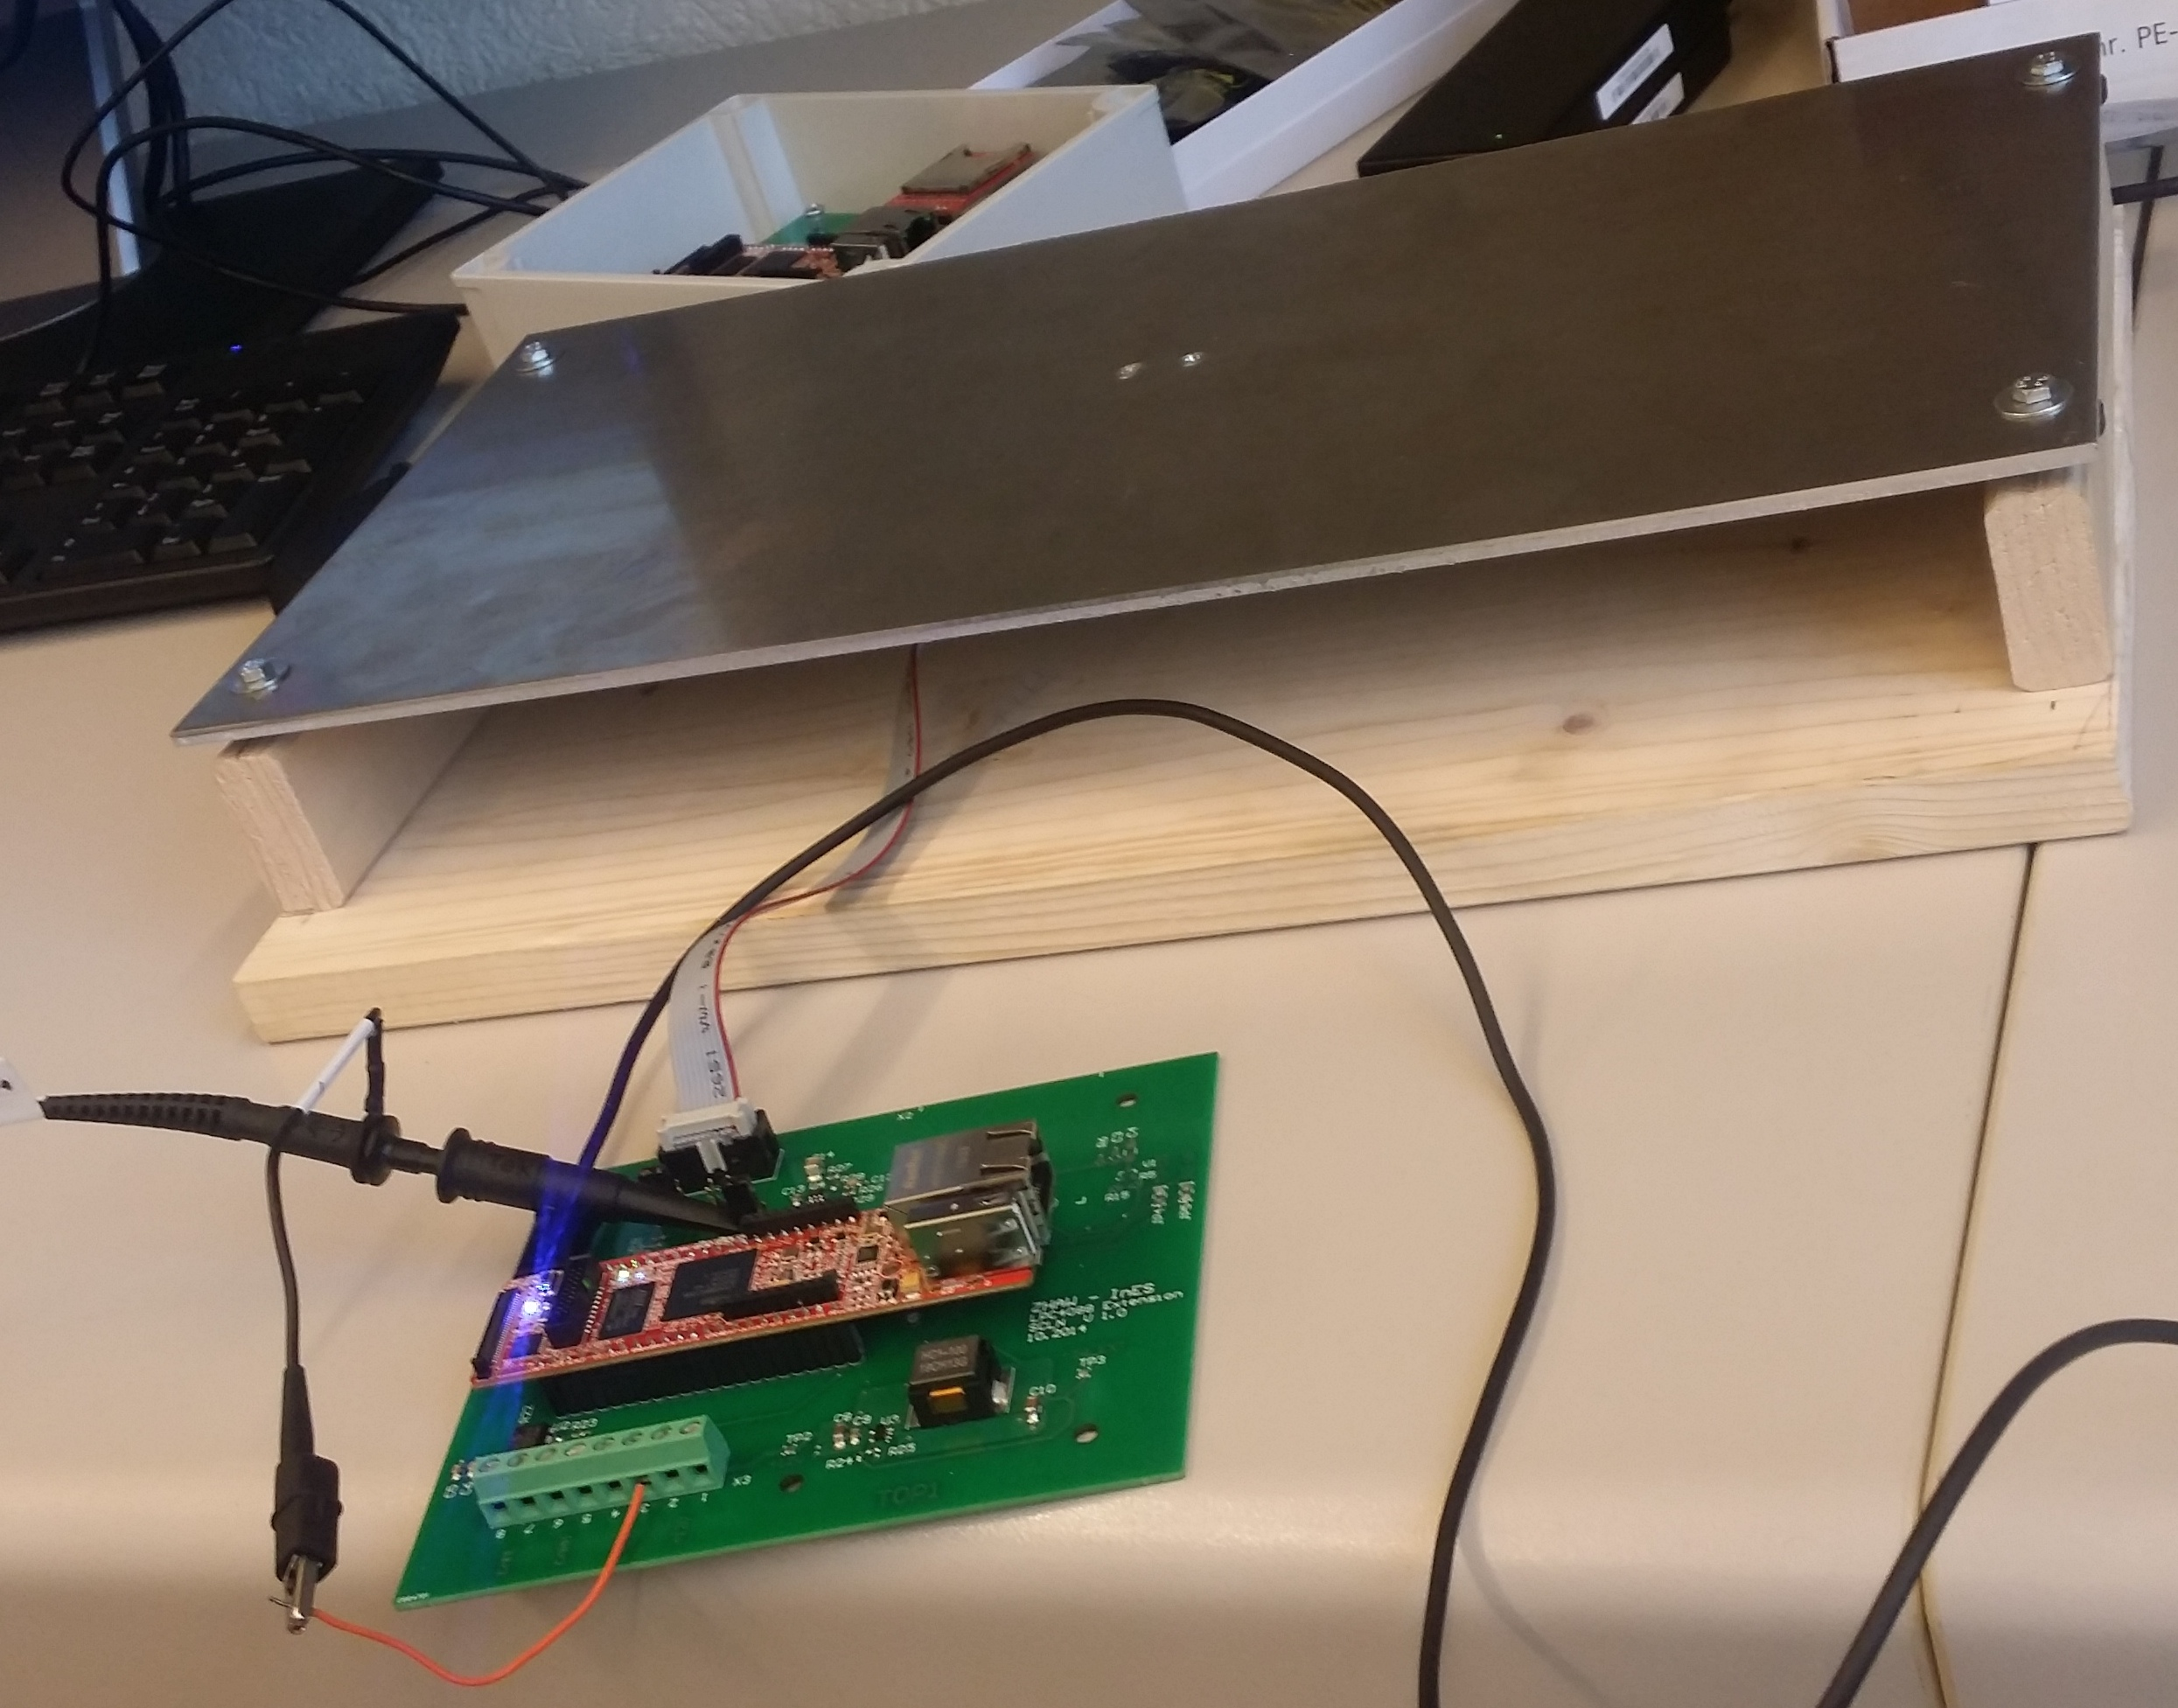
\includegraphics[width=0.8\textwidth]{images/fotos/testaufbau1.jpg}
	\caption{Übersicht des Testaufbaus.}
	\label{fig.testaufbau1}
\end{figure}

\begin{figure}
	\centering
		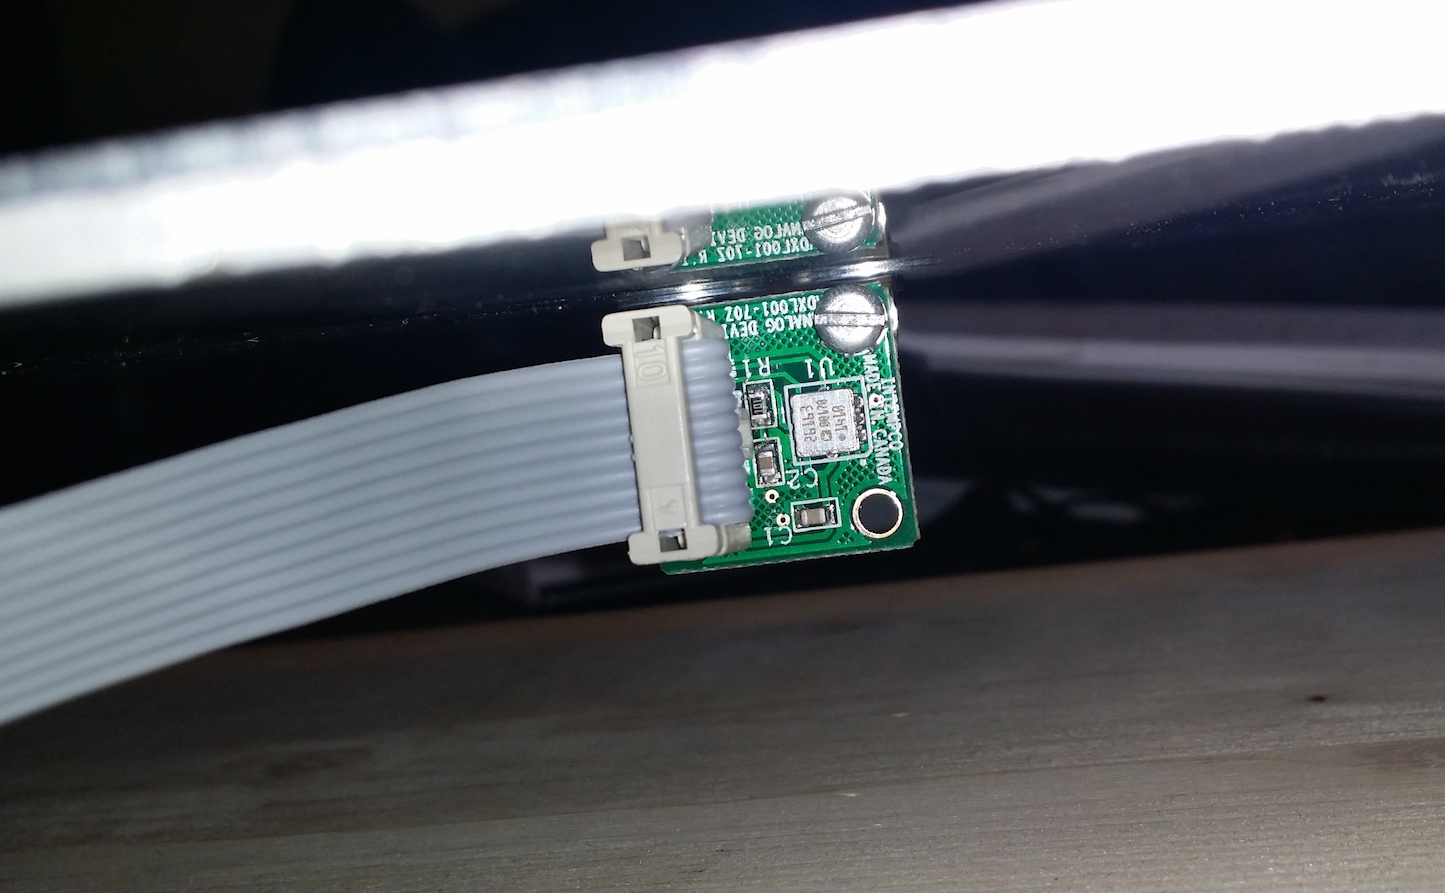
\includegraphics[width=0.8\textwidth]{images/fotos/testaufbau2.jpg}
	\caption{Montage des Sensors im Testaufbau.}
	\label{fig.testaufbau2}
\end{figure}

\section{Datenlogger}
\subsection{T110 Busmaster}
\paragraph{Aktionen} Die Messstation wird an die Stromversorgung angeschlossen.

\paragraph{Resultate} Der \gls{logger} übernimmt die Kontrolle über den CAN-Bus und vergibt jedem angeschlossenen Sensor die eindeutige CAN-ID aus der Konfigurationsdatei.

\paragraph{Testergebnis} Die \glspl{sensoreinh} haben die vordefinierte CAN-ID erhalten. Der Test ist erfüllt.

\subsection{T120 Sensorerkennung}
\paragraph{Aktionen} Eine neue \gls{sensoreinh} wird an die Messstation angeschlossen, deren Seriennummer nicht in der Konfigurationsdatei erfasst ist. Die Messstation wird an die Stromversorgung angeschlossen.

\paragraph{Resultate} Der \gls{logger} erkennt die neue \gls{sensoreinh} und teilt ihr eine eindeutige CAN-ID zu.

\paragraph{Testergebnis} Die \gls{sensoreinh} hat eine bisher unbenutzte, unreservierte CAN-ID erhalten. Der Test ist erfüllt.

\subsection{T130 Uhrzeit}
\paragraph{Aktionen} Die Uhrzeit wird im laufenden Betrieb richtig eingestellt. Die Messstation wird während mind. 12~Stunden in Betrieb gehalten.

\paragraph{Resultate} Die interne Uhrzeit weist nicht mehr als 2~Sekunden Fehlgang innert 12~Stunden auf.

\paragraph{Testergebnis} Bis zur Berichterstellung konnte dieser Test noch nicht durchgeführt werden.

\subsection{T140 Timestamp zurücksetzen}
\paragraph{Aktionen} Über die Konfigurationsschnittstelle wird der Befehl zum Zurücksetzen der \gls{timestamp}s in den \glspl{sensoreinh} gegeben.

\paragraph{Resultate} Alle \glspl{sensoreinh} führen den Befehl innert weniger Sekunden aus und senden ab dann die Ereignisse mit dem neuen \gls{timestamp}.

\paragraph{Testergebnis} Bis zur Berichterstellung konnte dieser Test noch nicht durchgeführt werden.

\subsection{T160 Schnittstelle zum Steuerrechner}
\paragraph{Aktionen} Ein \gls{compi} wird an die Konfigurationsschnittstelle angeschlossen und ein \gls{terminalemu} gestartet.

\paragraph{Resultate} Das Konfigurationsmenü erscheint in der Terminal-Emulation und kann über Tastatureingaben bedient werden.

Die Eingaben werden vom \gls{logger} ausgeführt und bei Bedarf an die \glspl{sensoreinh} kommuniziert.

\paragraph{Testergebnis} Das Konfigurationsmenü funktioniert wie vorgesehen. Die Einstellungen werden an die \glspl{sensoreinh} übertragen.

\subsection{T170 Steuerung Detail-Level}
\paragraph{Aktionen} Am \gls{logger} wird für eine \gls{sensoreinh} ein anderer Detail-Level eingestellt.

\paragraph{Resultate} Die \gls{sensoreinh} wechselt den Detail-Level bei der Übertragung neuer Ereignisse.

\paragraph{Testergebnis} Bis zur Berichterstellung konnte dieser Test noch nicht durchgeführt werden.

\subsection{T180 Daten sammeln und speichern}
\paragraph{Aktionen} Mehrere \glspl{sensoreinh} senden Ereignisdaten an den \gls{logger}. 

\paragraph{Resultate} Der \gls{logger} legt für jede \gls{sensoreinh} eine Datei an und speichert die Ereignisdaten in der richtigen Datei.

\paragraph{Testergebnis} Bis zur Berichterstellung konnte dieser Test noch nicht durchgeführt werden.

\subsection{T190 Tokenvergabe}
\paragraph{Aktionen} Der \gls{logger} vergibt ein Token an eine \gls{sensoreinh}. Nach erhaltenen zehn Nachrichten verfällt der Token. Der \gls{logger} vergibt den Token der nächsten \gls{sensoreinh}.

\paragraph{Resultate} Token wird korrekt weitergegeben. Es sendet nur jene \gls{sensoreinh} Nachrichten, die den Token hält. Die andere \gls{sensoreinh} hält die Ereignisdaten so lange im Zwischenspeicher, bis sie den Token erhält.

\paragraph{Testergebnis} Das Übermittlungsprotokoll des \gls{logger}s und der \glspl{sensoreinh} ist in Listing \ref{t190} aufgeführt und zeigt den korrekten Ablauf des Tests.

\begin{lstlisting}[caption=T190 Tokenvergabe, label=t190]
//Logger                           //Sensor02
// sent Token to Sensor02          // received token
prepare message id: 4020101        Timestamp id  : 2ff0101
OK                                 Token received, start sending 10 msgs

                                   //Sensor03
                                   // no token, stops after timesync
                                   Timestamp id  : 2ff0101

//Logger                           //Sensor02
// receive 10 msgs from Sensor02   // send 10 packages to logger
Sensor data: 055f7cf52602e         Impact complete:
Sensor id  : 1c010201              Starttime: 5633999
Sensor len : 8                     Samples: 46
...                                Peaks: 6
...                                 Maximum: 594
...                                ***********
...                                sent payload 055f7cf52602e
...                                OK, Message sent to logger
...                                
...                                Impact complete:
...                                Starttime: 5829023
...                                Samples: 36
...                                Peaks: 5
...                                Maximum: 260
...                                ***********
...                                sent payload 058f19f45024
Sensor data: 058f19f45024          OK, Message sent to logger
Sensor id  : 1c010201              Token revoked
Sensor len : 8                     
//Logger                           //Sensor03
give token to SensorID 3 of 2      Timestamp id  : 2ff0101
prepare message id: 4030101        Token received, start sending 10 msgs
OK
                                   Impact complete:
                                   Starttime: 11874290
                                   Samples: 1
                                   Peaks: 1
                                   Maximum: 410
                                   ***********
                                   sent payload 0b52ff29a101
Sensor data: 0b52ff29a101          OK, Message sent to logger
Sensor id  : 1c010301              Token revoked
Sensor len : 8                     
                                   Impact complete:
give token to SensorID 2 of 2      Starttime: 12065974
prepare message id: 4020101        Samples: 25
                                   Peaks: 6
                                   Maximum: 334
                                   ***********
                                   sent payload 0b81cb64e6019
                                   No token, message stored
\end{lstlisting}


\section{Sensoreinheit}
\subsection{T400 Konfiguration}
\paragraph{Aktionen} Via Konfigurationsmenü des Datenloggers werden die Parameter des Sensors auf neue Werte gesetzt. 

\paragraph{Resultate} Die \gls{sensoreinh} übernimmt die neuen Einstellungen und passt die Ereigniserkennung entsprechend an.

\paragraph{Testergebnis} Die Konfiguration wurde erfolgreich auf die \gls{sensoreinh} übertragen. Die Konfiguration vor dem Test ist in Listing \ref{t400.1} gegeben, mit der Eingabe 99 werden alle Sensoren ausgewählt. Listings \ref{t400.2} und \ref{t400.3} zeigen, wie der zu konfigurierende Parameter ausgewählt und der neue Wert eingegeben wird. Am \gls{logger} wird im Testmodus das Absenden einer CAN-Nachricht protokolliert, Listing \ref{t400.4}. Die \glspl{sensoreinh} geben im Testmodus ebenfalls eine Bestätigung aus (Listings \ref{t400.5} und \ref{t400.6}), wenn sie eine neue Konfiguration erhalten. Die Änderung des \gls{threshold}s wurde also von beiden Sensoren übernommen.

\begin{lstlisting}[caption=T400 Vorbedingung und Auswahl aller Sensoren, label=t400.1]
Listing sensor config
 Nr  SID  serial    fs  threshold baseline timeout detail     started?
 0)  2  061bfdf6   100        200     2047      30 sparse     started
 1)  3  15117738   100        150     2040      30 peaks only started
 #) Select a sensor from the list.
99) Select all sensors.
 0) cancel
 >
your entry was: 99
\end{lstlisting}

\begin{lstlisting}[caption=T400 Auswahl des Parameters, label=t400.2]
 1) set sampling rate
 2) set threshold value
 3) set baseline value
 4) set timeout
 5) set detail level
 6) start or stop recording
 0) exit
 >
your entry was: 2
\end{lstlisting}

\begin{lstlisting}[caption=T400 Eingabe des neuen \gls{threshold}s, label=t400.3]
 #) Enter threshold value.
baseline + threshold must not exceed 4096
and
baseline - threshold must not be below 0
 0) cancel
 >
your entry was: 250
\end{lstlisting}

\begin{lstlisting}[caption=T400 Sendeprotokoll am \gls{logger}, label=t400.4]
prepare message id: 5020101
OK
prepare message id: 50301001
OK
\end{lstlisting}

\begin{lstlisting}[caption=T400 Konfiguration aus Sensor 3, label=t400.5]
threshold fa   -> geaenderter Wert, von 150 (0x96) auf 250 (0xfa)
fsampling 64   -> wie zuvor, bei 100
timeout 1e     -> wie zuvor, bei 30
baseline 7f8   -> wie zuvor, bei 2040
\end{lstlisting}

\begin{lstlisting}[caption=T400 Konfiguration aus Sensor 2, label=t400.6]
threshold fa   -> geaenderter Wert, von 200 (0xc8) auf 250 (0xfa)
fsampling 64   -> wie zuvor, bei 100
timeout 1e     -> wie zuvor, bei 30
baseline 7ff   -> wie zuvor, bei 2047
\end{lstlisting}


\subsection{T410 Ereignisdetektion}
\paragraph{Aktionen} Die \gls{sensoreinh} ist im Messbetrieb. Am \gls{sensor} wird ein Einschlag simuliert, indem ein Objekt auf die Metallplatte geschlagen wird. 

\paragraph{Resultate} Am Ausgang des \gls{sensor}s misst ein Oszilloskop den Spannungsverlauf. Die so gemessene Referenzkurve wird mit den von der \gls{sensoreinh} ausgegebenen Daten verglichen.

\paragraph{Testergebnis} Die gemessenen Daten decken sich gut. Die vom Oszilloskop ausgegebenen Messdaten sind in der Intensität nicht sehr gut aufgelöst, der Vergleich ist trotzdem möglich. Abbildung \ref{fig.comparison} zeigt in Rot die Messdaten der \gls{sensoreinh}, in Blau die Referenz vom Oszilloskop.

\begin{figure}
	\centering
		
\includegraphics[width=0.8\textwidth]{images/comparison/comparison.png}
	\caption{Vergleich der Messresultate.}
	\label{fig.comparison}
\end{figure}

\subsection{T430 Datenübertragung}
\paragraph{Aktionen} Mehrere Einschläge werden simuliert und mit einem Oszilloskop aufgezeichnet, um Referenzdaten zu haben.

\paragraph{Resultate} Die \gls{sensoreinh} überträgt die Daten von Test T410 fehlerfrei an den \gls{logger}.

\paragraph{Testergebnis} Bis zur Berichterstellung konnte dieser Test noch nicht durchgeführt werden.

\subsection{T450 Rohdatenaufzeichnung}
\paragraph{Aktionen} Eine \gls{sensoreinh} wird in den Rohdatenmodus versetzt.

\paragraph{Resultate} Die \gls{sensoreinh} zeichnet Rohdaten während 60 Sekunden ohne einen Puffer-Überlauf auf und überträgt die Daten an den \gls{logger}.

\paragraph{Testergebnis} Bis zur Berichterstellung konnte dieser Test noch nicht durchgeführt werden.

\section{Nichtfunktionale Tests}
\subsection{T710 Stromverbrauch}
\paragraph{Aktionen} Der Stromverbrauch der Messanlage mit dem \gls{logger} und drei \glspl{sensoreinh} wird gemessen. 

\paragraph{Resultate} Der Stromverbrauch sollte unter 3~Watt liegen.

\paragraph{Testergebnis} Ein \gls{logger} und zwei \gls{sensoreinh} haben einen Stromverbrauch von 
%% !TeX spellcheck = de_CH
%%%%%%%%%%%%%%%%%%%%%%%%%%%%%%%%%%%%%%%%%%%%%%%%%%%%%%%%%%%%%%%%%
%  _____   ____  _____                                          %
% |_   _| /  __||  __ \    Institute of Computitional Physics   %
%   | |  |  /   | |__) |   Zuercher Hochschule Winterthur       %
%   | |  | (    |  ___/    (University of Applied Sciences)     %
%  _| |_ |  \__ | |        8401 Winterthur, Switzerland         %
% |_____| \____||_|                                             %
%%%%%%%%%%%%%%%%%%%%%%%%%%%%%%%%%%%%%%%%%%%%%%%%%%%%%%%%%%%%%%%%%
%
% Project     : BA Welti Keller
% Title       : 
% File        : grundlagen.tex Rev. 00
% Date        : 15.09.2014
% Author      : Tobias Welti
%
%%%%%%%%%%%%%%%%%%%%%%%%%%%%%%%%%%%%%%%%%%%%%%%%%%%%%%%%%%%%%%%%%

% Kapitel rausgenommen

\chapter{Grundlagen}\label{chap.grundlagen}
\todo{Grundlagen: entweder aus anderen Kapiteln zusammentragen oder das Kapitel streichen}
\todo{etwas über signalerfassung, (aufwand hilbert etc.), mems?}
% !TeX spellcheck = de_CH
%%%%%%%%%%%%%%%%%%%%%%%%%%%%%%%%%%%%%%%%%%%%%%%%%%%%%%%%%%%%%%%%%
%  _____   ____  _____                                          %
% |_   _| /  __||  __ \    Institute of Computitional Physics   %
%   | |  |  /   | |__) |   Zuercher Hochschule Winterthur       %
%   | |  | (    |  ___/    (University of Applied Sciences)     %
%  _| |_ |  \__ | |        8401 Winterthur, Switzerland         %
% |_____| \____||_|                                             %
%%%%%%%%%%%%%%%%%%%%%%%%%%%%%%%%%%%%%%%%%%%%%%%%%%%%%%%%%%%%%%%%%
%
% Project     : BA Welti Keller
% Title       : 
% File        : hardware.tex Rev. 00
% Date        : 15.09.2014
% Author      : Tobias Welti
%
%%%%%%%%%%%%%%%%%%%%%%%%%%%%%%%%%%%%%%%%%%%%%%%%%%%%%%%%%%%%%%%%%

\chapter{Hardware-Konzept}\label{chap.hardware}



\section{Hardware-Architektur}\label{sec.hw_arch}

Anhand der funktionalen Vorgaben für die Messstation werden der \gls{logger}, die \gls{sensoreinh} und das Bussytem im folgenden genauer spezifiziert und die Komponenten ausgewählt.

\subsection{Datenlogger}
Der \gls{logger} sammelt die Daten der \glspl{sensoreinh} über das \gls{bussys} ein und speichert sie ab. Dafür benötigt er das \gls{bussys}, einen Mikroprozessor, internen Speicher und ein leicht auswechselbares Speichermedium. Ausserdem soll über eine Schnittstelle ein Computer angeschlossen werden können, um den Betrieb der Messstation zu steuern. Der \gls{logger} wird in einem wasserdichten Gehäuse untergebracht. Für den Austausch des Speichermediums wäre eine verschraubbare Öffnung denkbar.

\begin{figure}[H]
	\centering
		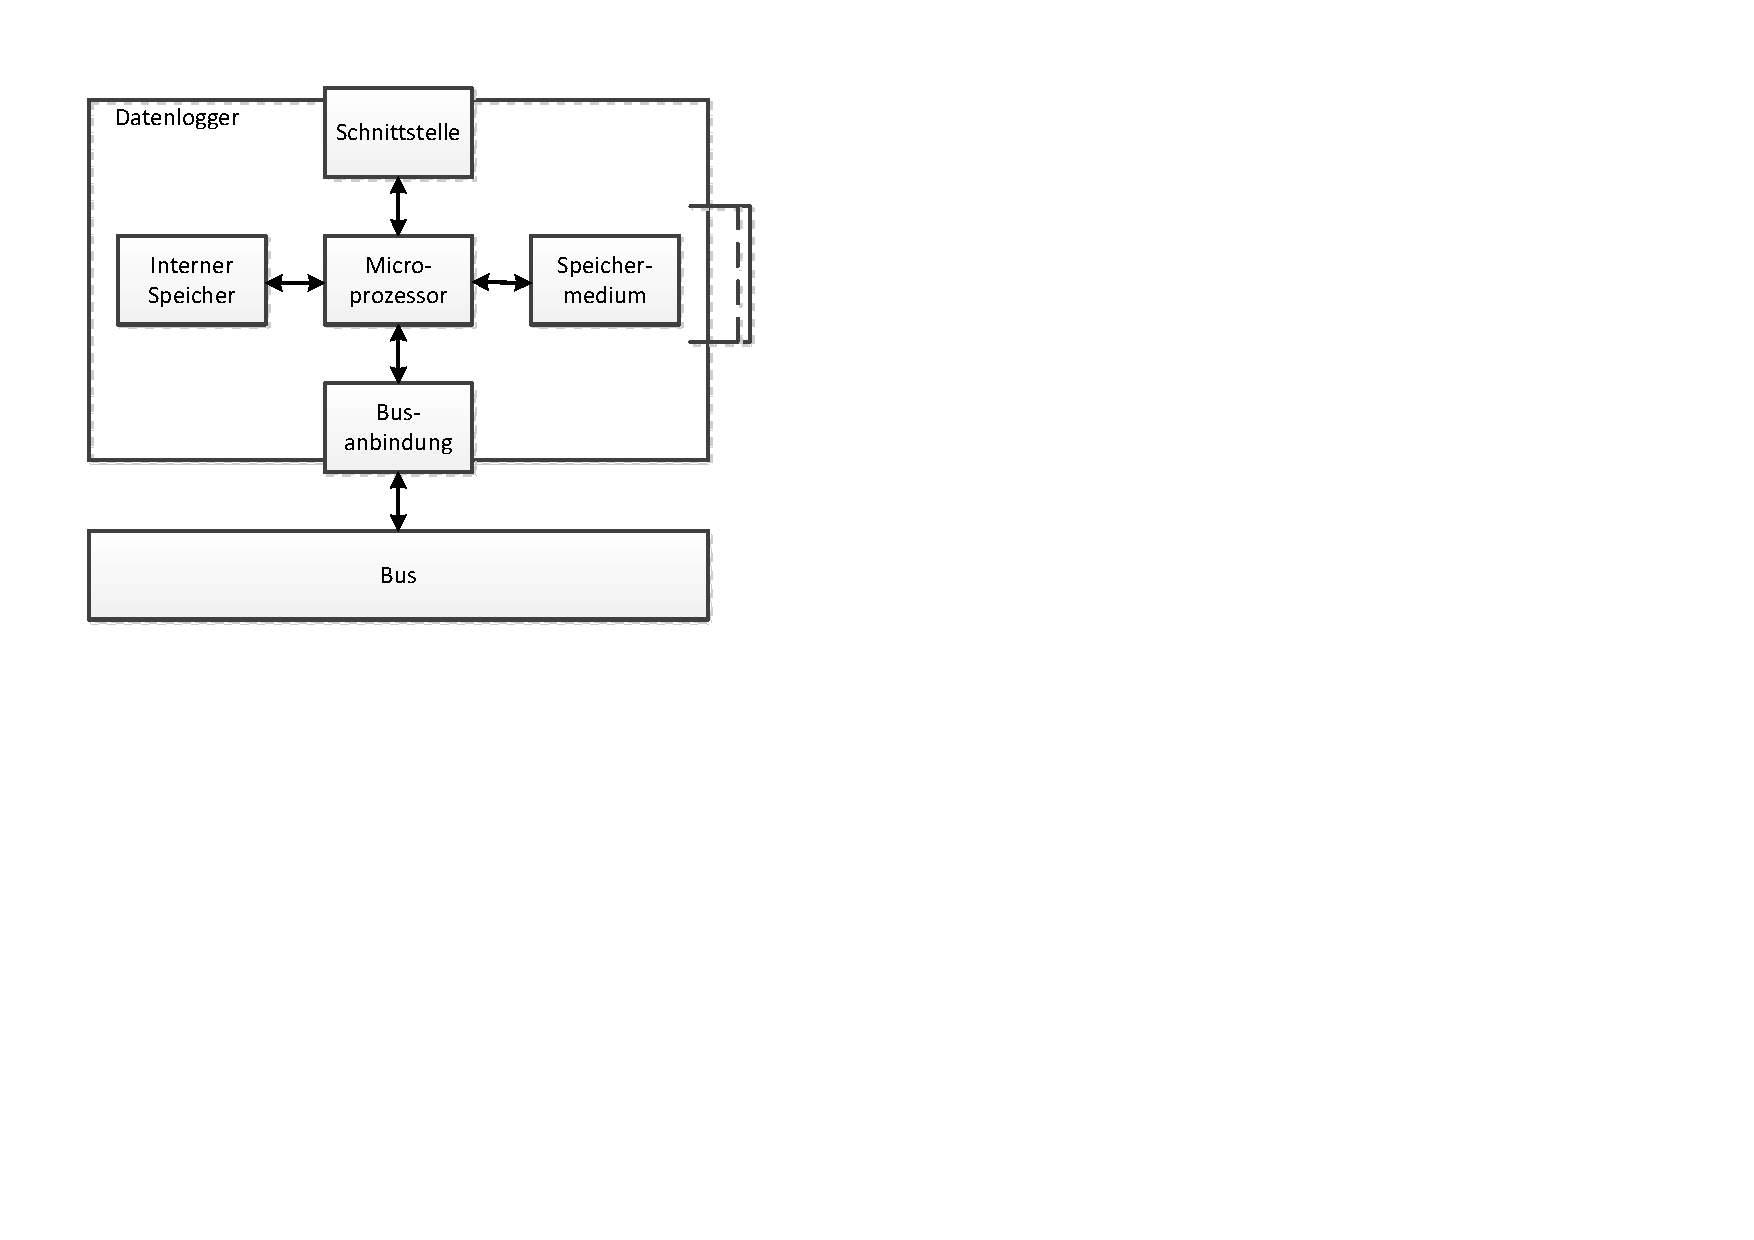
\includegraphics[width=0.8\textwidth]{images/visio/hardwarekonzept_logger.pdf}
	\caption{Hardwarekonzept des \gls{logger}s.}
	\label{fig.hwkonzept_logger}
\end{figure}

\subsection{Sensoreinheit}
Die \gls{sensoreinh} benötigt einen Beschleunigungssensor, um die Einschläge von Geschiebe zu messen. Über einen Analog-Digital-Wandler (ADC) werden die Messsignale digitalisiert. Die gemessenen Signale werden von einem Mikroprozessor verarbeitet, im internen Speicher zwischengespeichert und über das \gls{bussys} an den \gls{logger} übertragen.

\begin{figure}[H]
	\centering
		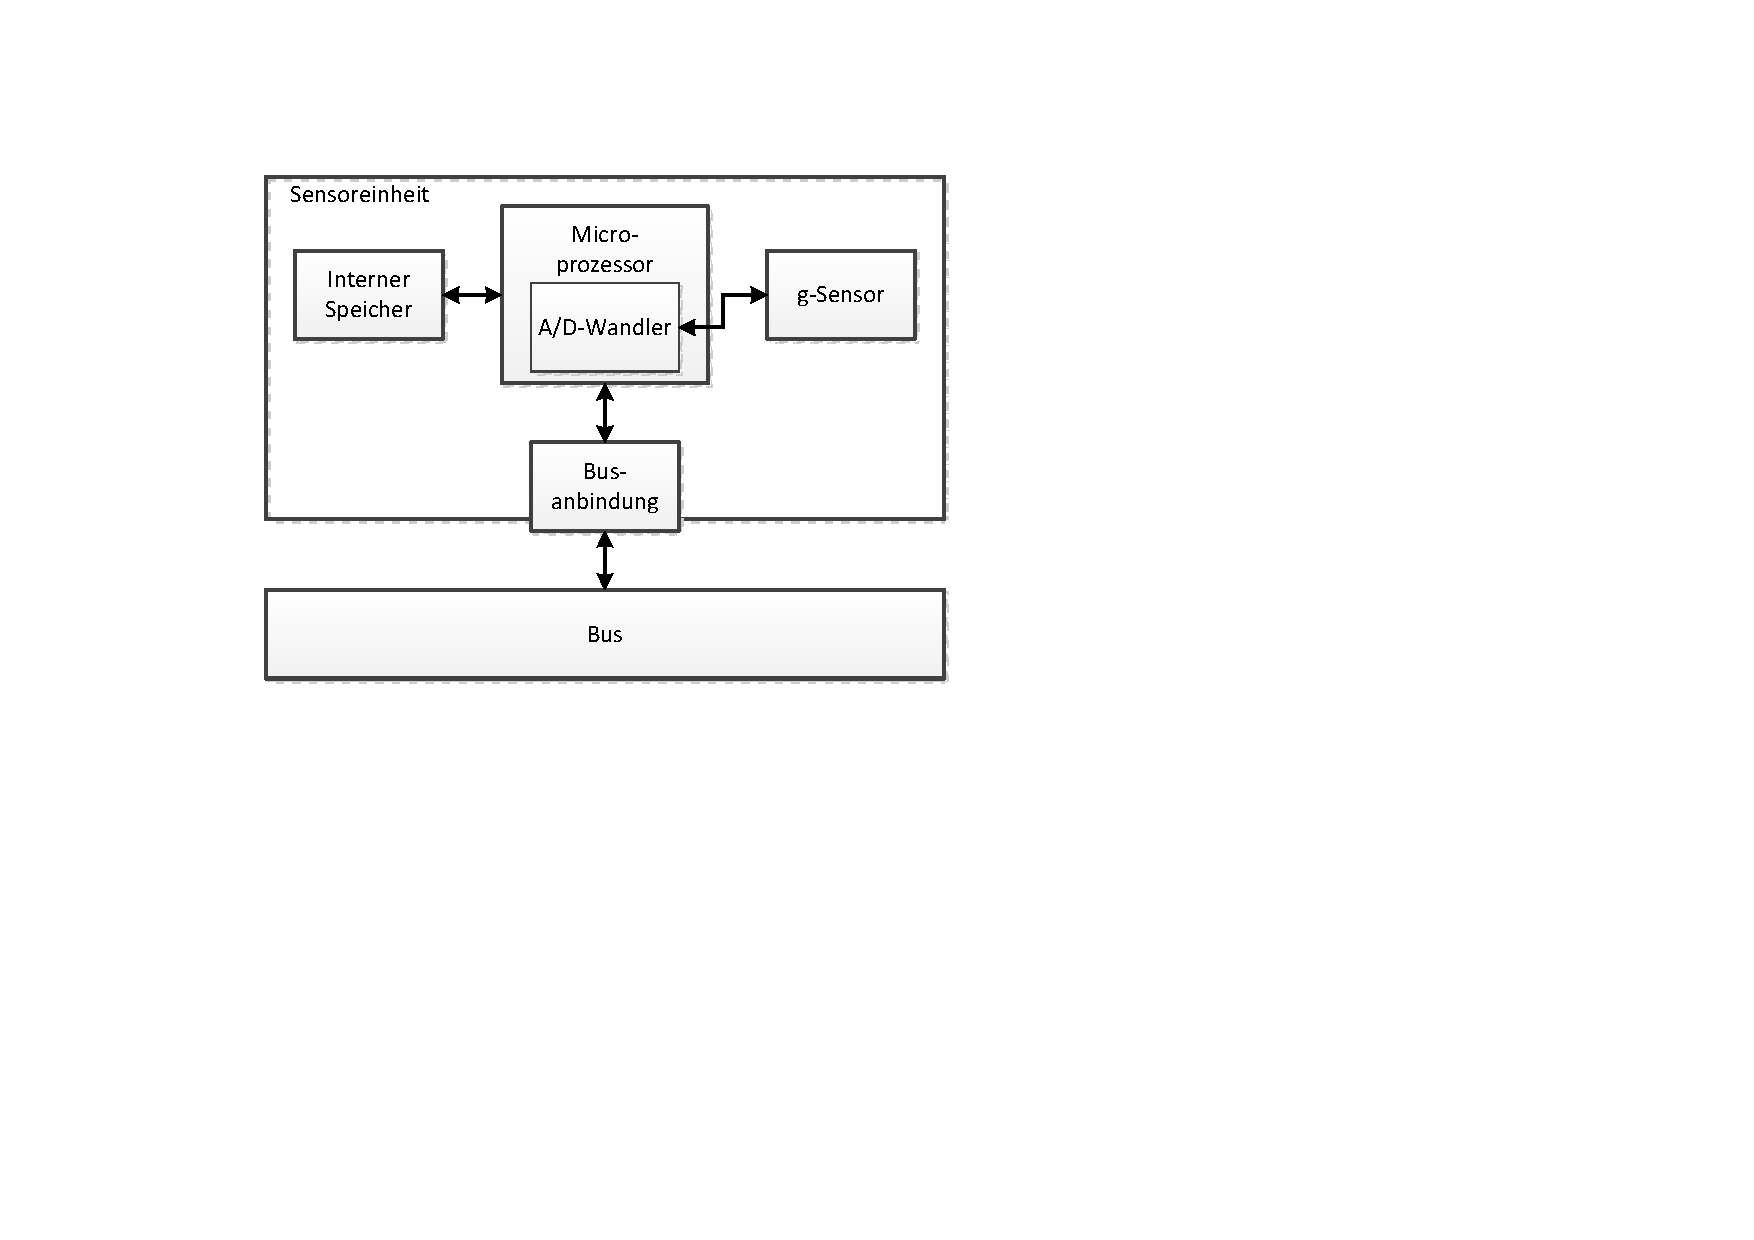
\includegraphics[width=0.8\textwidth]{images/visio/hardwarekonzept_sensor.pdf}
	\caption{Hardwarekonzept der \gls{sensoreinh}.}
	\label{fig.hwkonzept_sensor}
\end{figure}

\subsection{\gls{bussys}}
Das \gls{bussys} muss die Daten und Befehle zwischen \gls{logger} und \glspl{sensoreinh} übertragen. Die Reichweite des \gls{bussys}s muss genügen, um alle Komponenten der Messinstallation zu verbinden. Die Datenbandbreite muss die Übertragung der Messresultate aller \glspl{sensor} erlauben.


\section{Komponentenauswahl}

\subsection{Mikroprozessor}
Bei der Auswahl des Mikroprozessors werden folgende Kriterien berücksichtigt:

\begin{itemize}
\item Rechenleistung genügend für allfällige zusätzliche Anforderungen.
\item Analog-Digital-Wandler mit genügender Abtastrate und Auflösung.
\item Digitaler Signal Prozessor integriert für die Verarbeitung der Messdaten.
\item Ein-/Ausgänge für das \gls{bussys}.
\item Ein-/Ausgänge für den externen Speicher.
\item möglichst geringer Stromverbrauch.
\end{itemize}

\todo{Tabelle verschiedener uCs zum Vergleich}

\subsection{Bus-System}
Anhand folgender Kriterien wurde ein \gls{bussys} ausgewählt:

\begin{itemize}
\item Übertragungsbandbreite genügend für fortlaufende Übertragung von Rohdaten einer \gls{sensoreinh}.
\item Reichweite mindestens 20 Meter.
\item Robust gegenüber äusseren Einflüssen.
\item Mindestens zwanzig Busteilnehmer möglich.
\end{itemize}

\begin{table}
\begin{tabular}{|l|l|l|l|l|}
\hline  & \textbf{Bitrate}      & \textbf{Distanz} & \textbf{Clients} & \textbf{Besonderheiten}\\ 
\hline \textbf{CAN} & \begin{minipage}{2cm}
1 MBit/s\\ 125 kBit/s
\end{minipage} & \begin{minipage}{1.5cm}40 m\\500 m\end{minipage} & > 20 & \begin{minipage}{6cm}
\mbox{ }\\+ Collision Detection (CD) umgehen mit Polling durch Master.\\
+ Bei synchronem CAN wird CD durch ID gelöst.\\
+ CAN Controller sendet Interrupt Request bei erhaltener Nachricht.\\
\end{minipage} \\ 
\hline \textbf{SPI} & ..100 MBit/s & < 1 m & \begin{minipage}{1cm}
slave select
\end{minipage} & \begin{minipage}{6cm}
\mbox{ }\\- Pro Client eine Slave Select Leitung\\
- Daisy Chain $\Rightarrow $alle MC beschäftigt.\\
- Bei Ausfall eines MC ganzer Bus unterbrochen.\\
\end{minipage} \\ 
\hline \textbf{RS485} & \begin{minipage}{2cm}
35 MBit/s\\100 kBit/s
\end{minipage} & \begin{minipage}{1.5cm}
10 m\\1200 m
\end{minipage} & >32 & \begin{minipage}{6cm}
\mbox{ }\\- Master am besten in der Mitte des Bus $\Rightarrow$ ungünstig.\\
- Braucht 2..4 Drähte (bei Full Duplex)\\
- braucht pull-up und pull-down Widerstände $\Rightarrow$ mehr Leistungsaufnahme.\\
\end{minipage} \\ 
\hline \textbf{Ethernet} & 100 MBit/s & 100 m & > 20 & \begin{minipage}{6cm}
\mbox{ }\\+ Stromversorgung bei Power over Ethernet (PoE) integriert.\\
- kein Bus sondern allenfalls Daisychain.\\
- bei Daisychain kein PoE möglich.\\
\end{minipage} \\ 
\hline \textbf{Feldbus} &  &  &  & \begin{minipage}{6cm}
\mbox{ }\\ist eine Familie von Bussen, z.B. CAN-Bus\\
\end{minipage} \\ 
\hline \textbf{I2C} & 0.4..5 Mbit/s & wenige Meter & < 20 & \begin{minipage}{6cm}
\mbox{ }\\nur für kurze Distanzen, Bitrate nimmt rasch ab.\\
\end{minipage}\\
\hline 
\end{tabular}
\caption{Entscheidungsmatrix für die Auswahl des \gls{bussys}s.}
\label{table.bussystem}
\end{table} 

In Tabelle \ref{table.bussystem} sind die Eigenschaften diverser \glspl{bussys} aufgeführt.

\paragraph{Kommentare}
SPI und I2C sind nur für kurze Distanzen geeignet und sind deshalb keine Option.
Die Verwendung von Ethernet zur Datenübertragung würde zwei Schnittstellen auf jeder \gls{sensoreinh} voraussetzen, um die \glspl{sensor} hintereinander zusammenzuhängen (Daisychain). Jedes Paket müsste vom Microcontroller weitergeleitet werden, wenn es für einen anderen Empfänger bestimmt ist. Dies führte zu einer zusätzlichen Belastung der Microcontroller. Stromversorgung über Ethernet ist mit PowerOverEthernet (PoE) zwar möglich, erfordert aber spezielle Geräte zur Speisung über den Stecker des Datenkabels. Dies verunmöglicht eine Daisychain mit PoE, neben dem Datenkabel wäre noch ein Kabel für die Stromversorgung notwendig.

\paragraph{Vergleich CAN-Bus und RS485}
\todo{Kriterienliste RS485/CAN einfügen, Lit-Referenz auf White Paper von IXXAT}
CAN und RS: Stecker nicht definiert => wasserdichte Stecker einfach zu finden.

\paragraph{Entscheidung}
CAN-Bus erfüllt alle Kriterien und erlaubt es, den Busmaster am Ende des Bus zu platzieren. Dies ist ein Vorteil gegenüber RS485, wo der Master in der Mitte platziert werden sollte. CAN-Bus bietet bereits Kollisionserkennung und Fehlererkennung, während dies bei RS485 in der Software gelöst werden muss. Für CAN-Bus sind Bus-Treiber (Transceiver) erhältlich, die mit hohen Spannungen umgehen können, was das \gls{bussys} robuster gegenüber Umwelteinflüssen macht. Die Grösse der Datenpakete ist bei CAN-Bus auf 8 Byte begrenzt, bei RS485 werden die Datenpakete über die Software frei definiert, was ein klarer Vorteil von RS485 darstellt. Insgesamt überwiegen die Vorteile von CAN-Bus klar. 



\subsection{Speichermedium}
\paragraph{Kriterien} Das externe Speichermedium soll möglichst klein sein, wenig Stromverbrauch haben und einfach auswechselbar sein. Bei Inaktivität sollte das Medium wenn möglich keinen Strom verbrauchen. Für einen mehrwöchigen unabhängigen Betrieb einer Messstation muss genügend Speicherkapazität bereitgestellt werden.

\paragraph{Datenmenge} Pro \gls{sensor} werden bei hohem Geschiebeaufkommen maximal hundert \glspl{ereignis} pro Sekunde erwartet. Ein solches Geschiebeaufkommen stellt jedoch die Ausnahme dar. Ein \gls{ereignis} benötigt je nach verlangtem Detailgrad und Dauer des \gls{ereignis}ses 10..90 Byte Speicherplatz. Für den normalen Betriebsmodus werden 50 Byte/\gls{ereignis} gerechnet, bei 5 \glspl{ereignis}n pro Sekunde. Damit ergibt sich eine Datenrate von 250 Byte/s, die es pro \gls{sensor} abzuspeichern gilt. Mit zehn \glspl{sensor} im Einsatz müssen 2.5 kByte/s gespeichert werden. 

\paragraph{Unabhängige Betriebsdauer} Pro Gigabyte Speicherplatz können 111 Stunden Daten für zehn \glspl{sensor} gespeichert werden. Bei hohem Geschiebeaufkommen mit zwanzig mal mehr \glspl{ereignis}n bleiben immer noch 5 Stunden Aufzeichnungszeit pro Gigabyte. Begnügt man sich mit weniger Details, reichen fallen pro \gls{sensor} in zehn Sekunden rund 400 Byte Daten an. Bei dieser Datenrate reicht ein Gigabyte für rund 700 Stunden. Auch bei hohem Geschiebeaufkommen kann die Anlage mehrere Tage an Daten speichern. 

\paragraph{Kapazität} Heute sind Speichermedien mit Kapazitäten bis über 128 GB erhältlich, so dass die Detailrate kein entscheidendes Kriterium mehr darstellt.

\paragraph{Datentransfer} Für den Transfer der Daten aus dem \gls{logger} auf einen Computer gibt es grundsätzlich zwei Varianten. Entweder man liest die Daten über eine Schnittstelle auf den Computer aus, oder man tauscht das Speichermedium aus. Das Auslesen via Schnittstelle benötigt zusätzlich Strom, das Wechseln des Speichermediums setzt einen mehr oder weniger komfortablen und trotzdem wasserdichten Zugang zum Medium voraus. Da heute Speichermedien mit kleinem Platzbedarf erhältlich sind, könnte ein solcher Zugang recht einfach mit einem Schraubverschluss realisiert werden.

\paragraph{Vergleich} In Tabelle \ref{table.speichermedium} werden verschiedene Speichermedien miteinander verglichen. In der Spalte 'Breite' ist aufgelistet, wie gross eine Öffnung mindestens sein muss, um das Speichermedium wechseln zu können. 'Pins' gibt an, wie viele Leitungen für den Anschluss des Mediums am Microcontroller nötig sind. Der Stromverbrauch in Klammern ist für den Standby-Modus des Speichermediums.

\begin{table}
\begin{tabular}{|l|l|l|l|l|}
	\hline
	                      & \textbf{Breite} & \textbf{Pins} & \textbf{Stromverbrauch} & \textbf{Bemerkungen}        \\ \hline
	\textbf{SD-Card}      & 24 mm           & 9             & 20..100 mA (0.2 mA)     & 4 bit breiter serieller Bus \\ \hline
	\textbf{CompactFlash} & 43 mm           & 50            & max. 70 mA (k.A.)       & paralleler Bus              \\ \hline
	\textbf{USB-Stick}    & min. 12 mm      & 4             & typ. 70 mA (k.A.) &  \\ \hline
\end{tabular} 
\caption{Entscheidungsmatrix zur Auswahl des Speichermediums.}
\label{table.speichermedium}
\end{table} 

\todo{Literatur-Referenzen in Tabelle \ref{table.speichermedium}}


\paragraph{Entscheid} Für einen verschraubbaren Verschluss ist die CompactFlash-Karte zu breit, das Gehäuse würde dadurch sehr gross werden. Die SD-Karte und der USB-Stick sind vergleichbar in der Grösse. Von der SD-Karte sind auch kleinere Varianten erhältlich. Eine Öffnung für den Austausch des Speichermediums kann eine gewisse Grösse ohnehin nicht unterschreiten, damit hineingegriffen werden kann. Da die SD-Karte im Standby den geringeren Stromverbrauch hat, wird der \gls{logger} mit einem SD-Kartenleser ausgestattet.

\subsection{Sensor}
\todo{Sensorauswahl beschreiben}

\subsection{Schnittstelle}
\todo{Schnittstellenauswahl beschreiben}



\section{Komponenten}
\todo{Texten}
\subsection{Cortex M4 Mikroprozessor}

\todo{Texten}
\subsubsection{Flash Speicher}

\todo{Texten}
\subsubsection{SDRAM}

\todo{Texten}

\subsection{Beschleunigungs-Sensor}

\todo{Texten}
\subsection{CAN Bus}

\todo{Texten}
\subsubsection{CAN Transceiver}

\todo{Texten}

\subsection{SD Karte}

\todo{Texten}
\subsection{UART Schnittstelle}

\todo{Texten}
\section{\gls{logger}}

\todo{Texten}
\begin{figure}[H]
	\centering
		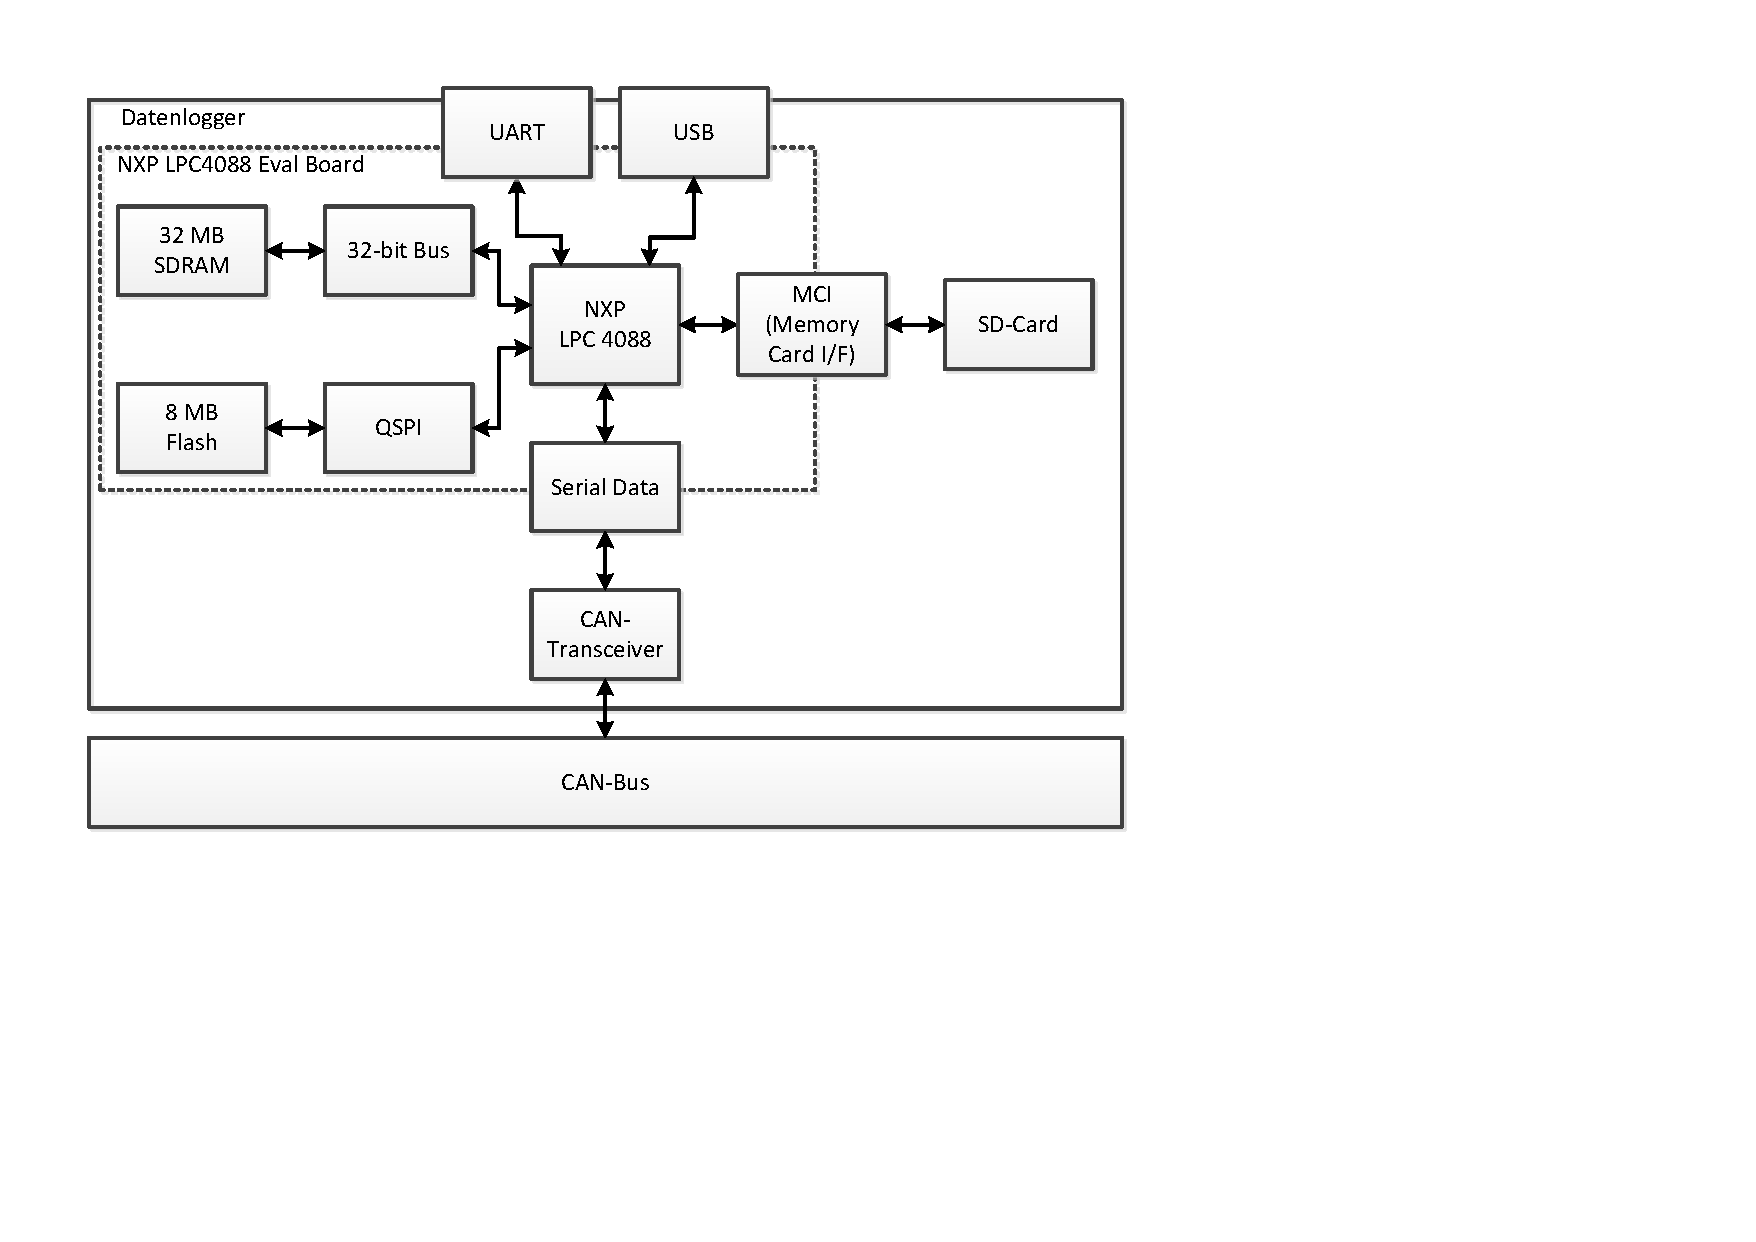
\includegraphics[width=0.8\textwidth]{images/visio/hardware_logger.pdf}
	\caption{Schematischer Hardware-Aufbau des \gls{logger}s.}
	\label{fig.hw_logger}
\end{figure}



\section{Sensoreinheit}

\todo{Texten}
\begin{figure}[H]
	\centering
		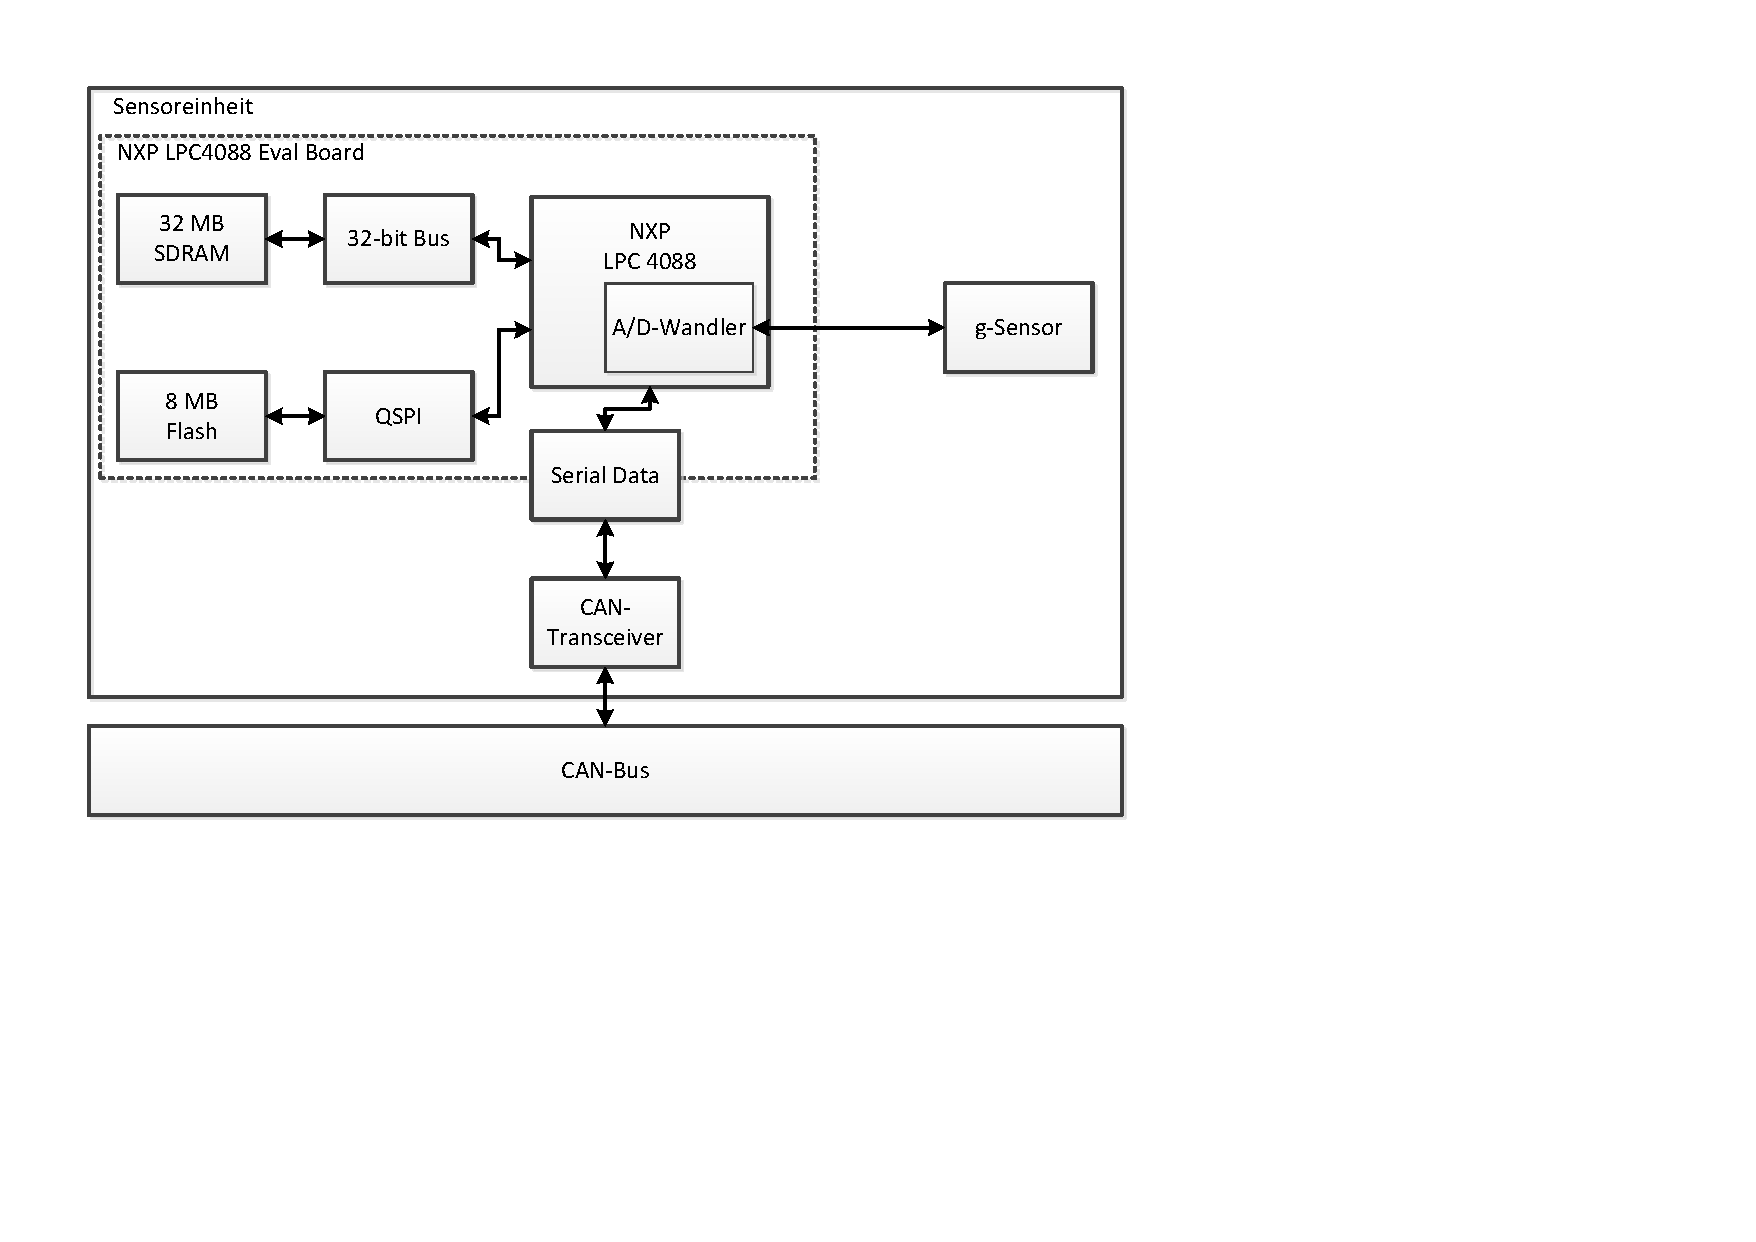
\includegraphics[width=0.8\textwidth]{images/visio/hardware_sensor.pdf}
	\caption{Schematischer Hardware-Aufbau der \gls{sensoreinh}.}
	\label{fig.hw_sensor}
\end{figure}



% !TeX spellcheck = de_CH
%%%%%%%%%%%%%%%%%%%%%%%%%%%%%%%%%%%%%%%%%%%%%%%%%%%%%%%%%%%%%%%%%
%  _____   ____  _____                                          %
% |_   _| /  __||  __ \    Institute of Computitional Physics   %
%   | |  |  /   | |__) |   Zuercher Hochschule Winterthur       %
%   | |  | (    |  ___/    (University of Applied Sciences)     %
%  _| |_ |  \__ | |        8401 Winterthur, Switzerland         %
% |_____| \____||_|                                             %
%%%%%%%%%%%%%%%%%%%%%%%%%%%%%%%%%%%%%%%%%%%%%%%%%%%%%%%%%%%%%%%%%
%
% Project     : BA Welti Keller
% Title       : 
% File        : software.tex Rev. 00
% Date        : 15.09.2014
% Author      : Tobias Welti
%
%%%%%%%%%%%%%%%%%%%%%%%%%%%%%%%%%%%%%%%%%%%%%%%%%%%%%%%%%%%%%%%%%

\chapter{Software-Konzept}\label{chap.software}


\section{Software-Stack}\label{sec.sw_stack}
\todo{Glossar: Impact, Bus, Mikroprozessor, A/D-Wandler, Pin, Sensor, Threshold/Grenzwert, }

\subsection{Überblick}\label{subsec.sw_ueberblick}

\begin{figure}[H]
	\centering
		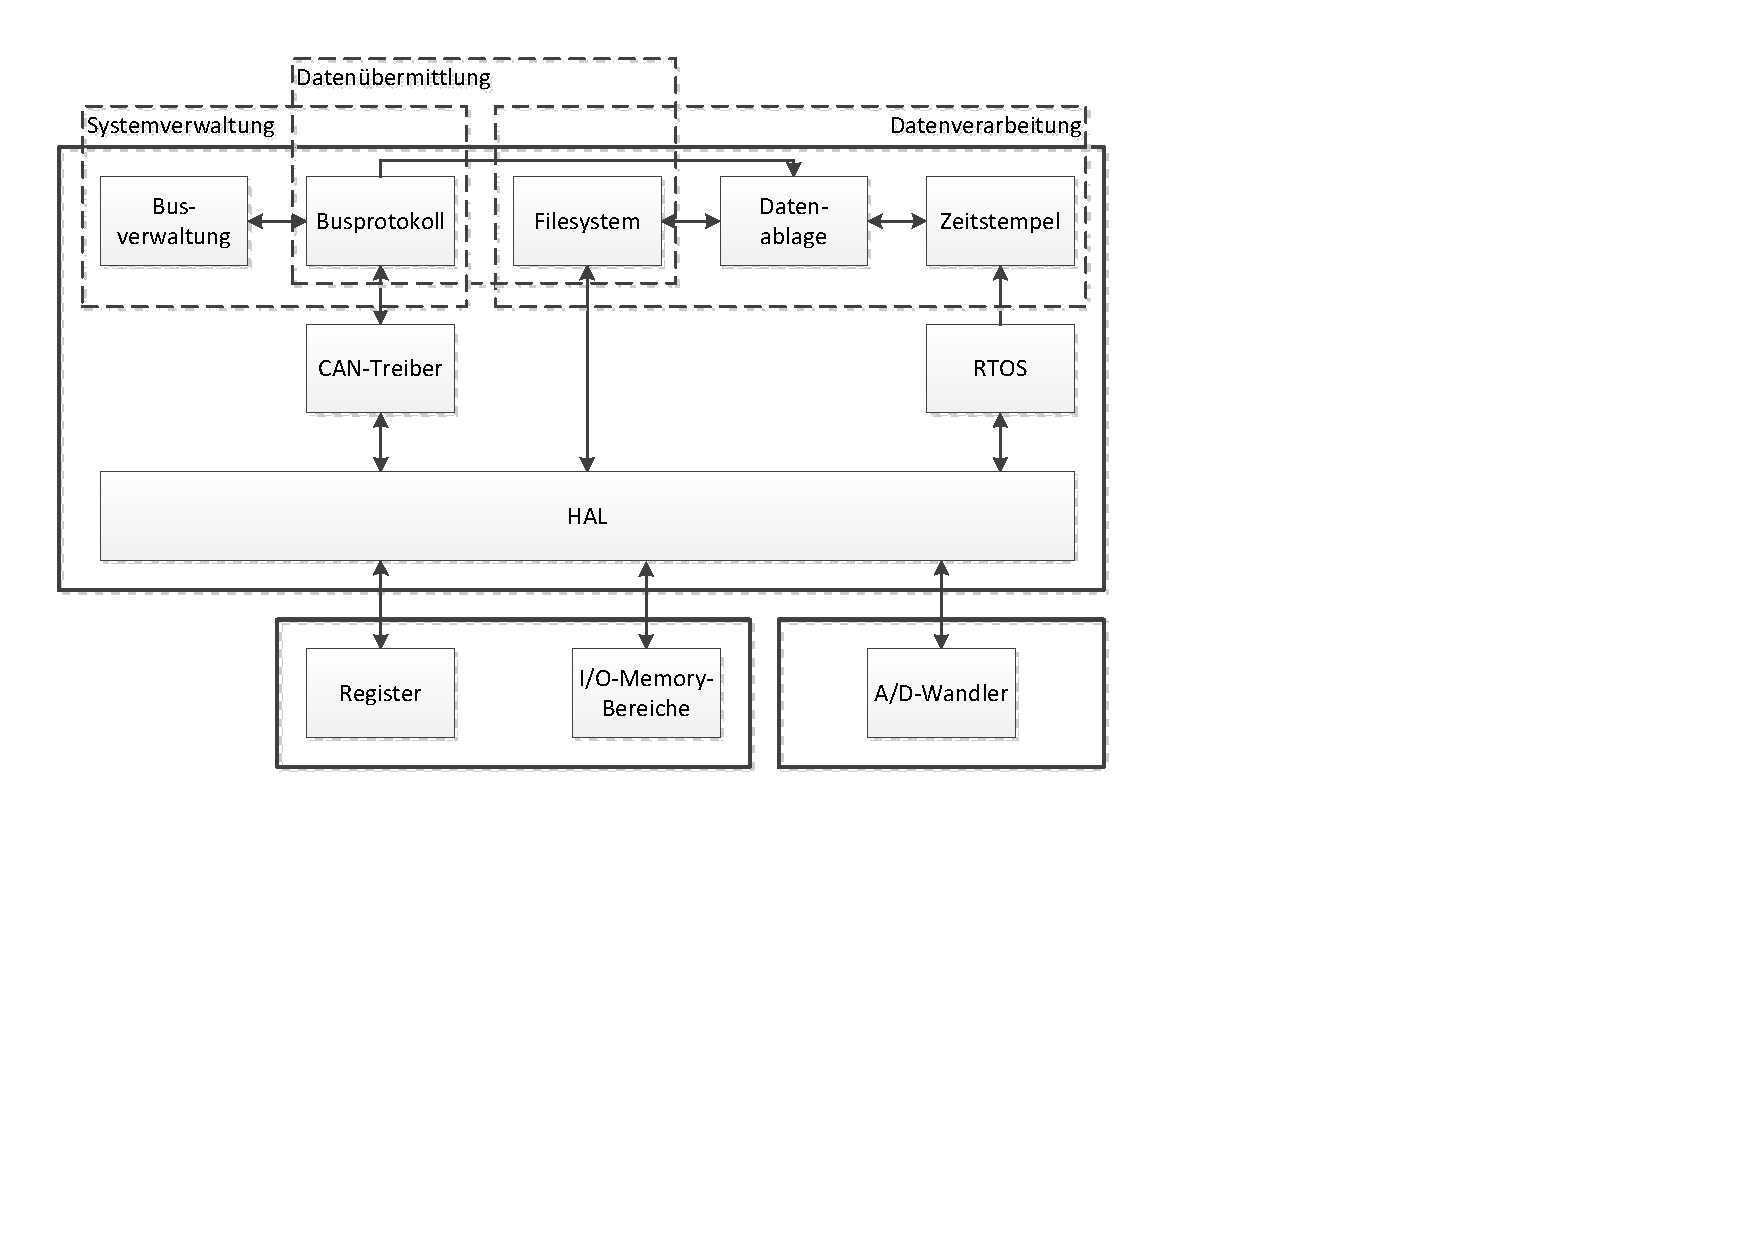
\includegraphics[width=0.8\textwidth]{images/visio/Softwarestack_Logger.pdf}
	\caption{Softwarestack des Datenloggers.}
	\label{fig.sw_logger}
\end{figure}

\begin{figure}[H]
	\centering
		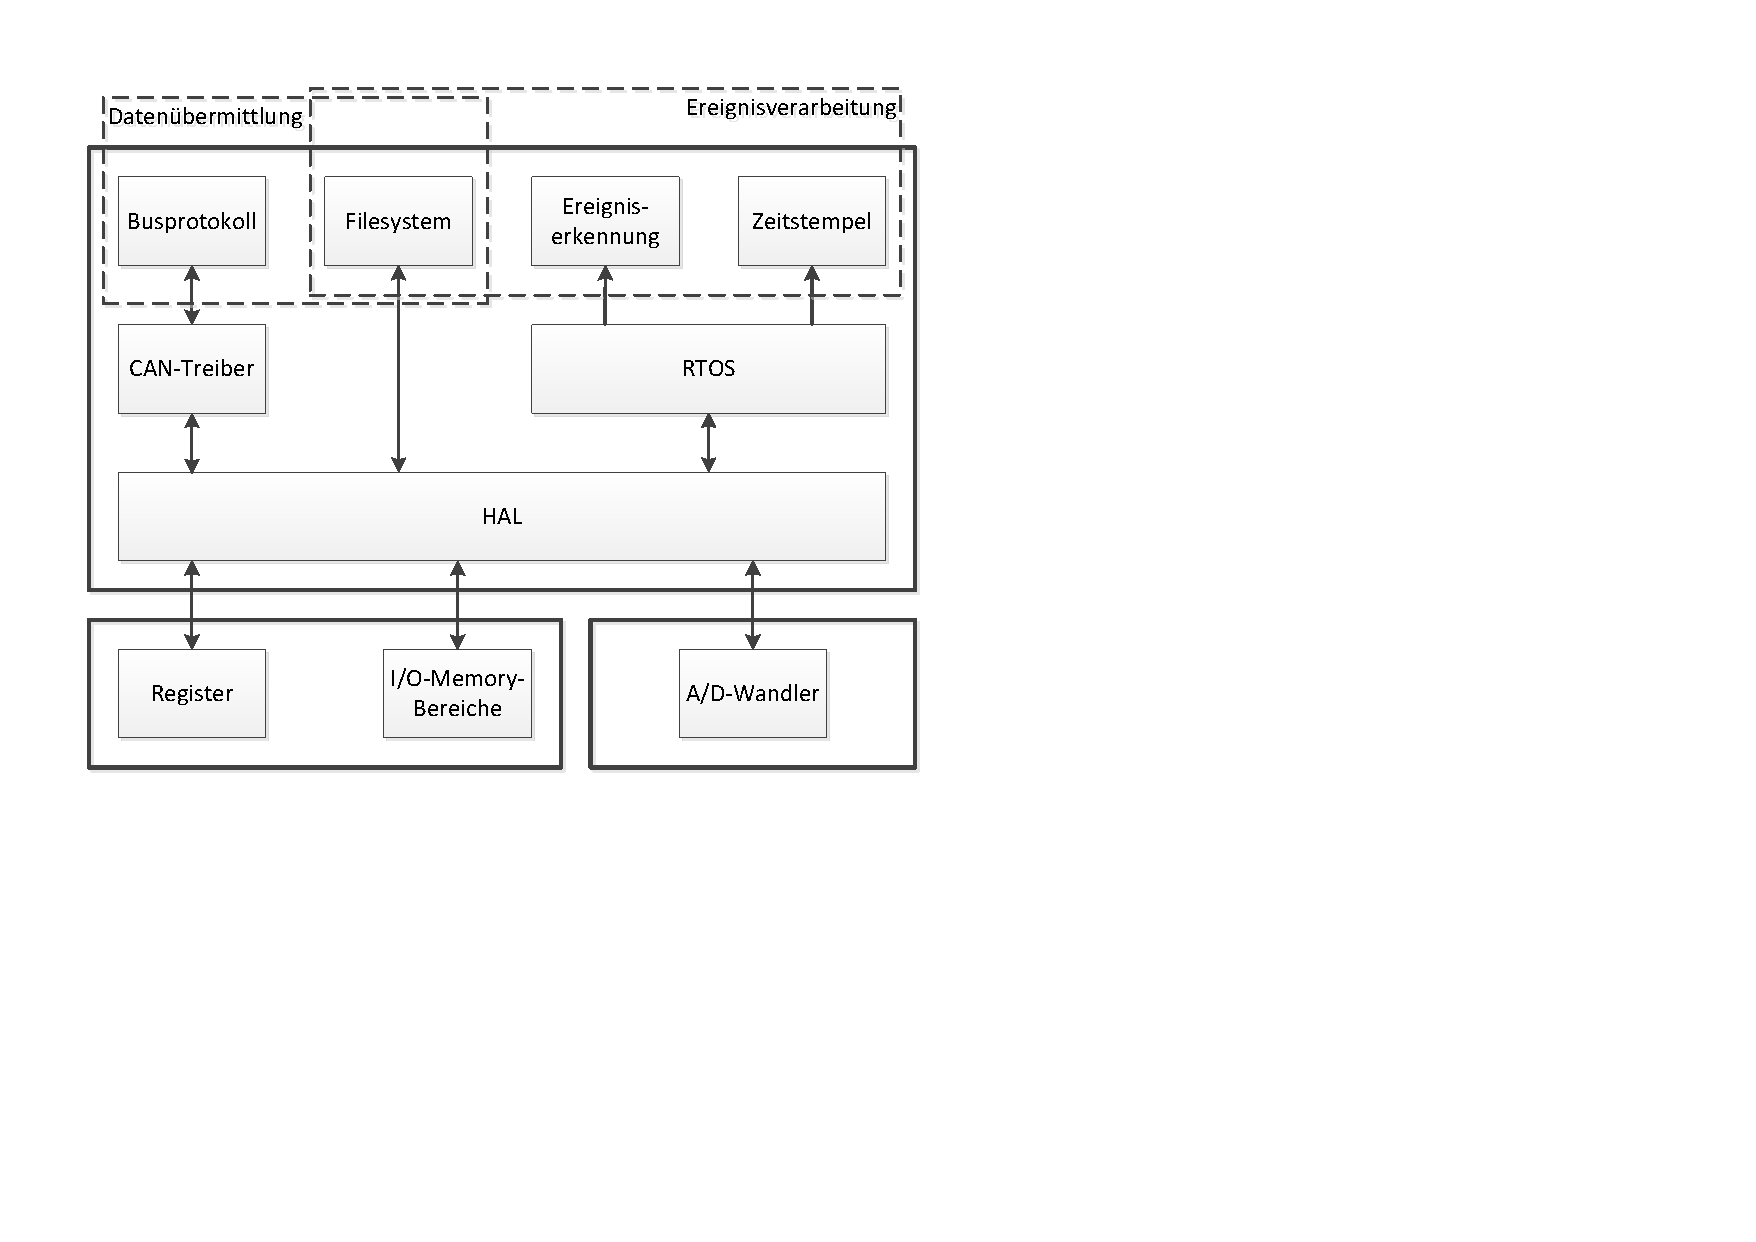
\includegraphics[width=0.8\textwidth]{images/visio/Softwarestack_Sensor.pdf}
	\caption{Softwarestack der Sensoreinheit.}
	\label{fig.sw_sensor}
\end{figure}



\subsection{Messdatenerfassung}\label{subsec.sw_messen}
Der NXP LPC4088 Mikroprozessor verfügt über einen 12-bit A/D-Wandler, der über einen Multiplexer auf acht Pins messen kann. Auf dem verwendeten Quickstart-Board stehen 6 Pins für A/D-Wandlung zur Verfügung. Für die geplante Anwendung reicht ein A/D-Eingang, da der Beschleunigungs-Sensor die Beschleunigung nur auf einer Achse misst. Der A/D-Wandler des NXP LPC4088 wird mit einer Abtastrate von 10~kHz betrieben. Falls höhere Abtastraten nötig sind, kann der A/D-Wandler mit bis zu 400~kHz betrieben werden.



\subsection{Ereigniserkennung}\label{subsec.sw_ereignis}
Vom WSL wurde die Ereigniserkennung bisher mittels Hilbert-Transformation gelöst. Die Hilbert-Transformation liefert die umhüllende Kurve des gemessenen Signals. Überschreitet die Umhüllende den Threshold, markiert dies den Start eines neuen Ereignisses. Fällt die Umhüllende unter den Threshold, ist das Ereignis beendet. Um den Rechenaufwand der Hilbert-Transformation zu umgehen, lösen wir die Ereigniserkennung einfacher.
\todo{FSM-figur anpassen auf neue Stati}
\begin{figure}[H]
	\centering
		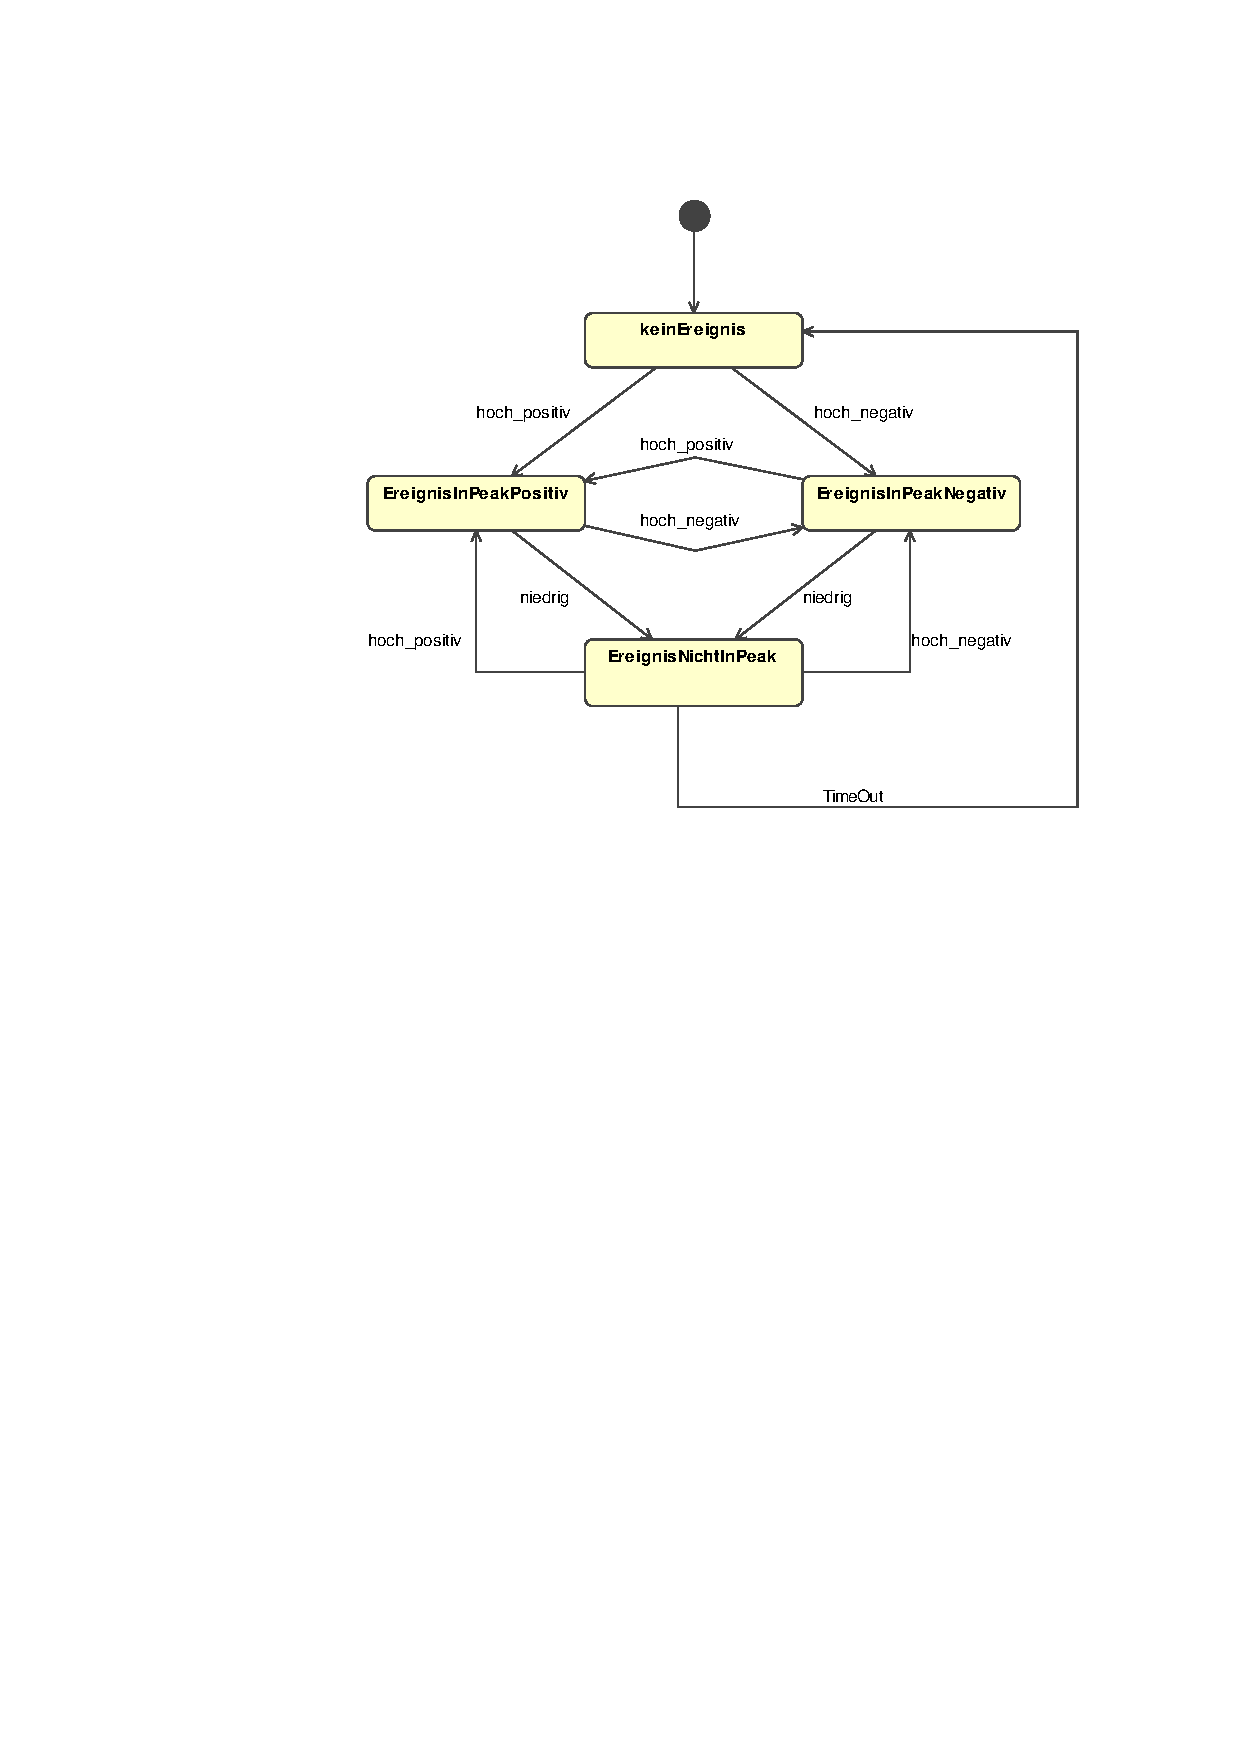
\includegraphics[width=0.6\textwidth]{images/magicdraw/Ereigniserkennung.pdf}
	\caption{Zustandsmaschine der Ereigniserkennung.}
	\label{fig.fsm_impact_detection}
\end{figure}

\todo{Ereigniserkennung beschreiben, welche Parameter können konfiguriert werden}
\todo{Zusammenhänge A/D-Wandlung und Ereigniserkennung und Übertragung beschreiben}
\todo{Verschiedene Betriebsmodi mit Grafiken beschreiben}
\todo{Berechnungen, in welchem Modus wie lange gemessen werden kann, und wie lange ein Sensor mit dem vorhandenen Speicher die Resultate zwischenspeichern kann. Allenfalls ein System erwähnen, das automatisch zwischen verschiedenen Modi hin- und herschalten kann. (Ist allerdings heikel). Wie viele Sensoren können in welchem Modus gleichzeitig am System betrieben werden, bei welcher Ereignisrate ist Schluss mit Busbandbreite.}

\subsection{Timestamp}\label{subsec.sw_timestamp}
\todo{Timestamp beschreiben, Rechnung über die Dauer der eindeutigen Zuweisung.}

\subsection{Verwaltung der Messstation}\label{subsec.sw_busverwaltung}
\todo{Busverwaltung beschreiben}

\begin{figure}[H]
	\centering
		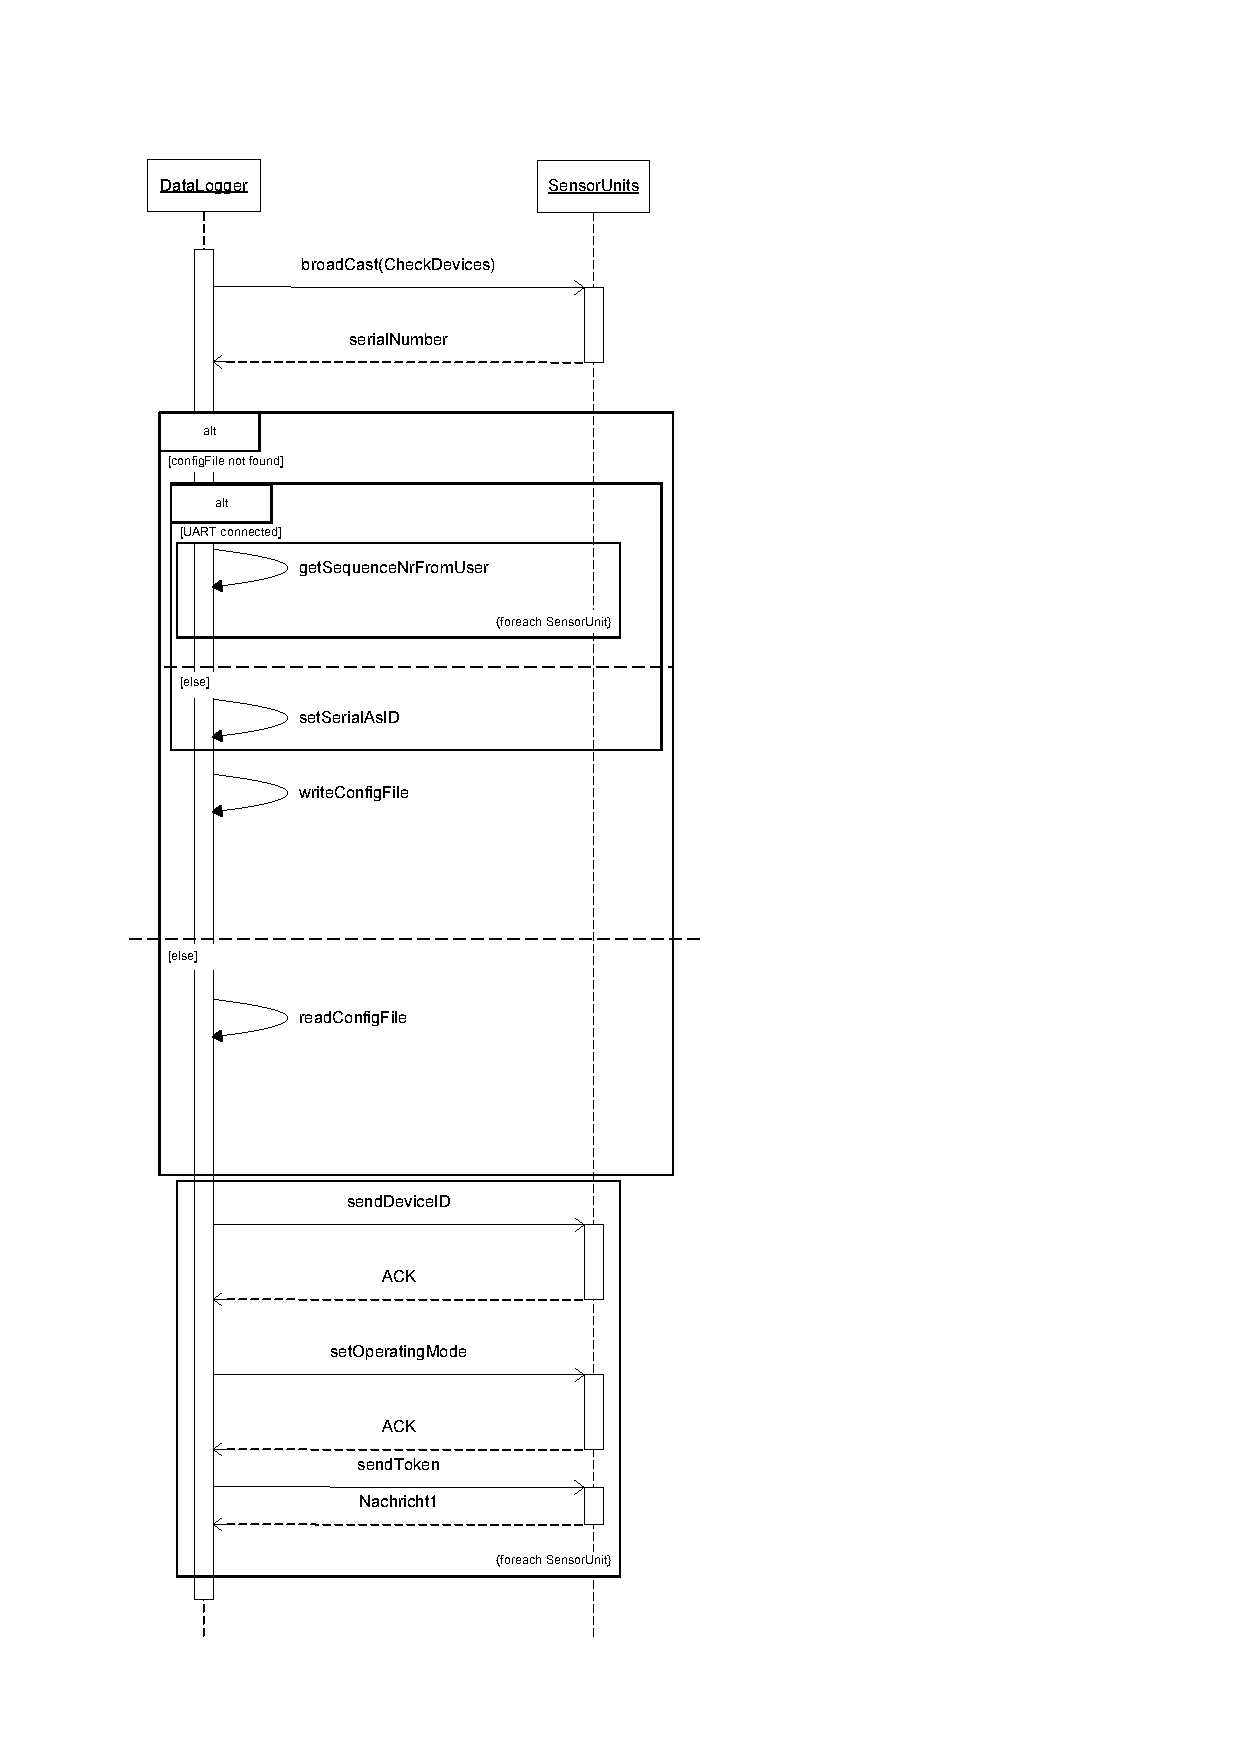
\includegraphics[height=0.9\textheight]{images/magicdraw/StartUpSequenz.pdf}
	\caption{Sequenzdiagramm des Startupvorgangs der Messstation.}
	\label{fig.seq_startup}
\end{figure}

\todo{Figur \ref{fig.seq_startup} aufteilen auf zwei Seiten. (PDF-crop)}

\subsection{Busprotokoll}\label{subsec.sw_busprotokoll}
\todo{Busprotokoll austüfteln. Darstellung siehe HW-Konzept Rioxo, genaue Beschreibung der Nachrichtentypen. Timestamp der einzelnen Peaks bezieht sich auf Offset vom Beginn des Impacts.}
\todo{Kommunikationsdiagramm Bushandler}
\todo{Interrupt-System des Bushandlers aufführen}

\subsection{Filesystem}\label{subsec.sw_filesystem}
\todo{Texten}
\todo{Frage: wird für jeden Sensor ein eigenes File geführt? Kann man alle Files offen lassen oder ist das keine gute Idee? Was ist besser, jedes mal das File-Ende zu suchen um neues anzuhängen?}

\subsection{UART-Kommandozeile}\label{subsec.sw_uart}
\todo{Dokumentation über die Kommandos, wird später für die Bedienungsanleitung gebraucht}

\section{Funktionalität}\label{sec.sw_funktionalitaet}
\todo{Texten}

\section{Konfiguration}\label{sec.sw_konfiguration}
\todo{Hier eine Art Bedienungsanleitung zur Konfiguration geben. Welches Kommando hat was 
zur Folge? (Wird Datenerfassung neu gestartet, werden allenfalls andere Sensoren deaktiviert 
etc.}
% !TeX spellcheck = de_CH
%%%%%%%%%%%%%%%%%%%%%%%%%%%%%%%%%%%%%%%%%%%%%%%%%%%%%%%%%%%%%%%%%
%  _____   ____  _____                                          %
% |_   _| /  __||  __ \    Institute of Computitional Physics   %
%   | |  |  /   | |__) |   Zuercher Hochschule Winterthur       %
%   | |  | (    |  ___/    (University of Applied Sciences)     %
%  _| |_ |  \__ | |        8401 Winterthur, Switzerland         %
% |_____| \____||_|                                             %
%%%%%%%%%%%%%%%%%%%%%%%%%%%%%%%%%%%%%%%%%%%%%%%%%%%%%%%%%%%%%%%%%
%
% Project     : BA Welti Keller
% Title       : 
% File        : resultate.tex Rev. 00
% Date        : 15.09.2014
% Author      : Tobias Welti
%
%%%%%%%%%%%%%%%%%%%%%%%%%%%%%%%%%%%%%%%%%%%%%%%%%%%%%%%%%%%%%%%%%

\chapter{Resultate}\label{chap.resultate}

\section{Testfälle}
Die wichtigsten Testfälle für die grundsätzliche Funktionalität der Messstation konnten erfolgreich abgeschlossen werden. Für einige Tests blieb jedoch nicht genügend Zeit vor der Fertigstellung des Berichts. Diese Tests werden so weit möglich noch nachgeholt.

Im Kapitel \ref{chap.tests} ab Seite \pageref{chap.tests} sind die Testfälle und die Testergebnisse aufgeführt.


Zum Zeitpunkt des Verfassens dieses Berichts konnten keine weiteren Tests durchgeführt werden. Geplant währen

\section{Ereigniserkennung}
Der \gls{adwandler} des \emph{NXP LPC4088} \gls{mc} wurde wie geplant in Betrieb genommen und liefert Messdaten, die sich sehr gut mit dem analogen Ausgangssignal des \gls{sensor}s decken. Abbildung \ref{fig.comparison} zeigt den Vergleich zwischen der Messung von Oszilloskop (blau) und der \gls{sensoreinh} (grün). Die \gls{sensoreinh} arbeitete mit einer \gls{fs} von 10000~\ensuremath{Hz}, das Oszilloskop zeichnete mit einer \gls{fs} von 3.125~MHz auf. Um ein Ereignis zu simulieren, wurde ein Golfball auf den Testaufbau (siehe im Verzeichnis Fotos/Testaufbau/ auf der beiliegenden CD) fallen gelassen. Der Vergleich zeigt, dass die beiden Kurven gut übereinstimmen. 

\begin{figure}
	\centering
		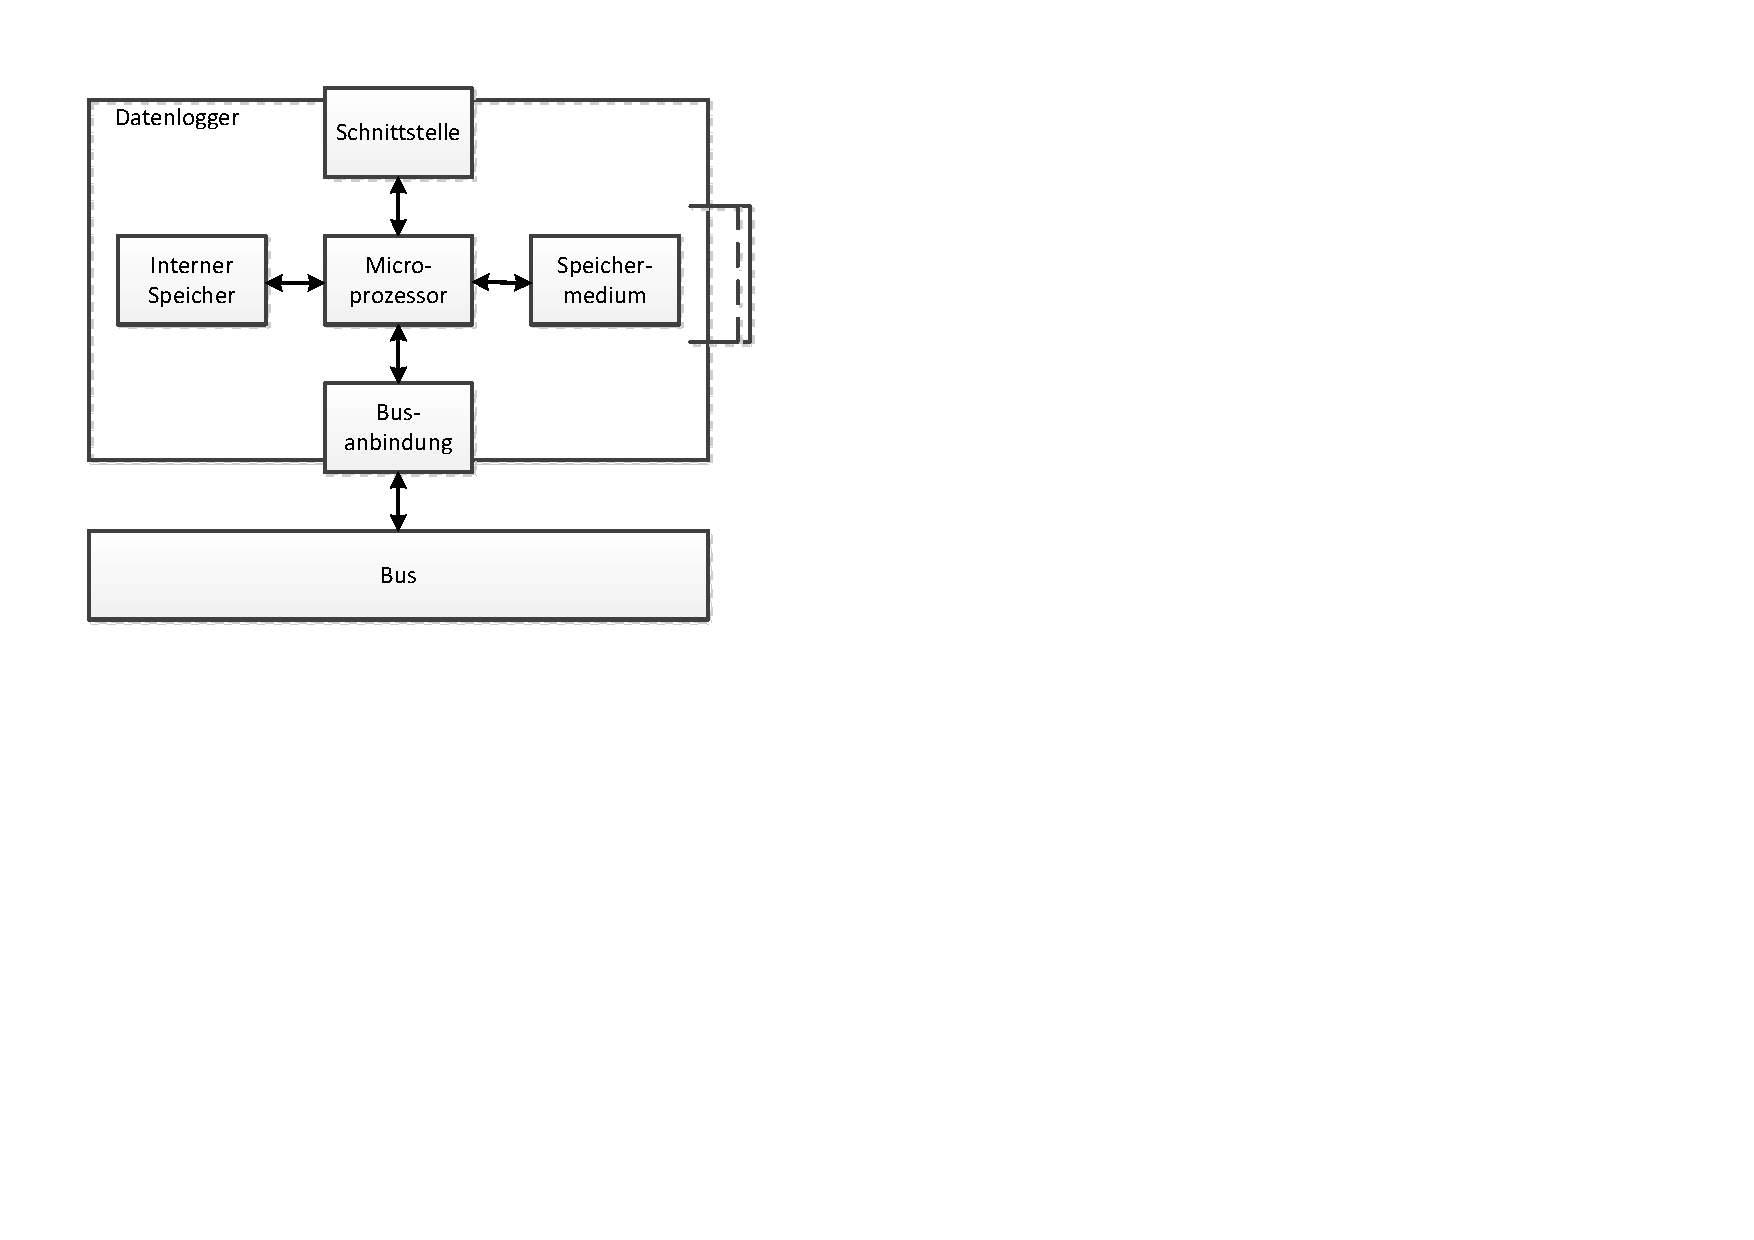
\includegraphics[width=0.8\textwidth]{images/visio/hardwarekonzept_logger.pdf}
	\caption{Vergleichsmessung mit Oszilloskop und \gls{sensoreinh}.}
	\label{fig.comparison}
\end{figure}


Der Betrieb mit 10000~Hz war für unseren Testaufbau genügend, die Peaks traten mit einer Frequenz von ungefähr 2000~Hz auf. Die Frequenz der Peakspitzen variiert sowohl mit der Plattenkonstruktion als auch mit der Korngrösse, Kornbeschaffenheit und der Art des Aufschlags. Daher muss für den tatsächlichen Messbetrieb eine Kalibrierung gemacht werden, um die geeigneten Parameter zu finden.

Für Versuche mit verschiedenen \gls{fs} blieb keine Zeit mehr. So können wir zur Zeit nicht sagen, was die höchstmögliche \gls{fs} mit der aktuellen Software ist.

\section{Daten-Reduktion und -Speicherung}
Die Datenreduktion durch Wahl der verschiedenen Detail-Level ist effizient gelöst und sehr effektiv. Pro Messwert müssen lediglich zwei Vergleiche für die Bestimmung des Signalpegels gemacht werden, sowie zwei Vergleiche mit je einem vorhergehenden Wert für die Bestimmung des Peak-Maximums und des Ereignis-Maximums.

Die Wahl des Detail-Levels beeinflusst lediglich, welche Daten übertragen werden. Auf die Zwischenspeicherung hat sie keinen Einfluss. Vor und nach der Übertragung finden keine komplexen Umrechnungen an den Messdaten statt. Die \gls{bitbreite} wird von 12 Bit auf 8 Bit reduziert. Die grösste Datenreduktion erfolgt durch die Auswahl der relevanten Daten.

\subsection{Rohdaten (raw)}
Es werden alle Messpunkte übertragen und gespeichert. Es findet keine Datenreduktion statt. Pro Messpunkt fällt 1 Byte an. Bei einer \gls{fs} von 10000~Hz resultiert ein Datenstrom von 10000~Byte/s.

\subsection{Detaillierte Ereignisdaten (detailed)}
Es werden nur die Messpunkte der Ereignisse gespeichert. Messpunkte, die nicht zu einem Ereignis gehören, werden verworfen. Der Datenstrom variiert daher mit der Häufigkeit der Ereignisse. Liegt zu 10 \% der Messzeit ein Ereignis vor, wird dies von der \gls{wsl} als hohes Geschiebeaufkommen eingestuft. Eine solche Periode kann über mehrere Stunden anhalten, ist aber nicht jeden Tag zu erwarten.

Bei 10 \% Ereigniszeit wird in diesem Modus eine Datenreduktion um 90 \% erzielt. Für die durchschnittliche Ereigniszeit nehmen wir 5 \% an. Dann resultiert pro \gls{sensor} ein Datenstrom von 500~Byte/s.

\subsection{Peaks (peaks only)}
Der Timestamp, die Dauer des Ereignisses, die Anzahl \glspl{peak} und alle Peakspitzen werden gespeichert. Pro Ereignis fallen 8 Byte an für die Eckdaten und 2 Byte pro Peak. Ein Ereignis hat im Normalfall weniger als 20 Peaks. Wir nehmen somit 48 Byte pro Ereignis an. Bei einem Ereignis pro Sekunde resultiert ein Datenstrom von rund 50 Byte/s.

\subsection{Minimale Daten (sparse)}
Es werden nur der Timestamp, die Dauer des Ereignisses, die Anzahl \glspl{peak} und der maximale Ausschlag des Ereignisses übertragen, das sind 8 Byte pro Ereignis. Der Datenstrom erreicht so lediglich 8 Byte/s.

\subsection{Messdauer}
Je nach Modus fallen sehr unterschiedliche Datenströme pro Sensor an. Ein Vergleich, wie lange mit einem GByte Speicherplatz gemessen werden kann, ist in Tabelle \ref{table.datarate} aufgeführt. Anhand dieser Werte kann abgeschätzt werden, wie lange eine Messstation ohne Wechsel des Speichermediums betrieben werden kann.

\begin{table}
\begin{tabular}{|l|l|l|}
\hline \textbf{Detail-Level} & \textbf{Byte/s} & Messzeit/GByte\\ 
\hline raw                   & 10000 & 27~h \\
\hline detailed              &   500 & 23~d \\
\hline peaks only            &    50 & 231~d \\
\hline sparse                &     8 & 3.9~yr \\
\hline 
\end{tabular}
\caption{Vergleich des Datenaufkommens verschiedener Detail-Levels.}
\label{table.datarate}
\end{table} 

\section{Hardware}
Für den Datenlogger und die Sensoreinheiten wurde mit der Hilfe von Erich Ruff (ZHAW InES) und Valentin Schlatter (ZHAW InES) eine Leiterplatte entworfen sowie Gehäuse gebaut. Die Leiterplatte wurde so entworfen, dass über die Bestückung entschieden wird, ob ein Datenlogger oder eine Sensoreinheit gebaut wird. Für einen Datenlogger wird die Leiterplatte mit einem SD-Karten-Slot bestückt. Für die Sensoreinheit wird ein Tiefpassfilter und der Anschluss für den Sensor bestückt. Beide Varianten enthalten die Spannungsversorgung (12~V auf 5~V), einen CAN-Transceiver und die Anschlüsse für die Kabel. Der Schaltplan und das Leiterplattenlayout befinden sich im Anhang \ref{app.pcb}
% !TeX spellcheck = de_CH
%%%%%%%%%%%%%%%%%%%%%%%%%%%%%%%%%%%%%%%%%%%%%%%%%%%%%%%%%%%%%%%%%
%  _____   ____  _____                                          %
% |_   _| /  __||  __ \    Institute of Computitional Physics   %
%   | |  |  /   | |__) |   Zuercher Hochschule Winterthur       %
%   | |  | (    |  ___/    (University of Applied Sciences)     %
%  _| |_ |  \__ | |        8401 Winterthur, Switzerland         %
% |_____| \____||_|                                             %
%%%%%%%%%%%%%%%%%%%%%%%%%%%%%%%%%%%%%%%%%%%%%%%%%%%%%%%%%%%%%%%%%
%
% Project     : BA Welti Keller
% Title       : 
% File        : diskussion.tex Rev. 00
% Date        : 15.09.2014
% Author      : Tobias Welti
%
%%%%%%%%%%%%%%%%%%%%%%%%%%%%%%%%%%%%%%%%%%%%%%%%%%%%%%%%%%%%%%%%%

\chapter{Diskussion}\label{chap.diskussion}
\todo{Diskussion}
\todo{haben wir erfüllt?, wo gabs schwierigkeiten?, worauf sind wir stolz
, was könnte man jetzt weiter noch machen?
, was ist noch geplant?}

% !TeX spellcheck = de_CH
%%%%%%%%%%%%%%%%%%%%%%%%%%%%%%%%%%%%%%%%%%%%%%%%%%%%%%%%%%%%%%%%%
%  _____   ____  _____                                          %
% |_   _| /  __||  __ \    Institute of Computitional Physics   %
%   | |  |  /   | |__) |   Zuercher Hochschule Winterthur       %
%   | |  | (    |  ___/    (University of Applied Sciences)     %
%  _| |_ |  \__ | |        8401 Winterthur, Switzerland         %
% |_____| \____||_|                                             %
%%%%%%%%%%%%%%%%%%%%%%%%%%%%%%%%%%%%%%%%%%%%%%%%%%%%%%%%%%%%%%%%%
%
% Project     : BA Welti Keller
% Title       : 
% File        : bedienung.tex Rev. 00
% Date        : 15.09.2014
% Author      : Tobias Welti
%
%%%%%%%%%%%%%%%%%%%%%%%%%%%%%%%%%%%%%%%%%%%%%%%%%%%%%%%%%%%%%%%%%

\chapter{Bedienungsanleitung}\label{chap.bedienung}
\todo{Bedienungsanleitung}

\section{Produktbeschrieb}\label{sec.manualproduct}
Die Messstation wurde entwickelt, um Geschiebemessungen in einem Bach oder Fluss zu machen. Als Vorbild hat eine Messstation mit \glspl{geophon}n als \glspl{sensor} gedient, die einen Embedded-PC als Auswertungsrechner einsetzt. Der bauliche Aufwand für eine solche Messstation ist ziemlich gross, da viele Kabel verlegt und vor dem Geschiebe geschützt werden müssen. Mit dem Ziel, den Aufwand für die Konstruktion und die Verkabelung zu reduzieren, wurde eine neue Messstation entwickelt, die über ein Bussystem kommuniziert und die Messdaten gleich am Sensor auswertet. Auf diese Weise müssen nur noch die gewünschten, vorher spezifizierten Messdaten übertragen und gespeichert werden.

Mit der neuen Messstation können bis zu 20 Sensoren an einer Kontrolleinheit angeschlossen werden, die alle Messdaten aufzeichnet. Diese Anzahl kann nach eingehenden Tests wahrscheinlich noch erhöht werden. Die Obergrenze wird auch von der gewünschten Messdatenqualität abhängen, da das Bussystem eine begrenzte Übertragungskapazität hat.









\section{Aufbau der Messstation}\label{sec.manualoverview}
Die Messstation besteht aus einem \gls{logger} der über ein \gls{bussys} mit den \glspl{sensoreinh} verbunden ist. Die Stromversorgung (12~V Gleichspannung) erfolgt über zwei zusätzliche Leitungen im gleichen Kabel wie für das Bussystem verwendet wird. Das Kabel verläuft vom \gls{logger} zur ersten \gls{sensoreinh} und dann jeweils von einer zur nächsten \gls{sensoreinh} (Abbildung \ref{fig.schemamessanlage}). Der \gls{logger} kann bis 20 Sensoren verwalten. Die tatsächliche maximale Anzahl der verwendbaren Sensoren ist auch von der Stromversorgung und dem gewünschten Detail-Level der Messdaten abhängig.

\todo{figure zu messstation einfpgen}
\begin{figure}
	\centering
		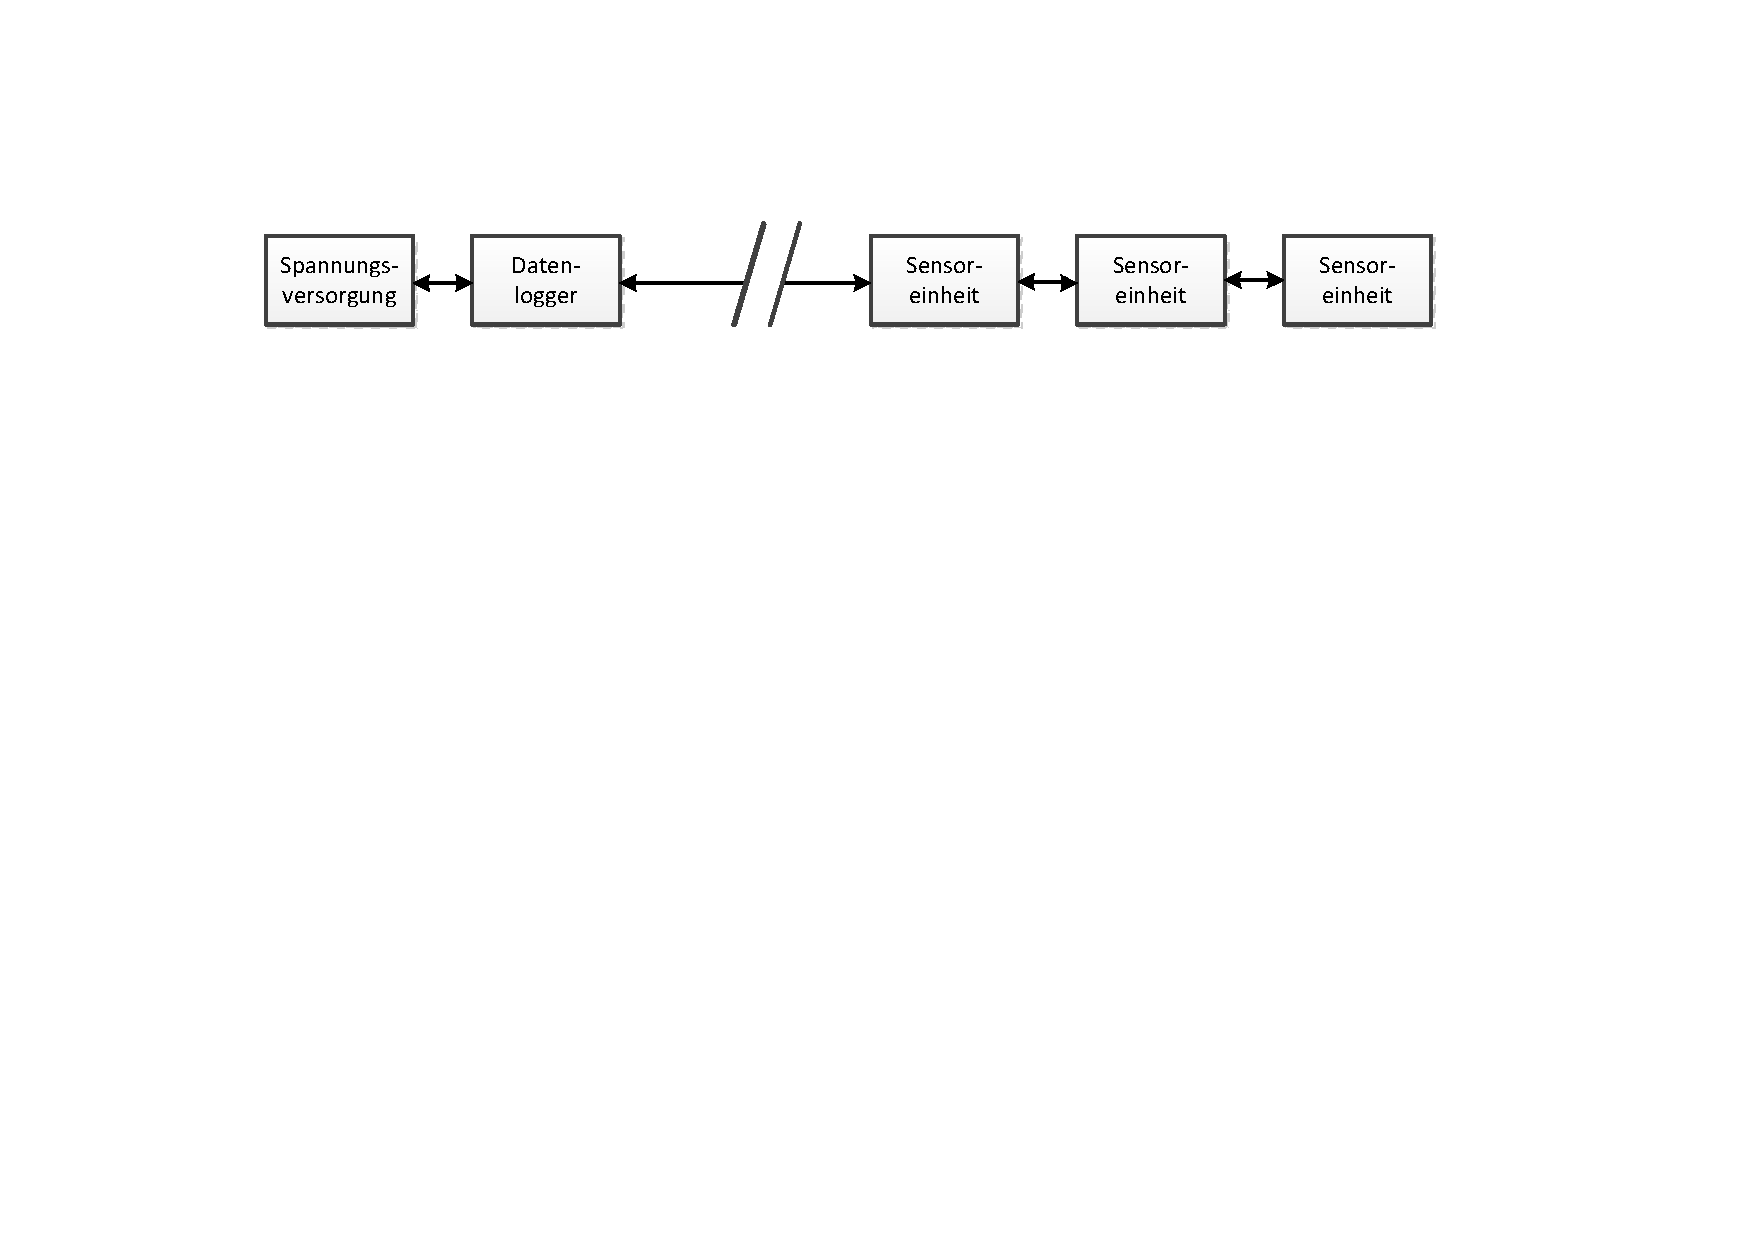
\includegraphics[width=0.8\textwidth]{images/visio/schemaMessanlage.pdf}
	\caption{Schematischer Aufbau einer Messanlage.}
	\label{fig.schemamessanlage}
\end{figure}

Stromversorgung, Verdrahtung, Can-Bus, Terminator, R2D2, C3PO

Die \glspl{sensoreinh} sind in einem wasserdichten Gehäuse verbaut und über wasserdichte Steckverbinder (IP68) untereinander verbunden. 










\section{Datenlogger}\label{sec.manuallogger}
Das Herzstück der Anlage ist der \gls{logger}, der die Kontrolle über die Kommunikation hat, die Messdaten speichert und den Anschluss eines \gls{compi}s für die Konfiguration der Anlage ermöglicht. Im Datenlogger arbeitet ein \emph{ARM Cortex-M4} Prozessor mit 120~MHz Taktgeschwindigkeit. Dieser Prozessor steuert die Kommunikation und wandelt die Messdaten für die Speicherung in lesbare Information um.

\subsection{Anschlüsse}
Der \gls{logger} verfügt über vier Anschlüsse. Abbildung \ref{foto.logger} zeigt einen geöffneten \gls{logger}.

\todo{foto des datenloggers einfügen}
\begin{figure}
	\centering
		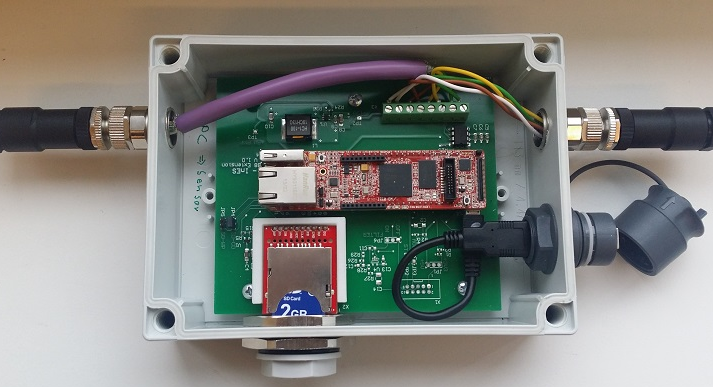
\includegraphics[width=0.8\textwidth]{images/fotos/datenlogger.png}
	\caption{Der Datenlogger in geöffnetem Zustand.}
	\label{foto.logger}
\end{figure}


\subsubsection{Stromversorgung}
Ein Anschluss ist für die Stromversorgung, in Abbildung \ref{foto.logger} auf der rechten Seite. Hier werden \ensuremath{12 V} Gleichspannung angeschlossen. Der Stromverbrauch ist abhängig von der Anzahl angeschlossener Sensoren.


\subsubsection{Busanschluss}
Über den zweiten Anschluss wird das Kabel des \gls{bussys}s angeschlossen, in Abbildung \ref{foto.logger} auf der linken Seite unten. Der Steckverbinder ist wasserdicht (IP68, Binder), damit kein Regen- oder Kondenswasser in den \gls{logger} eindringen kann. Die Messstation verwendet CAN-Bus für die Kommunikation, da dieser Standard ein sehr robustes Protokoll für die Sicherstellung der korrekten und fehlerfreien Übertragung hat. 

\subsubsection{Schnittstelle zum Computer}
Ein wasserdichter Steckverbinder (in Abbildung \ref{foto.logger} auf der linken Seite oben) für ein \gls{usb}-Kabel erlaubt den Anschluss eines Computers oder auch einen Smartphones. Über eine serielle Schnittstelle kann dann die Messstation konfiguriert werden. Der Anschluss eines \gls{compi}s und die Konfiguration ist in den Abschnitten \ref{ssec.manualserial} bis \ref{ssec.befehle} ab Seite \pageref{ssec.manualserial} im Detail beschrieben.

\subsubsection{Speicherkarte}
Die Speicherkarte kann über einen wasserdichten Schraubdeckel (Abbildung \ref{foto.logger}: oben) ausgewechselt werden, ohne dass das ganze Gehäuse des \gls{logger}s geöffnet werden muss. Der Umgang mit der Speicherkarte ist im Abschnitt \ref{sssec.sdformat} ab Seite \pageref{sssec.sdformat} erklärt.











\section{Sensor}\label{sec.manualsensor}
Die \gls{sensoreinh} der Anlage verfügen über einen Beschleunigungssensor, einen Mikroprozessor und zwei Anschlüsse für das Bussystem (Abbildung \ref{foto.sensoreinh}). Der Sensor misst über die Beschleunigung die Vibrationen, die vom Einschlag des Geschiebes verursacht werden. Der Mikroprozessor wertet die Messdaten aus und erkennt nach vorher definierten Kriterien die Ereignisse, deren Daten gesammelt werden sollen. Diese bereinigten Daten werden dann über das \gls{bussys} an den \gls{logger} übertragen.

\todo{foto des datenloggers einfügen}
\begin{figure}
	\centering
		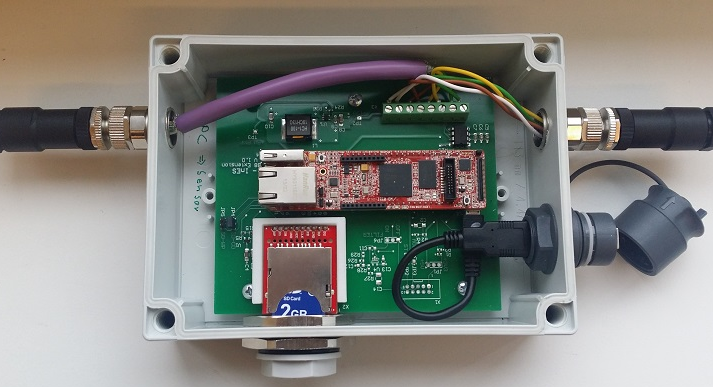
\includegraphics[width=0.8\textwidth]{images/fotos/datenlogger.png}
	\caption{Die Sensoreinheit in geöffnetem Zustand.}
	\label{foto.logger}
\end{figure}

\subsection{Beschleunigungssensor}
Der Beschleunigungssensor (\emph{Analog Devices ADXL001-70}) misst Beschleunigungen zwischen -70~g und +70~g. Ein g entspricht der Beschleunigung durch die Erdanziehungskraft, ungefähr 10~\ensuremath{m/s^2}. Sollten die Vibrationen stärkere Beschleunigungen erzeugen, kann entweder die Konstruktion der Messanlage angepasst werden um die Vibrationen abzuschwächen oder der Sensor wird ausgewechselt. Aus der Baureihe \emph{ADXL001} von \emph{Analog Devices} sind auch Sensoren mit Messbereichen von \ensuremath{\pm}250 g und \ensuremath{\pm}500 g erhältlich. Diese Modelle geben Messsignale im gleichen Spannungsbereich aus wie das verwendete Modell ADXL001-70 und können daher ohne Umkonfiguration oder Anpassungen an der \gls{software} verwendet werden.
Der Sensor muss mit einem Objekt in festem Kontakt stehen, auf dem die Geschiebekörner aufschlagen. Dazu muss entweder das Gehäuse mit einer Platte verbunden werden, oder das Sensorkabel wasserdicht aus dem Gehäuse zu einer Platte geführt werden.

\subsection{A/D-Wandler}
Die Messsignale vom Beschleunigungssensor werden von einem 12-Bit-\gls{adwandler} digitalisiert. Der \gls{adwandler} kann theoretisch mit bis zu 200000~Hz betrieben werden.


\subsection{Mikroprozessor}
Der \emph{ARM Cortex-M4} mit 120~MHz Taktfrequenz hat weit mehr Rechenleistung, als für die vorliegende Anwendung benötigt wird. Sollten komplexere Algorithmen für die Erkennung von Ereignissen, für die Filterung der Messdaten oder für die Verarbeitung der Signale benötigt werden, wäre dies dank der bereits vorhandenen Rechenleistung möglich.

\subsection{Anschlüsse}
Die \gls{sensoreinh} hat zwei Anschlüsse für das Bussystem. Mit dieser Bauweise ist es möglich, die \gls{stichleitung} zum \gls{transceiver} möglichst kurz zu halten, um die Signalqualität möglichst wenig negativ zu beeinflussen. Die Anschlüsse sind wasserdicht (IP68).














\section{Bussystem}\label{sec.manualbus}
Als Bussystem wird CAN-Bus verwendet. Mit einer Datenübertragungsrate von 1~MBit/s bis zu einer Kabelgesamtlänge von 40~m, resp 125~kBit/s bis zu 500~m eignet sich CAN-Bus für diese Messstation sehr gut. Es sind keine Kabellängen zu erwarten, die weit über 40~m hinausgehen. CAN-Bus ist des Weiteren sehr robust gegenüber Umwelteinflüssen, die die Übertragung stören könnten.

\subsection{Kabel}
Die Kabel der Messstation verfügen über 4 Leitungen, die jeweils paarweise verdrillt sind. Zusätzlich zu den Leitungen ist eine Zugentlastung zum Schutz vor mechanischer Beschädigung im Kabel enthalten. Um die zwei Aderpaare und die Zugentlastung ist ein metallisches Geflecht als Schild angebracht, das sowohl gegen mechanische Beschädigung als auch gegen elektrische Störeinflüsse schützt. Die PVC-Hülle des Kabels ist noch ein zusätzlicher mechanischer Schutz. 

Ein Aderpaar wird für die Spannungsversorgung verwendet, das zweite Aderpaar für die Kommunikation auf dem Bussystem.

\subsection{Abschlusswiderstände}
Damit die Bus-Signale an den Enden der Leitung nicht reflektiert werden und die Übertragung stören, müssen an beiden Enden des Bussystems Abschlusswiderstände eingesetzt werden.  Die Abschlusswiderstände (120 \ensuremath{\ohm}) verbinden die Anschlüsse CANH und CANL auf der Leiterplatte und werden wie in Abbildung \ref{fig.terminator} angebracht.

\begin{figure}
	\centering
		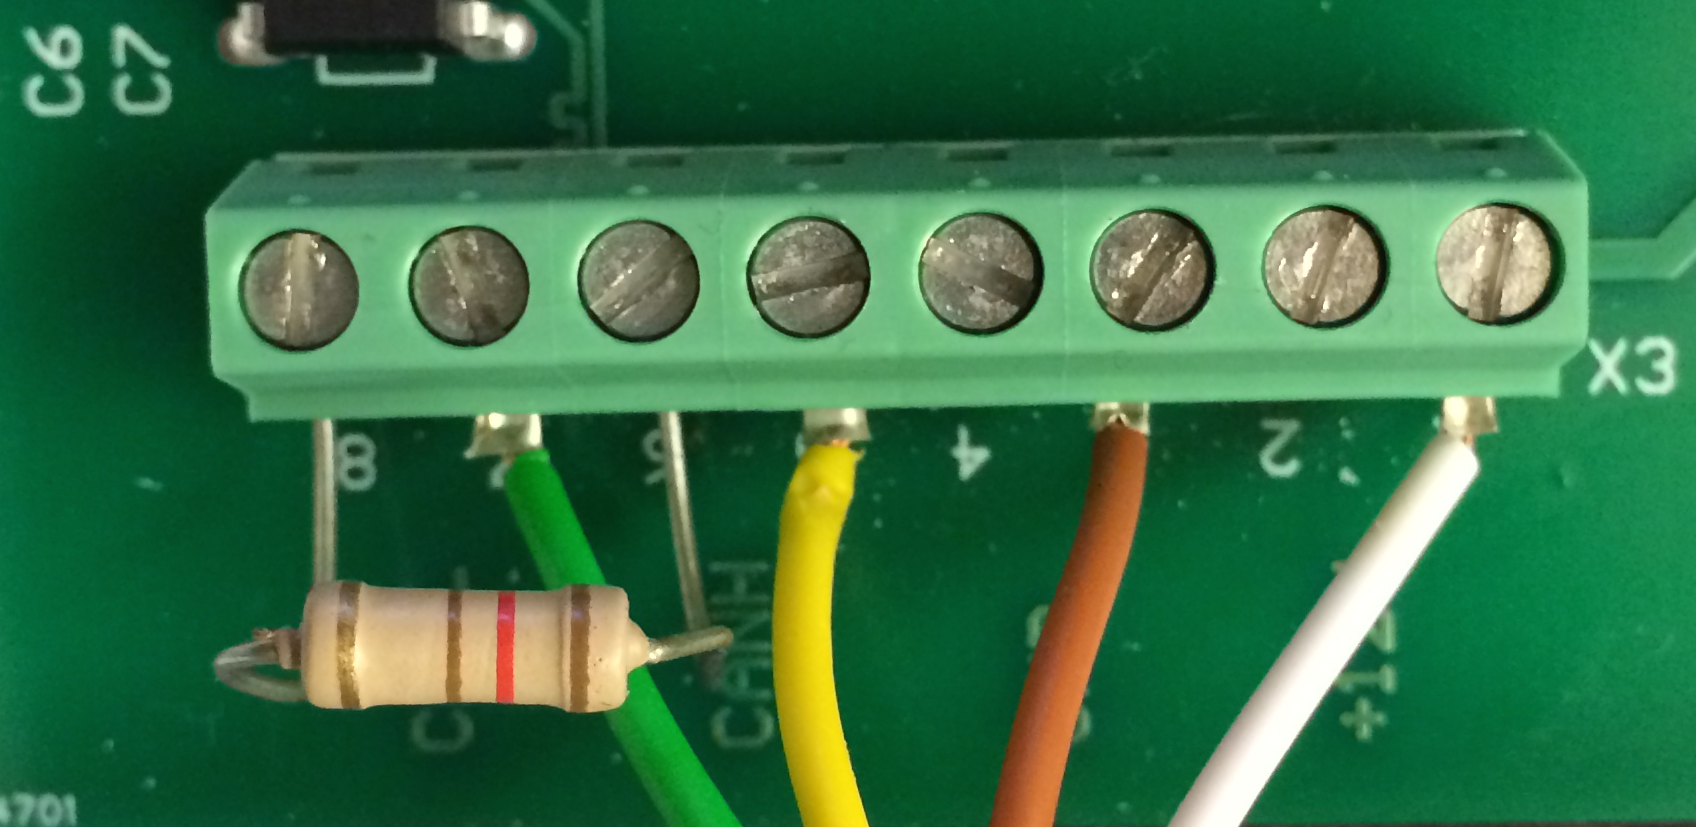
\includegraphics[width=0.8\textwidth]{images/fotos/terminator.png}
	\caption{Anbringung des \gls{terminator}s.}
	\label{fig.terminator}
\end{figure}

\subsection{Steckverbinder}
Die Steckverbinder sind fünfpolig und wasserdicht (IP68). Die Pole sind gemäss Tabelle \ref{table.stecker} bestückt, die Polnummerierung in Stecker und Buchse sind in den Abbildungen \ref{fig.polbuchse} und \ref{fig.polstecker} dargestellt.

\begin{table}
\begin{tabular}{|l|l|l|l|}
\hline \textbf{Pol Nr.}      & \textbf{Leitung} & Anschluss Schraubklemme & Aderfarbe\\ 
\hline 1 & Spannungsversorgung +12~V & +12V & weiss \\
\hline 2 & Spannungsversorgung 0~V & GND & braun \\
\hline 3 & unbenutzt &  &  \\
\hline 4 & CAN-Bus High & CANH & gelb \\
\hline 5 & CAN-Bus Low & CANL & grün \\
\hline 
\end{tabular}
\caption{Steckerbestückung des \gls{bussys}s.}
\label{table.stecker}
\end{table}  

\begin{figure}
\centering
\begin{minipage}{0.5\textwidth}
\centering
		
\includegraphics[width=0.8\textwidth]{images/Polbelegung_Buchse.pdf}
	\captionof{figure}{Polnummerierung in der Buchse.}
	\label{fig.polbuchse}
\end{minipage}%
\begin{minipage}{0.5\textwidth}
\centering
		
\includegraphics[width=0.8\textwidth]{images/Polbelegung_Stecker.pdf}
	\captionof{figure}{Polnummerierung im Stecker.}
	\label{fig.polstecker}
\end{minipage}
\end{figure}

Auf der Leiterplatte der \gls{sensoreinh} ist eine Schraubklemmenleiste mit 8 Anschlüssen angebracht. Hier werden die von den Buchsen kommenden Leitungen angeschlossen. Jeweils zwei benachbarte Anschlüsse sind zusammengeschaltet, damit jede Leitung einzeln fest verschraubt werden kann (Abbildung \ref{fig.kabel}). Es wird nicht empfohlen, zwei gleiche Leitungen in einer einzelnen Schraubklemme zusammen zu verschrauben.

\begin{figure}
	\centering
		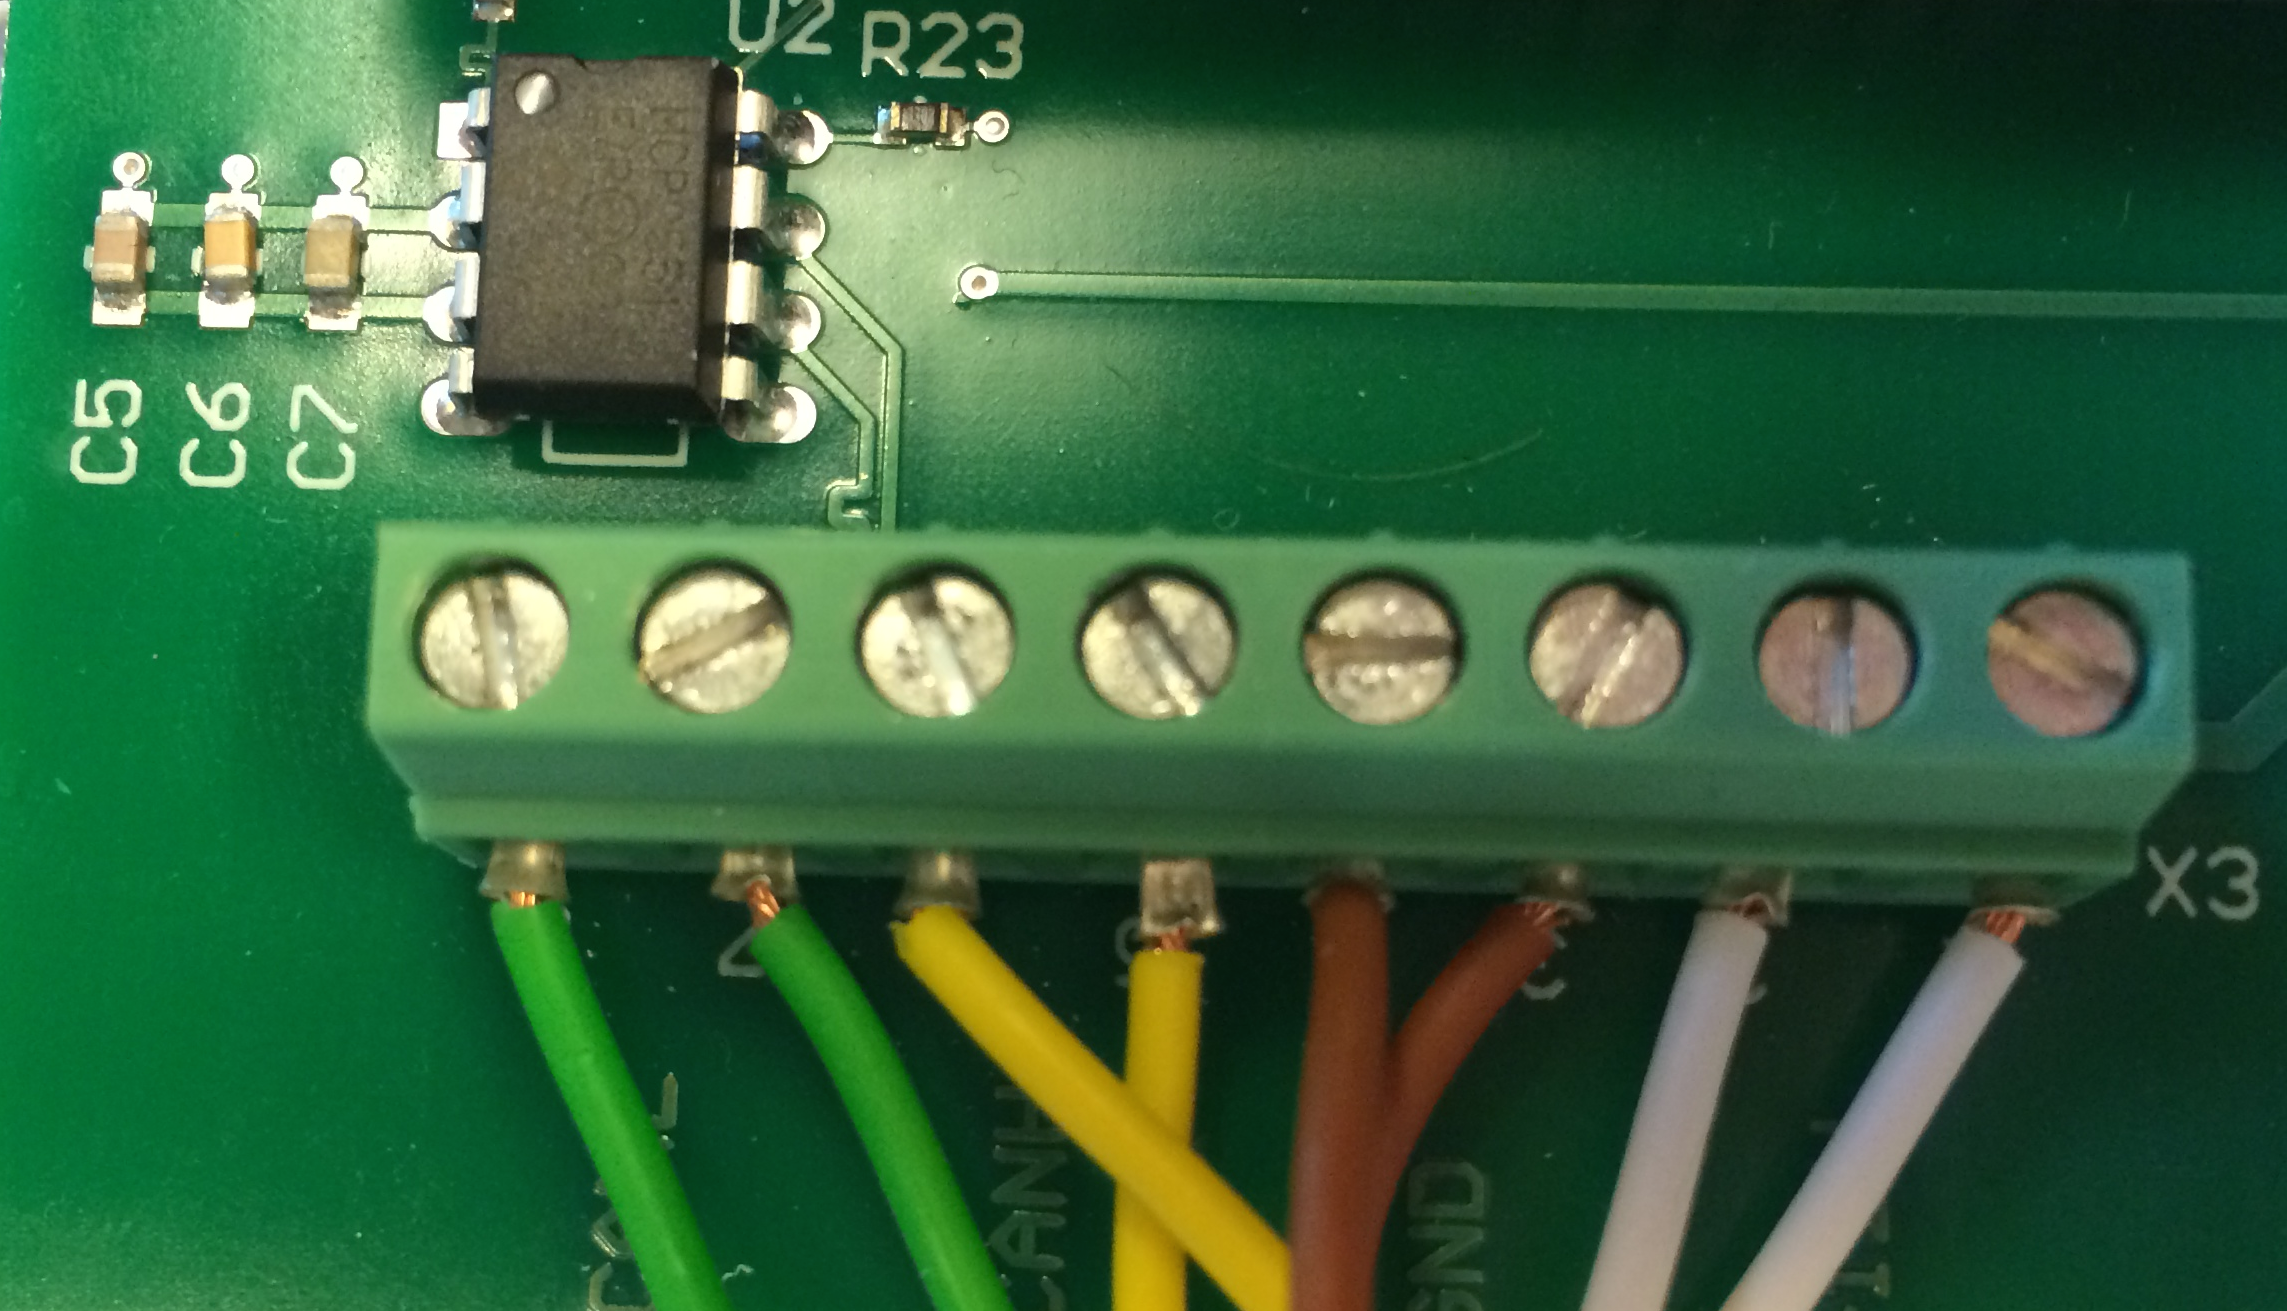
\includegraphics[width=0.8\textwidth]{images/AnschlussKabel.png}
	\caption{Anschluss der Leitungen an den Schraubklemmen.}
	\label{fig.kabel}
\end{figure}









\section{Ereignis}\label{sec.manualimpact}
Als Ereignis wird eine Signalform bezeichnet, die einem Einschlag eines Steins auf dem Sensor entspricht. Um Ereignisse zu erkennen, wird ein \gls{threshold} für den Signalpegel definiert. Wird dieser Wert überschritten, beginnt ein Ereignis. Sobald der Signalpegel für eine gewisse Zeit unterhalb des \gls{threshold}s geblieben ist, ist das Ereignis beendet. Das Verfahren der Ereigniserkennung wird im Abschnitt \ref{subsec.sw_ereignis} ab Seite \pageref{subsec.sw_ereignis} im Detail erklärt.

Ein Beispiel eines Ereignisses ist in Abbildung \ref{fig.impactraw} gegeben. Es handelt sich um den Einschlag eines Golfballs auf einer Aluminiumplatte, unter der der Beschleunigungssensor montiert ist. Die schwarz gestrichelten Geraden zeigen den \gls{threshold}, die roten Geraden zeigen den erkannten Anfang und Ende des \gls{ereignis}ses. Das Ende des \gls{ereignis}ses wird von der \gls{ereignisdet} auf jenen Messpunkt gelegt, an dem der Signalpegel den \gls{threshold} vor dem \gls{timeout} das letzte Mal unterschritten hat. Die Messwerte vor der dem \gls{timeout} werden je nach Detail-Level abgeschnitten. Die folgende Beschreibung der Detail-Level bezieht sich auf dieses Beispiel-Ereignis.

\begin{figure}
	\centering
		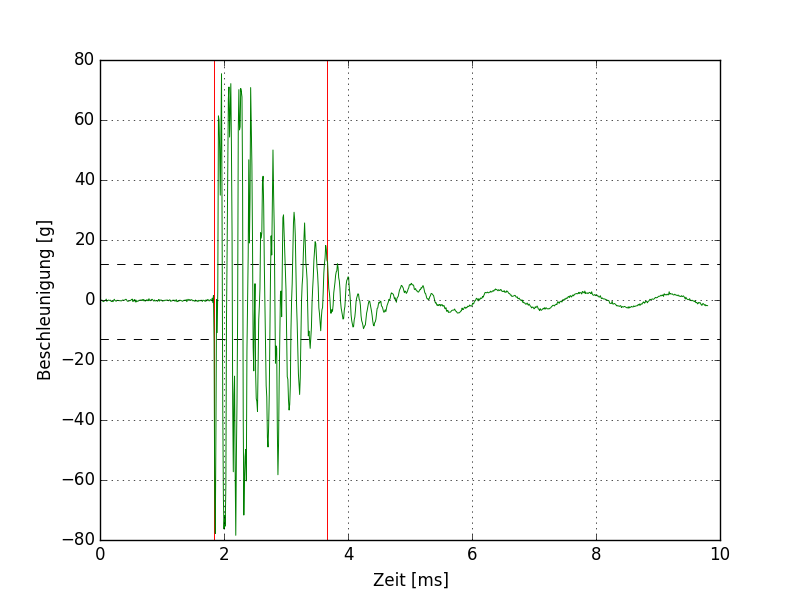
\includegraphics[width=0.8\textwidth]{images/raw.png}
	\caption{Beispiel von Rohdaten.}
	\label{fig.impactraw}
\end{figure}

\subsection{Detail-Level}\label{ssec.detaillevel}
Die Messstation kann Daten mit unterschiedlichen Detailgraden speichern. Jede \gls{sensoreinh} kann individuell auf einen Detail-Level konfiguriert werden.

\begin{itemize}
\item raw
\item detailed
\item peaks only
\item sparse
\item off
\end{itemize}


\subsubsection{Rohdaten (raw)}
Im Modus 'raw' werden Rohdaten ohne Ereigniserkennung übertragen und gespeichert. Es resultiert eine lückenlose Erfassung aller Messpunkte. Abbildung \ref{fig.detailraw} zeigt in Grün, welche Daten des Beispielereignisses im Modus 'raw' übertragen werden.


\begin{figure}
	\centering
		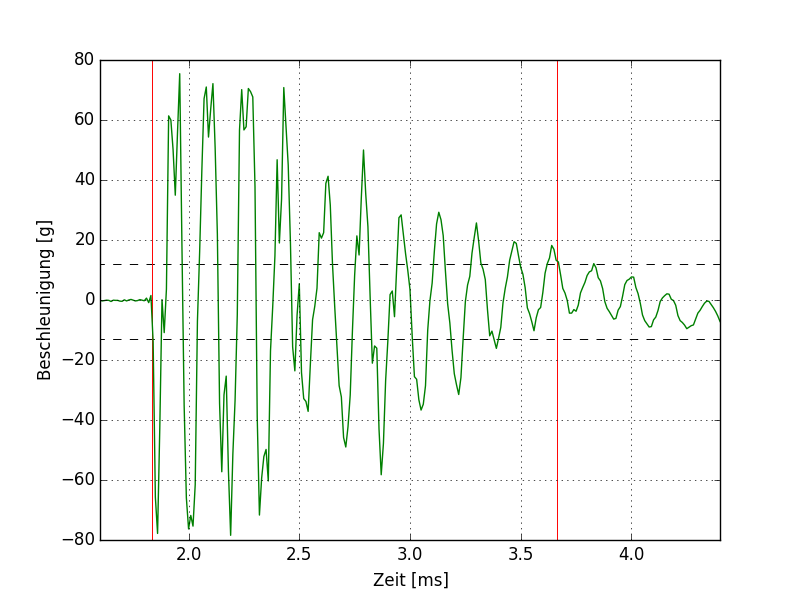
\includegraphics[width=0.8\textwidth]{images/rawshort.png}
	\caption{Detail-Level 'raw'.}
	\label{fig.detailraw}
\end{figure}

\paragraph{Datenaufkommen} Das Datenaufkommen ist in diesem Modus am grössten. Für jedes \gls{sample} wird ein 8-bit Wert abgespeichert. Bei einer \gls{fs} von 10000~Hz fallen also 10000~Byte Daten pro Sensor und Sekunde an.

\paragraph{Beispieldaten} In der Datei wird beim Start der Aufzeichnung eingetragen, wann die Aufzeichnung (in Sekunden seit 0:00 Uhr, 1.1.1970) beginnt und wie viele Samples gemessen werden sollen. Danach folgen nur noch Datenwerte zwischen -128 und 127. Listing \ref{list.sampleraw} zeigt den Anfang und Ende eines Eintrags aus dem Rohdatenmodus. Die Messwerte sind durch Kommas getrennt, ein Strichpunkt markiert das Ende des Eintrags.

\begin{lstlisting}[caption=Beispieldaten auf Detail-Level 'raw', label=list.sampleraw]
start=1417865674,samples=600000;0,3,15,-12,15, ... 97,12,-45,-100;
\end{lstlisting}


\subsubsection{Detaillierte Ereignisdaten (detailed)}
Die \gls{ereignisdet} sucht den Beginn und das Ende des Ereignisses. Es werden sämtliche \glspl{sample} des Ereignisses übertragen. Im Konfigurationsmenü wird dieser Modus als 'detailed' bezeichnet. In Abbildung \ref{fig.detaildetailed} entspricht die grüne Kurve den gespeicherten Daten.

\begin{figure}
	\centering
		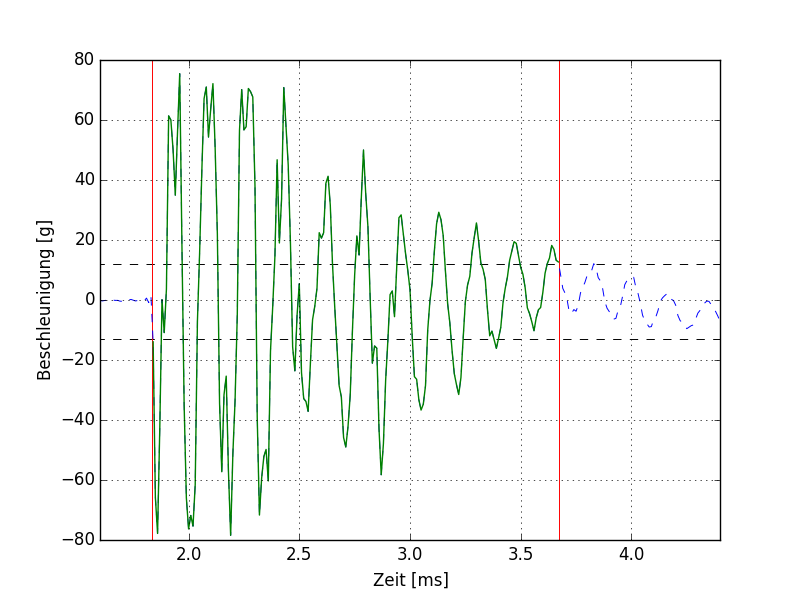
\includegraphics[width=0.8\textwidth]{images/detailed.png}
	\caption{Detail-Level 'detailed'.}
	\label{fig.detaildetailed}
\end{figure}

\paragraph{Datenaufkommen} Pro \gls{sample} wird ein Byte abgespeichert, der Startzeitpunkt und die Dauer belegen zusammen sechs Byte pro Ereignis. Die Datenmenge variiert mit der Dauer der Ereignisse. Es wird geschätzt, dass bei hohem Ereignisaufkommen während etwa 10~\% der Messzeit ein Ereignis vorliegt. Somit wird die Datenrate ungefähr ein Zehntel der \gls{fs} in Byte/Sekunde sein.

\paragraph{Beispieldaten} Das Format der Datenablage ist im Detail-Level 'detailed' genau gleich wie bei 'raw'. Der Eintrag enthält jedoch nur Messwerte von einem einzigen Ereignis und ist daher viel kürzer (Listing \ref{list.sampledetailed}).

\begin{lstlisting}[caption=Beispieldaten auf Detail-Level 'detailed', label=list.sampledetailed]
start=1417865674,samples=187;-125,-107,-12,15, ... 43,7,-45;
\end{lstlisting}


\subsubsection{Peaks (peaks only)}
Die Ereigniserkennung sucht im Modus 'peaks only' den Beginn und das Ende und somit die Dauer des Ereignisses. Ausserdem werden alle Peakspitzen mit dem \gls{timestamp} und Höhe des Ausschlags gespeichert.
\begin{figure}
	\centering
		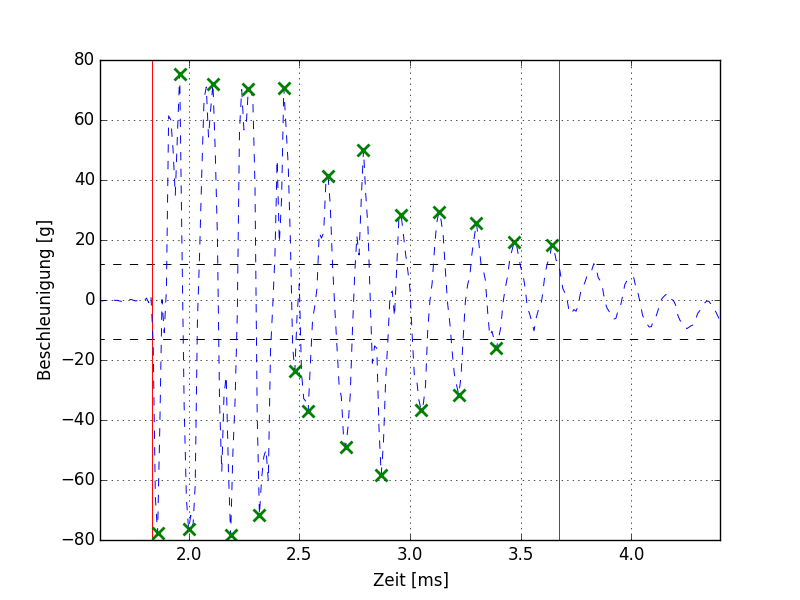
\includegraphics[width=0.8\textwidth]{images/peaks.png}
	\caption{Detail-Level 'peaks'.}
	\label{fig.detailpeaks}
\end{figure}

\paragraph{Datenaufkommen} Für die Eckdaten (Beginn, Dauer, Anzahl Peaks, maximaler Ausschlag) fallen 8 Byte Daten an. Jeder Peak benötigt zwei Byte: ein Byte für die Anzahl Samples seit dem letzten Peak und ein Byte für die Höhe des Ausschlags. In der Abbildung \ref{fig.detailsparse} zeigt die blau gestrichelte Linie den Verlauf der Messkurve, die roten Geraden markieren Beginn und Ende des \gls{ereignis}ses. Die grünen 'X' markieren die Peakspitzen, die übertragen werden.

\paragraph{Beispieldaten} Der Eintrag enthält die Startzeit in Sekunden, die Dauer in Samples und die Anzahl Peaks. Danach folgen Wertepaare mit dem Abstand zum vorherigen Peak (resp. zum Beginn des Ereignisses) in Samples und der Peakhöhe (Listing \ref{list.samplepeaks}). Der Maximalwert des Ereignisses entspricht dem höchsten Peak und wird deshalb nicht extra gespeichert.

\begin{lstlisting}[caption=Beispieldaten auf Detail-Level 'peaks only', label=list.samplepeaks]
start=1417865674,samples=187,nrpeaks=22;3 -120,12 110, ..., 18 68,7 -55;
\end{lstlisting}

\subsubsection{Minimale Daten (sparse)}
Im Modus 'sparse' werden nur Eckdaten des \gls{ereignis}ses gespeichert: Beginn und Dauer, Anzahl Peaks und maximaler Ausschlag. Dafür genügen acht Byte pro Ereignis. Die Eckdaten sind in Abbildung \ref{fig.detailsparse} dargestellt.

\begin{figure}
	\centering
		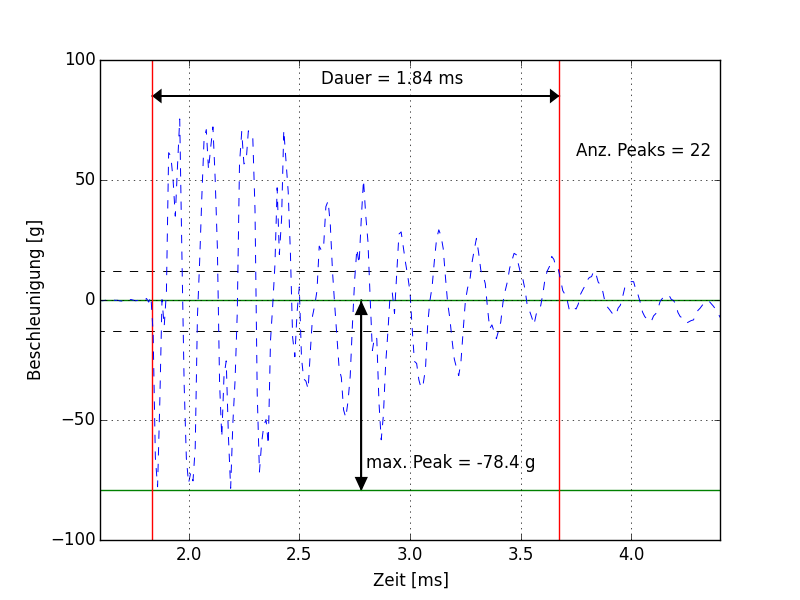
\includegraphics[width=0.8\textwidth]{images/sparse.png}
	\caption{Detail-Level 'sparse'.}
	\label{fig.detailsparse}
\end{figure}

\paragraph{Datenaufkommen} Der \gls{timestamp} für den Beginn des \gls{ereignis}ses benötigt vier Byte, die Dauer (Anzahl Samples) zwei Byte. Die Anzahl Peaks und der maximale Ausschlag belegen je ein Byte.

\paragraph{Beispieldaten} Der Eintrag enthält die Startzeit in Sekunden, die Dauer in Samples, die Anzahl Peaks und den maximalen Ausschlag (Listing \ref{list.samplesparse}). 
\begin{lstlisting}[caption=Beispieldaten auf Detail-Level 'sparse', label=list.samplesparse]
start=1417865674,samples=187,nrpeaks=22,max=-125;
\end{lstlisting}

\subsubsection{Inaktiv (off)}
Die \gls{sensoreinh} kann in den Detail-Level 'off' gesetzt werden. In diesem Fall startet sie auch keine Messung, wenn der \gls{logger} alle \glspl{sensoreinh} startet.

In diesem Detail-Level fallen keine Daten an.


\section{Konfiguration}\label{sec.manualkonfig}


\subsection{Anschluss eines Computers}\label{ssec.manualserial}
Am \gls{usb}-Anschluss des \gls{logger}s kann ein \gls{compi} angeschlossen werden, um auf die serielle Schnittstelle des \gls{logger}s zuzugreifen. Um die serielle Schnittstelle zu verwenden, wird ein \gls{terminalemu} wie \emph{PuTTY} oder \emph{minicom} benötigt. um mit \emph{PuTTY} eine Verbindung aufzubauen, muss die Schnittstelle und die Übertragungsrate (Baud) angegeben werden. Die Übertragungsrate ist 9600 baud, die Schnittstelle kann variieren. 

\paragraph{Windows} Unter \emph{Windows} erfolgt die Verbindung auf eine der COMx-Schnittstellen. Die Nummer der COM-Schnittstelle kann im Geräte-Manager herausgesucht werden, die Bezeichnung lautet 'mbed Serial Port (COMx)', wobei 'x' eine Nummer ist. In PuTTY muss nur 'COMx' angegeben werden.

\paragraph{Linux} Unter \emph{Linux} findet man die Schnittstellenbezeichnung mit dem Befehl 'ls /dev/ttyACM*' heraus, in \emph{PuTTY} wird dann '/dev/ttyACMx' angegeben. 

\paragraph{Mac OS X} Unter \emph{Mac OS X} lautet der Befehl 'ls /dev/tty.usbmodem*', der in einem Terminal eingegeben werden muss. Als \gls{terminalemu} kann 'screen' verwendet werden. Auf Apple Mac Computern mit \gls{usb} 3.0 kann es zu Schwierigkeiten mit der Verbindung kommen. Den Herstellern des Prozessorboards ist dies bekannt, sie arbeiten an einer Lösung.

Die Einstellungen für die serielle Schnittstelle sind normalerweise bereits korrekt gesetzt. Es werden 8 Datenbits verwendet, 1 Stopbit und keine Parität (parity).

Weitere Hilfe für die Verwendung eines \gls{terminalemu}s findet man unter \url{http://developer.mbed.org/handbook/Terminals}.



\subsection{Menü}\label{ssec.menu}
Beim Herstellen der Verbindung über einen \gls{terminalemu} wird das Basis-Menü angezeigt. Durch Eingabe der Zahl wird der entsprechende Menü-Eintrag gewählt. Im Folgenden wird das gesamte Menü im Detail beschrieben.

Das Basis-Menü (siehe Listing \ref{list.basemenu}) listet alle Überwachungs- und Konfigurations-Möglichkeiten auf. 

\begin{lstlisting}[caption=, label=list.basemenu]
 1) list files
 2) format SD card
 3) mount SD card
 4) unmount SD card
 5) logger status
 6) start/stop logging
 7) sensor parameters
 8) sensor states
 9) reset timestamp
10) internal clock
11) config file
\end{lstlisting}

\paragraph{Dateien auflisten} Mit dem Befehl 'list files' wird eine Liste aller Dateien auf der SD-Karte angezeigt. Die Liste enthält die Dateigrösse sowie den Dateinamen, siehe Abschnitt \ref{sssec.listfiles}.

\paragraph{SD-Karte formatieren} Um die SD-Karte für den ersten Gebrauch vorzubereiten, sollte sie formatiert werden. Dies erfolgt von Vorteil auf einem \gls{compi}, kann aber auch im \gls{logger} mit dem Befehl 'format SD card' gemacht werden, siehe Abschnitt \ref{sssec.sdformat}.

\paragraph{SD-Karte anmelden} Nach dem Einsetzen einer SD-Karte erkennt der \gls{logger} dies normalerweise automatisch. Es kann jedoch vorkommen, dass der \gls{logger} auf die neue Karte aufmerksam gemacht werden muss. Dies erfolgt mit dem Befehl 'mount SD card', siehe Abschnitt \ref{sssec.sdmount}.

\paragraph{SD-Karte abmelden} Vor dem Entfernen der SD-Karte müssen alle Dateien geschlossen werden. Dies erfolgt mit dem Befehl 'unmount SD card', siehe Abschnitt \ref{sssec.sdunmount}.

\paragraph{Status des Datenloggers} Mit dem Befehl 'logger status' werden einige Betriebszustandsdaten des Datenloggers angezeigt, siehe Abschnitt \ref{sssec.loggerstate}.

\paragraph{Aufzeichnung starten/stoppen} Um die Aufzeichnung im ganzen System zu starten oder zu stoppen wird der Befehl 'start/stop logging' verwendet, siehe Abschnitt \ref{sssec.startstop}.

\paragraph{Sensor-Einstellungen} Mit dem Befehl 'sensor parameters' kann eine einzelne \gls{sensoreinh} oder alle \glspl{sensoreinh} zusammen konfiguriert werden. Siehe Abschnitt \ref{sssec.sensorparam}.

\paragraph{Status der Sensoreinheiten} Der Betriebszustand aller angeschlossenen \glspl{sensoreinh} kann mit dem Befehl 'sensor state' (siehe \ref{sssec.sensorstate}) aufgelistet werden.

\paragraph{Timestamp zurücksetzen} Um den Timestamp in allen \glspl{sensoreinh} auf Null zurückzustellen, wird der Befehl 'reset timestamp' verwendet. Siehe Abschnitt \ref{sssec.timestamp}.

\paragraph{Interne Uhr} Die interne Uhr wird mit den Befehl 'internal clock' eingestellt, Abschnitt \ref{sssec.intclock} beschreibt dies im Detail.

\paragraph{Konfigurations-Datei} Mit dem Befehl 'config file' wird die Konfiguration der Sensoren abgespeichert oder aus einer Datei eingelesen, siehe Abschnitt \ref{sssec.configfile}.

\subsection{Befehle}\label{ssec.befehle}

\subsubsection{Dateiliste}\label{sssec.listfiles}
\begin{lstlisting}[caption=, label=list.]
f:       90 /mci/config.txt
f:   122086 /mci/s02_1214_0530.dat

 0) exit
\end{lstlisting}


\subsubsection{SD-Karte formatieren}\label{sssec.sdformat}
\begin{lstlisting}[caption=Untermenü SD-Karte formatieren, label=list.sdformat]
 1) confirm formatting of SD card.
    All data will be erased.
 0) cancel
\end{lstlisting}

Beim Formattieren werden alle Dateien auf der SD-Karte gelöscht, inklusive der Konfigurationsdatei mit allen Sensor-Einstellungen. Der Befehl 'format SD card' holt vor der Ausführung nochmals eine Bestätigung ein, ob sich der Benutzer wirklich sicher ist, dass er alle Dateien löschen will (Listing \ref{list.sdformat}). Während dem Formatieren wird die Meldung \ref{list.sdformatting} angezeigt.

\begin{lstlisting}[caption=Statusmeldung SD formatieren, label=list.sdformatting]
formatting SD Card
\end{lstlisting}

Sind beim Formatieren Fehler aufgetreten, erhält man die Fehlermeldung \ref{list.sdformatfail}. In diesem Fall sollte die Karte in einem \gls{compi} geprüft und formatiert werden.

\begin{lstlisting}[caption=Fehlermeldung SD formatieren, label=list.sdformatfail]
Formatting SD card FAILED. Please use a Computer to format the card.
\end{lstlisting}

Bei erfolgreicher Formatierung wird die Meldung \ref{list.sdformatsuccess} ausgegeben. 

\begin{lstlisting}[caption=Erfolgsmeldung SD formatieren, label=list.sdformatsuccess]
Formatting done
Returning to base menu.
\end{lstlisting}


\subsubsection{SD-Karte anmelden}\label{sssec.sdmount}
Damit Dateien auf die SD-Karte geschrieben werden können, muss sie vorher erkannt werden. Normalerweise geschieht dies, sobald die Karte eingesetzt wird. Wenn keine SD-Karte erkannt wird, wird dies im Basismenü angezeigt wie im Listing \ref{list.sdmountfail}. Durch den Aufruf des Befehls 'mount SD card' im Basismenü (Listing \ref{list.basemenu}) kann die eingesetzte SD-Karte angemeldet werden.

Nach erfolgreicher Anmeldung der SD-Karte wird das Basismenü angezeigt. 

Wenn keine SD-Karte erkannt werden kann, wird eine Fehlermeldung \ref{list.sdmountfail} ausgegeben.

\begin{lstlisting}[caption=Fehlermeldung SD-Karte anmelden, label=list.sdmountfail]
No SD card detected! Please insert card and try again!
\end{lstlisting}


\subsubsection{SD-Karte abmelden}\label{sssec.sdunmount}
Bevor die SD-Karte aus dem \gls{logger} entfernt wird, sollte sie abgemeldet werden. Der \gls{logger} schliesst bei diesem Vorgang alle geöffneten Dateien, um Datenverlust zu vermeiden. Da beim Abmelden der Karte die Aufzeichnung der Daten gestoppt wird, wird vorher eine Bestätigung verlangt (Listing \ref{list.sdunmount}).

\begin{lstlisting}[caption=Untermenü SD-Karte abmelden, label=list.sdunmount]
 1) unmount SD card
    This will stop logging and close all data files.
 0) cancel
\end{lstlisting}

Falls die Konfiguration der Sensoren verändert, aber noch nicht in die Konfigurationsdatei geschrieben wurde, wird eine Warnung angezeigt (Listing \ref{list.sdunmountwarn}). Die Konfiguration bleibt im Speicher des \gls{logger}s erhalten, so lange die Spannungsversorgung angeschlossen ist und kann auch auf der neuen SD-Karte gespeichert werden.

\begin{lstlisting}[caption=Warnung vor SD-Karte abmelden bei ungespeicherter Konfiguration, label=list.sdunmountwarn]
******************************************************************
* WARNING: sensor configuration data has not been saved to file! *
* If you want to save config to file, cancel now.                *
******************************************************************
\end{lstlisting}

\subsubsection{Logger-Status}\label{sssec.loggerstate}
Mit dem Befehl 'logger status' können einige Information über den \gls{logger} angezeigt werden.

\begin{lstlisting}[caption=Untermenü Logger-Status, label=list.loggerstatus]
Time: Sat Dec 6 18:00:00 2014
Started?: 1
\end{lstlisting}


\subsubsection{Starten und stoppen der Aufzeichnung}\label{sssec.startstop}
Um die Datenspeicherung im \gls{logger} zu unterbrechen oder wieder zu starten wird der Befehl 'start/stop logger' verwendet. Beim Aufruf des Befehls wird ein Untermenü gemäss Listing \ref{list.startstop1} oder Listing \ref{list.startstop2} angezeigt.

\begin{lstlisting}[caption=Untermenü Stoppen der Aufzeichnung, label=list.startstop1]
 Logger is running.
 1) stop the logging.
 0) cancel
\end{lstlisting}

Da sich das Menü dem gegenwärtigen Zustand anpasst, sieht es bei gestoppter Aufzeichnung aus wie in Listing \ref{list.startstop2}.

\begin{lstlisting}[caption=Untermenü Starten der Aufzeichnung, label=list.startstop2]
 Logger is stopped.
 1) start the logging.
 0) cancel
\end{lstlisting}

Wenn die Aufzeichnung am Logger gestoppt wird, wird an alle \glspl{sensoreinh} der Befehl zum Aufzeichnungsstopp gesendet. Die Einstellungen zum Detailmodus bleiben in der \gls{sensoreinh} aber erhalten. Beim erneuten Starten der Aufzeichnung im Logger werden auch die \glspl{sensoreinh} wieder gestartet. Es besteht auch die Möglichkeit, einzelne \glspl{sensoreinh} zu stoppen (siehe Abschnitt \ref{sssec.sensorparam}). Eine gestoppte \gls{sensoreinh} bleibt auch beim Starten der Aufzeichnung am \gls{logger} gestoppt, da sie schon vor dem Stopp in diesem Zustand war.

\subsubsection{Sensor-Parameter}\label{sssec.sensorparam}
Die Parameter der Datenerfassung und Ereigniserkennung können für alle \glspl{sensoreinh} gemeinsam oder für jede \gls{sensoreinh} individuell eingestellt werden. Die Auswahl einer einzelnen oder aller \glspl{sensoreinh} erfolgt beim Einstieg in das Untermenü der Sensor-Parameter. Listing \ref{list.sensorsel} zeigt die Auswahl der Sensoren. Die Auswahlliste enthält gleich die aktuellen Werte der Parameter, damit man eine Übersicht hat.


\begin{lstlisting}[caption=Untermenü Sensor-Auswahl, label=list.sensorsel]
 Nr  SID  serial       fs threshold baseline timeout   detail
 1)    2  461bfdf6  10000       200     2047      30      raw
 2)    3  361509a5  10000       150     2000      20    peaks
 ...
 7)    8  1562a010  20000       400     2047      15 detailed
 
 #) Select a sensor from the list.
99) Select all sensors.
 0) cancel
\end{lstlisting}

Nach der Auswahl einer \gls{sensoreinh} gelangt man zur Auswahl des anzupassenden Parameters, Listing \ref{list.sensorparam}. Ist ein einzelner Sensor ausgewählt, werden hier noch einmal die aktuellen Werte der Parameter angezeigt.

\begin{lstlisting}[caption=Untermenü Sensor-Parameter, label=list.sensorparam]
 1) set sampling rate (current: 10000 Hz)
 2) set threshold value (current: 200)
 3) set baseline value (current: 2047)
 4) set timeout (current: 30)
 5) set detail level (current: peaks only)
 6) start or stop recording (current: started)
 0) exit
\end{lstlisting}

\paragraph{Abtastrate} Die Abtastrate legt fest, wie oft pro Sekunde ein Messwert vom Beschleunigungssensor eingelesen werden soll. Die \glspl{sensoreinh} können in einem Bereich zwischen \ensuremath{100 Hz} und \ensuremath{200000 Hz} messen. Die Abtastrate kann in Schritten von \ensuremath{100 Hz} eingestellt werden, Listing \ref{list.paramfs}.

Die Abtastrate hat einen wesentlichen Einfluss auf die zu übertragende und zu speichernde Datenmenge, die benötigte Rechenleistung. Davon wiederum hängt die Zeitspanne ab, wie lange die Messstation ohne Wartung betrieben werden kann. Es wird deshalb empfohlen, die Abtastrate nur so hoch einzustellen, wie es wirklich benötigt wird. Wie hoch dieser Wert ist, hängt stark von den geplanten Auswertungen ab.

\begin{lstlisting}[caption=Untermenü Abtastrate, label=list.paramfs]
 #) Enter sampling rate in Hz. (multiple of 100 Hz in range 100..200'000 Hz)
 0) cancel
\end{lstlisting}

Bei Eingabe einer ungültigen oder nicht unterstützten Abtastrate wird eine Fehlermeldung ähnlich Listing \ref{list.paramfserror} angezeigt.

\begin{lstlisting}[caption=Fehlermeldung bei ungültiger Abtastrate, label=list.paramfserror]
Sampling rate 220000 Hz not supported, too high.
\end{lstlisting}

Bei einer Änderung der Abtastrate wird automatisch der Timestamp zurückgesetzt, damit die Zuweisung der Messdaten zu einem Zeitpunkt weiterhin erfolgen kann.

\paragraph{Ereigniserkennung} Die \gls{ereignisdet} hat drei Parameter, die die Form der gesuchten \glspl{ereignis} bestimmen.  Abbildung \ref{fig.params} illustriert die Zusammenhänge zwischen \gls{threshold} und \gls{nullpegel} sowie die Funktionsweise des \gls{timeout}s.

\paragraph{Threshold} Der \gls{threshold} (Schwellenwert) ist ein Parameter der Ereigniserkennung. Er bestimmt, ab welcher Abweichung vom Nullwert ein Signal als Peak betrachtet werden soll. Bei der Wahl des \gls{threshold}s ist zu beachten, dass der \gls{threshold} auf beide Seiten des Nullwerts gilt. Daher darf die Summe des \gls{nullpegel}s und des \gls{threshold}s nicht den maximalen Wert (4096) des \gls{adwandler}s überschreiten. Ebenso muss der Wert des \gls{threshold}s kleiner sein als der \gls{nullpegel}, damit kein negativer Messwert anliegen müsste, um einen Peak zu erzeugen. Diese Einschränkungen werden bei der Eingabe noch einmal angezeigt, Listing \ref{list.paramthres}.

\begin{figure}
	\centering
		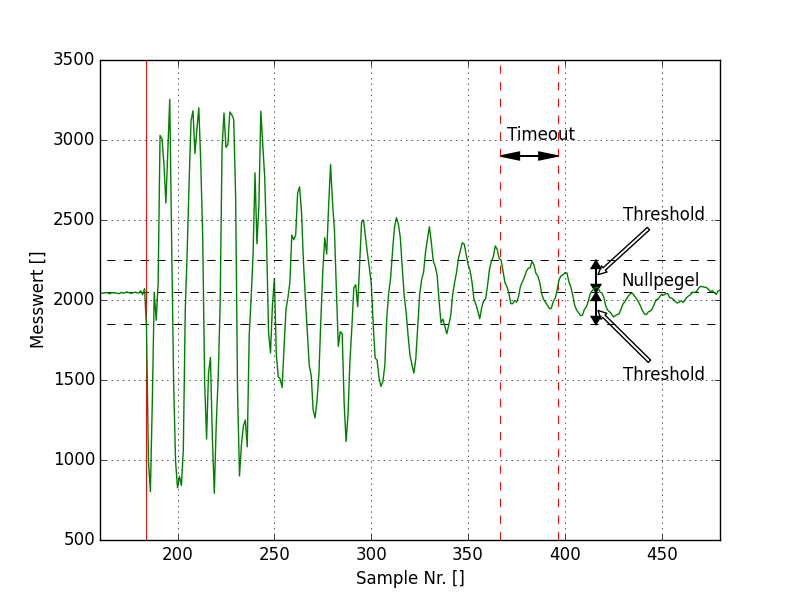
\includegraphics[width=0.8\textwidth]{images/impact_params.png}
	\caption{Zusammenhänge der Parameter der \gls{ereignisdet}.}
	\label{fig.params}
\end{figure}

\begin{lstlisting}[caption=Untermenü Threshold, label=list.paramthres]
 #) Enter threshold value.
    baseline + threshold must not exceed 4096
    and
    baseline - threshold must not be below 0
 0) cancel
\end{lstlisting}

Bei Verletzung der Kriterien für den \gls{threshold} wird eine entsprechende Fehlermeldung angezeigt, Listing \ref{list.paramthresfail}. Da die gleichen Kriterien auch bei der Einstellung des \gls{nullpegel}s gelten, empfiehlt es sich, zuerst einen kleinen Wert für den \gls{threshold} zu wählen. Dann kann der \gls{nullpegel} ohne grosse Einschränkung eingestellt werden. Danach setzt man den passenden \gls{threshold}.

\begin{lstlisting}[caption=Fehlermeldung ungültiger Threshold, label=list.paramthresfail]
 Invalid threshold value:
 threshold + baseline must not exceed 4096
 and
 threshold must be smaller than baseline value.
\end{lstlisting}

\paragraph{Nullpegel} Der \gls{nullpegel} wird mit einer ähnlichen Maske (Listing \ref{list.parambase}) wie der \gls{threshold} eingestellt, auch die Einschränkungen für den Wertebereich sind die Gleichen.

\begin{lstlisting}[caption=Untermenü Null-Level, label=list.parambase]
 #) Enter baseline value (default: 2047).
 0) cancel
\end{lstlisting}

Die Fehlermeldung bei ungültigen Werten für den \gls{nullpegel} ist in Listing \ref{list.parambaseerror} aufgeführt.

\begin{lstlisting}[caption=Fehlermeldung ungültiger Nullpegel, label=list.parambaseerror]
Invalid baseline value:
threshold + baseline must not exceed 4096.
and
threshold - baseline must not be below 0 value
\end{lstlisting}

\paragraph{Timeout} Der \gls{timeout} definiert, wie viele Samples der Signalwert unterhalb des \gls{threshold}s liegen kann, bevor das \gls{ereignis} als beendet betrachtet wird (Listing \ref{list.paramtimeout}). Die Obergrenze für den \gls{timeout} ist 255.

\begin{lstlisting}[caption=Untermenü Timeout, label=list.paramtimeout]
 #) Enter timeout in samples.
 0) cancel
\end{lstlisting}

Bei zu langem (Listing \ref{list.paramtimeoutlong}) oder sehr kurzem (Listing \ref{list.paramtimeoutshort}) \gls{timeout} wird eine Fehlermeldung resp. Warnung angezeigt.

\begin{lstlisting}[caption=Fehlermeldung zu langer Timeout, label=list.paramtimeoutlong]
Timeout too long, can not exceed 512.
\end{lstlisting}

\begin{lstlisting}[caption=Warnung kurzer Timeout, label=list.paramtimeoutshort]
Timeout 0 will end impact after each peak.
Timeout 0 in effect.
\end{lstlisting}

\paragraph{Detaillevel} Über die Wahl des Detaillevels wird bestimmt, wie viele und welche Daten von jedem \gls{ereignis} übertragen und gespeichert werden sollen (Listing \ref{list.detail}). Die Detaillevel sind geordnet nach anfallender Datenmenge, beginnend mit dem grössten Aufwand. Die Detaillevel sind in Abschnitt \ref{sec.manualimpact}, Seite \pageref{sec.manualimpact} beschrieben.

\begin{lstlisting}[caption=Untermenü Detail-Level, label=list.detail]
 1) raw (continuous data)
 2) detailed (start time, all samples of impact)
 3) peaks only (start time, nr of peaks, peaks
 4) sparse (only start time, duration, nr of peaks, max peak)
 5) off
 0) cancel
\end{lstlisting}

\paragraph{Start/Stop Sensor} Jede \gls{sensoreinh} kann einzeln gestartet oder gestoppt werden, vorausgesetzt der \gls{logger} ist gestartet. Im Untermenü ist ersichtlich, in welchem Zustand die ausgewählte \gls{sensoreinh} gerade ist (listing \ref{list.started_one}). Falls die Konfigurationsänderung alle \glspl{sensoreinh} betreffen soll, wird die Anzahl gestarteter und gestoppter Sensoren angezeigt (listing \ref{list.started_all}).

\begin{lstlisting}[caption=Untermenü Start/Stop einzeln, label=list.started_one]
Selected sensor is currently stopped.
 1) start
 2) stop
 0) cancel
\end{lstlisting}

\begin{lstlisting}[caption=Untermenü Start/Stop alle Sensoren, label=list.started_all]
Started sensors: 3
Stopped sensors: 0
 1) start
 2) stop
 0) cancel
\end{lstlisting}

Wenn ein Sensor gestartet wird, muss für die anfallenden Daten eine Datei erzeugt werden. Schlägt dies fehl, wird dies mit der Fehlermeldung \ref{list.sensorerror} angezeigt. Der Sensor wird dann nicht gestartet. Es wird empfohlen, in diesem Fall die SD-Karte zu überprüfen. Möglicherweise verfügt die SD-Karte nicht mehr über genügend Speicherplatz.

\begin{lstlisting}[caption=Fehlermeldung beim Starten eines Sensors, label=list.sensorerror]
Could not create or open file. Please check SD card for free space.
\end{lstlisting}

\subsubsection{Sensor-Status}\label{sssec.sensorstate}
Um die Einstellungen alles Sensoren auf einen Blick zu überprüfen, kann mit dem Befehl 'sensor states' die Liste aller Einstellungen aufgerufen werden, Listing \ref{list.sensorstatus}. In der Liste sind eine interne Nummer, die CAN-Bus-ID, die Seriennummer der \gls{sensoreinh} sowie alle Einstellungen aufgeführt.


\begin{lstlisting}[caption=Untermenü Sensor-Status, label=list.sensorstatus]
Listing sensor config:
 Nr  SID  serial       fs threshold baseline timeout     detail  started?
 1)    2  461bfdf6  10000       200     2047      30        raw      yes
 2)    3  361509a5  10000       150     2000      20 peaks only      yes
 
 0) continue
\end{lstlisting}


\subsubsection{Timestamp zurücksetzen}\label{sssec.timestamp}
Der Timestamp kann manuell zurückgesetzt werden, dafür wird eine Bestätigung eingeholt: Listing \ref{list.timestamp}. Das Zurücksetzen des Timestamps betrifft immer alle \glspl{sensoreinh}.

\begin{lstlisting}[caption=Untermenü Timestamp zurücksetzen, label=list.timestamp]
 1) re-synchronize timestamp
 0) cancel
\end{lstlisting}


\subsubsection{Interne Uhr}\label{sssec.intclock}
Anhand der internen Uhr werden die Timestamps vom \gls{logger} in einen realen Zeitpunkt umgerechnet. Deshalb wird empfohlen, die interne Uhr auf die korrekte Uhrzeit einzustellen. Dies erfolgt über den Befehl 'internal clock', Listing \ref{list.intclock}. Hier kann das Datum (Untermenü \ref{list.setdate}) und die Tageszeit (Untermenü \ref{list.settime}) eingestellt werden.

\begin{lstlisting}[caption=Untermenü interne Uhr, label=list.intclock]
 1) adjust date
 2) adjust time
 0) exit

 current time: Sat Dec 6 18:00:00 2014
\end{lstlisting}

Das Einstellung des Datums erfolgt mit Inkrementen resp. Dekrementen von 365, 30, 10 Tagen oder 1 Tag.

\begin{lstlisting}[caption=Untermenü Datum einstellen, label=list.setdate]
adjust internal date
 1) adjust date +365 days
 2) adjust date -365 days
 3) adjust date + 30 days
 4) adjust date - 30 days
 5) adjust date + 10 days
 6) adjust date - 10 days
 7) adjust date +  1 day
 8) adjust date -  1 day
 0) exit

 current time: Sat Dec 6 18:00:00 2014
\end{lstlisting}

Die Uhrzeit wird mittels Inkrementen resp. Dekrementen von 1 Stunde, 10 oder 1 Minute oder 1 Sekunde eingestellt. Die aktuelle Uhrzeit wird jeweils unterhalb des Menüs angezeigt.

\begin{lstlisting}[caption=Untermenü Uhrzeit einstellen, label=list.settime]
adjust internal time
 1) adjust time +1 hour
 2) adjust time -1 hour
 3) adjust time +10 minute
 4) adjust time -10 minute
 5) adjust time +1 minute
 6) adjust time -1 minute
 7) adjust time +1 second
 8) adjust time -1 second
 0) exit

 current time: Sat Dec 6 18:00:00 2014
\end{lstlisting}

\subsubsection{Konfigurations-Datei}\label{sssec.configfile}

Über den Befehl 'config file' (Listing \ref{list.configfile}) kann die aktuelle Konfiguration der \glspl{sensoreinh} in die Konfigurationsdatei 'config.txt' abgespeichert werden, oder eine neue Konfiguration aus der Datei eingelesen und an die \glspl{sensoreinh} gesendet werden. Es ist nicht möglich, aus mehreren Konfigurationsdateien auszuwählen.

\begin{lstlisting}[caption=Untermenü Konfigurationsdatei, label=list.config]
 1) read configuration from file and set up all sensors accordingly.
 2) store current configuration in file. Old config file will be overwritten.
 0) cancel
\end{lstlisting}

Falls die Konfigurationsdatei nicht gespeichert werden kann, wird die Fehlermeldung in Listing \ref{list.configerror} angezeigt. Um die Konfigurationsdatei trotzdem speichern zu können, kann die SD-Karte abgemeldet und ausgetauscht werden. Die Konfiguration bleibt erhalten, so lange die Spannungsversorgung besteht.

Um einem möglichen Konfigurationsdatenverlust vorzubeugen empfiehlt es sich, die Konfigurationsdatei zu speichern, sobald alle Einstellungen wie gewünscht gemacht wurden. Nach einem Unterbruch in der Spannungsversorgung wird nach automatisch die Konfiguration aus der 

\begin{lstlisting}[caption=Fehlermeldung beim Speichern der Konfigurationsdatei, label=list.configerror]
The config file could not be written. Please check the SD card in a computer.
The configuration data will remain stored in the logger unless you turn off power.
\end{lstlisting}

\subsection{Konfigurationsdatei}
In der Konfigurationsdatei werden die Einstellungen der \glspl{sensoreinh} gespeichert. Die Datei kann auch auf einem \gls{compi} erstellt werden und über eine SD-Karte auf den \gls{logger} übertragen werden. Ein Beispiel einer Konfigurationsdatei zeigt Listing \ref{list.configfile}. Die erste Zeile enthält die Anzahl Datensätze. Jeder Datensatz enthält die Konfiguration einer \gls{sensoreinh}. Auf der zweiten und den folgenden Zeilen folgen die Datensätze. 

Ein Datensatz enthält die CAN-Bus-ID, die Seriennummer der \gls{sensoreinh} als Hexadezimalzahl, die \gls{fs} (ohne die hintersten zwei Nullen), den \gls{threshold}, den \gls{nullpegel} und den \gls{timeout} sowie den Detail-Level und ob der Sensor Daten aufzeichnen soll (1) oder nicht (0).

Der \gls{logger} versucht nach dem Einschalten der Spannungsversorgung die Konfigurationsdatei von der SD-Karte zu lesen. Falls keine SD-Karte vorhanden ist, startet der \gls{logger} den Betrieb nicht, da keine Messdaten gespeichert werden können. Falls die SD-Karte vorhanden ist, aber keine Konfigurationsdatei 'config.txt' enthält, startet der Betrieb der Messstation im Standardmodus.

\paragraph{Standardmodus} Im Standardmodus arbeiten alle \glspl{sensoreinh} mit einer \gls{fs} von \ensuremath{10000 Hz}, \gls{threshold} 200, \gls{nullpegel} 2047, \gls{timeout} 30. Der Detail-Level wird auf 'peaks only' gesetzt, siehe Abschnitt \ref{sec.manualimpact}, Seite \pageref{sec.manualimpact}. Alle \glspl{sensoreinh} werden gestartet.

\begin{lstlisting}[caption=Beispiel einer Konfigurationsdatei, label=list.configfile]
{3,
{2, 461bfdf6, 100, 200, 2047, 30, 3, 1},
{3, 15047b39, 100, 150, 2040, 30, 2, 1},
{4, b78d6dca, 100, 100, 2049, 30, 4, 1},
}
\end{lstlisting}

Falls Änderungen an der Konfiguration gemacht, aber nicht in die Konfigurationsdatei geschrieben wurden, erscheint im Basismenü die Information gemäss Listing \ref{list.configinfo}.

\begin{lstlisting}[caption=Information bei ungespeicherter Konfiguration, label=list.configinfo]
Config has been modified but not saved to SD card.
\end{lstlisting}




\chapter{Verzeichnisse}\label{chap.verzeichnisse}
 %%%%%%%%%%%%%%%%%%%%%%%%%%%%%%%%%%%%%%%%%%%%%%%%%%%%%%%%%%%%%%%%%%
%  _____   ____  _____                                          %
% |_   _| /  __||  __ \    Institute of Computitional Physics   %
%   | |  |  /   | |__) |   Zuercher Hochschule Winterthur       %
%   | |  | (    |  ___/    (University of Applied Sciences)     %
%  _| |_ |  \__ | |        8401 Winterthur, Switzerland         %
% |_____| \____||_|                                             %
%%%%%%%%%%%%%%%%%%%%%%%%%%%%%%%%%%%%%%%%%%%%%%%%%%%%%%%%%%%%%%%%%
%
% Project     : LaTeX doc Vorlage für Windows ProTeXt mit TexMakerX
% Title       : 
% File        : literatur.tex Rev. 00
% Date        : 23.4.12
% Author      : Remo Ritzmann
% Feedback bitte an Email: remo.ritzmann@pfunzle.ch
%
%%%%%%%%%%%%%%%%%%%%%%%%%%%%%%%%%%%%%%%%%%%%%%%%%%%%%%%%%%%%%%%%%

\begin{thebibliography}{99}
\addcontentsline{toc}{section}{Literaturverzeichnis}\label{cha:literaturverzeichnis}

% How to make a Literaturlist nach www.ieee.org/documents/ieeecitationref.pdf
% Erklärung

%Books
\bibitem{robotvision} B. Klaus and P. Horn, Robot Vision. Cambridge, MA: MIT Press, 1986.
%Einzelne Seiten aus Buch
\bibitem{randompatterns} L. Stein, ">Random patterns,"> in Computers and You, J. S. Brake, Ed. New York: Wiley, 1994, pp. 55-70.



\end{thebibliography}

\Urlmuskip=0mu plus 1mu\relax
 %\bibliographystyle{plain}
 \bibliographystyle{bibtex}
 \begingroup
 \raggedright
 \bibliography{literatur}
 \endgroup \newpage
 \listoffigures
 %\addcontentsline{toc}{section}{(Abbildungsverzeichnis)}
 \listoftables
 %\addcontentsline{toc}{section}{(Tabellenverzeichnis)}
 \deftranslation[to=German]{Acronyms}{Abk�rzungsverzeichnis}
 \deftranslation[to=German]{Glossary}{Glossar}
 \printglossary
 %\addcontentsline{toc}{section}{(Glossar)}
 \printglossary[type=acronym]
 % \addcontentsline{toc}{section}{(Abk�rzungen)}
 \lstlistoflistings
 %\addcontentsline{toc}{section}{(Listingverzeichnis)}
 
% !TeX spellcheck = de_CH
%%%%%%%%%%%%%%%%%%%%%%%%%%%%%%%%%%%%%%%%%%%%%%%%%%%%%%%%%%%%%%%%%
%  _____   ____  _____                                          %
% |_   _| /  __||  __ \    Institute of Computitional Physics   %
%   | |  |  /   | |__) |   Zuercher Hochschule Winterthur       %
%   | |  | (    |  ___/    (University of Applied Sciences)     %
%  _| |_ |  \__ | |        8401 Winterthur, Switzerland         %
% |_____| \____||_|                                             %
%%%%%%%%%%%%%%%%%%%%%%%%%%%%%%%%%%%%%%%%%%%%%%%%%%%%%%%%%%%%%%%%%
%
% Project     : BA Welti Keller
% Title       : 
% File        : anhang.tex Rev. 00
% Date        : 15.09.2014
% Author      : Tobias Welti
%
%%%%%%%%%%%%%%%%%%%%%%%%%%%%%%%%%%%%%%%%%%%%%%%%%%%%%%%%%%%%%%%%%


\pagenumbering{Roman}

\appendix
\chapter{Anhang}\label{chap.anhang}



\section{Projektmanagement}\label{sec.projektmanagement}

\begin{itemize}
\item Offizielle Aufgabenstellung, Projektauftrag
\item (Zeitplan)
\item (Besprechungsprotokolle oder Journals)
\end{itemize}



\section{Weiteres}\label{weiteres}

\begin{itemize}
\item CD mit dem vollständigen Bericht als pdf-File inklusive Film- und Fotomaterial
\item (Schaltpläne und Ablaufschemata)
\item (Spezifikationen u. Datenblätter der verwendeten Messgeräte und/oder Komponenten)
\item (Berechnungen, Messwerte, Simulationsresultate)
\item (Stoffdaten)
\item (Fehlerrechnungen mit Messunsicherheiten)
\item (Grafische Darstellungen, Fotos)
\item (Datenträger mit weiteren Daten (z.B. Software-Komponenten) inkl. Verzeichnis der auf diesem Datenträger abgelegten Dateien)
\item (Softwarecode)
\end{itemize}



\end{document}
